%%%
% Ami lecteur, bonjour !
%
% Ce fichier regroupe les commandes utilis�es par les �ditions H&K pour
% l'�laboration des Annales des Concours. Si vous �tes auteur dans cette
% collection, vous trouverez de nombreuses explications dans la documentation
% disponible sur http://auteurs.h-k.fr�.
%
% Les auteurs des Annales des Concours sont explicitement autoris�s �
% r�utiliser tout ou partie de ce fichier pour leurs travaux personnels 
% � but non commercial (m�moire, rapport, th�se, cours, colles, etc.).
% 
% Si vous n'avez pas particip� aux Annales des Concours, veuillez contacter
% directement les �ditions H&K (contact@h-k.fr) si vous souhaitez utiliser
% ce fichier.
%
% Les macros propos�es ci-dessous ont n�cessit� des centaines d'heures de
% travail. Elles ne sont pas dans le domaine public, hormis l'environnement
% \breakbox.
%
%                                                         Seb.
%
%
% Le mainteneur du fichier peut toujours �tre joint � l'adresse
% annales.sty@H-K.fr
%
% 2001.11.03:	* Migration de certains \mathop vers \DeclareMathOperator.
%               * Ajout des symboles chimiques � deux lettres (\Al, etc.).
%               * Ajout de [t] et d'une option dans {rcl}.
% 2001.11.27:	* Correction d'un bug dans \leftcentersright.
% 2001.12.06:	* Ajout de \Me, \liq, \sol, \gaz et \Equilibre.
% 2001.12.07: 	* Ajout de l'option [t] dans \leqsystsimple.
%               * Ajout de \Image.
% 2001.12.08:	* Changement de police pour \apriori et ses amis.
% 2001.12.11:	* Ajout de \abs pour les valeurs absolues.
% 2002.02.21:	* Ajout de \Dpc et \DPC (Teteph)
% 2002.04.19:	* Ajout de \note
% 2002.04.20:	* Passage de fancyheadings � fancyhdr (suggestion de JJ).
% 2002.04.21:	* Cr�ation \(leftcenters|centers|ref)numero (JJ).
% 2002.04.22:	* Ajout de \accolades et \paa (David Chapot, JJ).
% 2002.05.12:	* Retrait d'un espace dans \cf.
%               * Retrait des \left et \right dans \intn (Walter).
% 2002.05.16:	* Correction de \RX et \CX (Jean).
% 2002.05.17:	* Ajout du package {tabularx} (JJ).
% 2002.05.24:	* Retrait de {tabularx}.
% 2002.05.31:	* Correction de \ANcenters et \ANencadre (JJ).
% 2002.06.14:	* Modification de \enonce pour faire des hachures.
% 2002.06.19:	* Modification de \celsius (BBR).
%               * Cr�ation de la commande \angstrom (BBR, Teteph).
% 2002.06.24:	* Modification de \Star (Alex).
% 2002.06.25:	* Cr�ation de \conc et \Kzero (Alex).
% 2002.06.26:	* Cr�ation de \serie (Walter).
% 2002.06.27:	* Cr�ation de \butyl et \Bu (Alex).
% 2002.06.28:	* Modification de \ANcenters et \ANencadre (Alex).
% 2002.06.30:	* Modification de \degres (BBR).
% 2002.07.04:	* Modification de \celsius (Nico).
% 2002.07.08:	* Modification de \etc (JJ).
% 2002.07.08:	* Modification de \cf: droit, point (�milia).
% 2002.07.12:	* Ajout de \intnn (Mathieu).
% 2002.07.16:	* Abandon de fancyhdr pour fancyheadings � cause des titres
%                 courants dans les annexes (JJ).
% 2002.08.14:	* D�coupage du fichier en trois morceaux ind�pendants:
%                 d�clarations, mise en page et commandes scientifiques.
%               * R��criture de la plupart des commentaires contextuels.
% 2003.02.12:	* Cas des arguments vides dans \intff et al (Walter).
% 2003.03.05:	* Modification de la commande \partie (Paul).
% 2003.03.10:	* Remplacement des \mathbb par des \mathBB (Paul).
% 2003.03.18:   * Ajout de la commande \reperes (VF).
% 2003.05.05:	* Passage � des titres courants centr�s (Paul).
% 2003.05.11:	* Ajout de \mathaccent"17E (JJ).
% 2003.05.21:	* Ajout de \ir, \jr, \ex et \exi (Paul et VF).
% 2003.05.26:	* Ajout de \OIInt (TTF, ST) et de \sulfate (Manu).
% 2003.05.27:	* Ajout de \vectux, \vectuy, \vectuz, \vectex, \vectey,
%                 \vectez, \vux, \vuy, \vuz, \vex, \vey et \vez.
% 2003.06.01:	* Ajout de \suite et \liste (Paul).
% 2003.06.06:	* Ajout de dsfont.sty pour \mathds{1}.
% 2003.06.28:	* Cr�ation de \petito et \grando (JJ, Walter, Paul).
% 2003.06.29:	* Ajout de \pmgras (Mike).
% 2003.06.30:	* Cr�ation de \Sumt (Walter).
% 2003.10.16:	* Ajout de \NoAutoSpaceBeforeFDP dans \codesource (Walter).
% 2003.10.23:	* Ajout de \NoAutoSpaceBeforeFDP dans \web.
% 2003.12.07:	* Ajout de \encadreminipage (Aur�lien).
% 2003.12.08:	* Ajout de \graphicspath
% 2004.02.19:	* Ajout de \Produit (Paul, C�line).
% 2004.02.21:	* Ajout de \scalar (C�line).
% 2004.02.27:	* Am�lioration de \intff et ses amis (C�line).
% 2004.03.06:	* Red�finition de \bs (Seb, C�line).
% 2004.03.08:	* Am�lioration de \leftcentersright et ses d�riv�s: l'argument
%                 du milieu est maintenant centr� dans la page, pas dans
%                 l'environnement (C�line, Paul).
% 2004.03.09:	* Bug-fix dans \Sum (port�e de \ensuremath) (C�line).
% 2004.03.15:   * Ajout de \ofg pour les guillemets fran�ais (Manu).
% 2004.03.16:   * Passage de fancyheadings � fancyhdr.
% 2004.03.18:   * Ajout des environnements {egalites}, {inegalites:leq}, 
%                 {inegalites:geq}, {calculs}, {calculs:rcl}, 
%                 {calculs:rcl:extracol} et {calculs:latotale}
%                 (C�line, Paul, Seb, JB)
% 2004.03.20:   * Modification de la commande \note; par d�faut, elle
%                 rajoute un num�ro � l'endroit o� on l'appelle et avec
%                 l'option 0 ou simple elle reprend son ancien
%                 comportement (JJ)
%               * Am�lioration de \Sum, \SUM et \Int (JJ)
%               * Modification des commandes \partie, \Partie et
%                 \Indications pour pouvoir obtenir les petites
%                 capitales m�me avec aeguill (JJ)
% 2004.03.22:   * Changement de l'option d'alignement par d�faut dans
%                 les environnements {systsimple} et d�riv�s
%               * \finalementcenters donne d�sormais � Finalement, � au 
%                 lieu de � Finalement: � .
%               * Modification des tailles du papier et des marges (Seb).
% 2004.03.25:	* Modification de la l�gende des sommaires crois�s.
% 2004.03.29:	* Ajout de \Rdeux, \Rtrois, \Cdeux et \Ctrois.
% 2004.04.01:	* Ajout de \centersminipage (Seb).
% 2004.04.03:   * Transfert des commandes pour les sommaires crois�s
%                 vers les fichiers concern�s.
% 2004.04.04:	* Retrait de {aeguill}.
% 2004.04.08:   * Bug-fix dans un commentaire (Seb).
% 2004.04.09:   * Suppression du commentaire sur l'installation TeX
%                 d'Ulm (FX).
% 2004.04.18:	* Ajout de \notemark et \notetext pour pouvoir utiliser
%                 \note dans n'importe quel environnement.
%               * Ajout de \arraybox pour remplacer \EncadreDansTableau.
% 2004.04.20:   * Ajout de \typeout dans \EncadreDansTableau (Teteph).
% 2004.04.23:	* Abandon de la police Times dans \partie.
%               * Ajout de l'option dans \donccenters et ses amis.
% 2004.04.30:	* Ajout de \DecimalMathComma (Paul).
% 2004.05.04:	* Passage � \StandardMathComma par d�faut (Teteph).
% 2004.05.05:	* Correction d'un bug dans \leftcentersright.
% 2004.05.08:	* Ajout de \aq (FX).
% 2004.05.14:	* Ajout de \null dans les \qetq.
%               * Modification de \leftcentersright: l'argument est
%                 toujours centr� dans la page, sauf dans les
%                 {remarque} (Manu).
%               * Ajout de \textegras, \textgras, \gras, \nongras,
%                 modification de \mathBB, \mathscr, 
%                 \partie et \Partie (Walter).
% 2004.05.15:   * Ajout de \thallium et \Tl (Alex).
%               * Ajout de \Pzero et \czero (FX).
%               * Ajout de \base.
% 2004.05.16:   * Ajout de \Rb et \rubidium (Tiphaine).
% 2004.05.17:	* \mathscr renomm� en \mathscrchoice (Seb).
% 2004.05.18:	* Ajout de \Iint et \IInt. Modification des longueurs
%                 dans \oiint et \OIInt (Marc, Paul).
% 2004.05.19:	* Ajout de \deltar et \deltaf (Alex).
% 2004.05.20:	* Ajout de \Avogadro et \avogadro (JJ).
% 2004.05.21:	* Retrait de \Avogadro et \avogadro pour ne pas
%                 privil�gier de notation.
% 2004.05.22:	* Ajout de \exmi (Aur�lien).
%               * Ajout de \Ce et \cerium (Alex).
% 2004.05.26:	* Red�finition de \venonce (Alex).
% 2004.05.27:	* Ajout de \uvect (Aur�lien).
%               * Ajout de \encadrenumero et \leftencadrenumero (Aur�lien).
% 2004.05.28:	* Ajout de \vectu (Aur�lien).
% 2004.05.31:	* Ajout de \Zr et \zirconium (Nicolas).
% 2004.06.09:	* Am�lioration de \simple, \double, \triple (FX).
% 2004.06.11:   * Am�lioration de \pm et \pmgras (Vincent).
% 2004.06.14:   * Retrait de \typeout dans \EncadreDansTableau.
% 2004.06.17:   * Ajout de \indenter (Teteph).
%               * Modification de \centers pour proteger l'argument central
%                 (Teteph).
% 2004.07.01:   * Ajout d'une option � \titre (Teteph).
% 2004.07.02:   * Modification de \petito et \grando (David, Seb).
% 2004.07.03:   * Ajout de \ajusterletitrecourant.
% 2004.07.05:   * Remplacement de \LeTitre par \LeTitreCourant dans les
%                 commandes \titresommaire, \JusteNumeroPage, \mkTitreCourant.
% 2004.11.02:   * Am�lioration de \pm et \pmgras (Emmanuel).
%               * Changement du \renewcommand en \def dans la d�finition de
%                 \degres car la commande \degres n'existe plus sur clipper
%                 � l'ENS.
% 2004.12.09:   * Ajout de \xspace dans les d�finitions des raccourcis
%                 \droite, \plan, \cercle, etc (Seb).
%               * Ajout d'une bascule (\CentersOnPage (d�faut) et 
%                 \CentersOnItems) pour que \centers centre soit par rapport �
%                 la page soit par rapport � l'{itemize}. Cette bascule est
%                 remise � sa valeur par d�faut dans la commande \titre (Seb). 
% 2004.12.17:   * Ajout de \arcdecercle (JJ).
% 2005.01.02:   * Ajout de \email (Seb).
% 2005.05.06:   * Ajout de \partieentieresup (Sam).
% 2005.05.07:   * Ajout de \oeuf et \oeufs (Seb).
% 2005.05.24:   * Ajout de \maitre (Seb).
%               * Am�lioration de \madame, \mademoiselle, \docteur, \maitre.
% 2005.05.30:   * Ajout de \Iiint et \IIInt (Teteph).
% 2005.06.05:   * Ajout de \matricedd.
% 2005.06.07:   * Ajout des \xspace dans \R, \C et commandes similaires.
% 2005.06.28:   * Am�lioration de \pa (Vincent).
% 2005.06.29:   * Am�lioration de \pac et \paa (Teteph).
% 2005.07.08:   * Ajout de \Sm, \samarium, \Eu, \europium (Alex).
% 2005.07.12:   * Ajout de \tdemi, \ttiers, \tquart (Alex).
%               * Mise � jour de la l�gende des sommaires crois�s.
% 2005.07.15:   * Modification des commandes � base de \mathBB: l'ajout de
%                 \xspace faisait buguer la version �toil�e (David).
%				* Ajout du package longtable et modification du sommaire
%                 (JJ).
% 2006.03.28:   * Modification des marges due au changement de format (pas de 
%                 changement de la taille du texte) (JJ).
% 2006.05.12:   * Ajout de \dessinpgf pour les courbes cr��es avec les 
%                 extensions LaTeX PGF et TikZ (Teteph).
% 2006.05.14:   * Ajout de \indicatrice.
%               * Changement de la d�finition de \ronde et \angstrom (Seb, 
%                 JJ).
% 2006.05.16:   * Ajout de \soeur, \soeurs, \Soeur, \Soeurs (Sattisvar).
% 2006.05.23:   * Ajout de \vcol (Aur�lien, Fr�d�ric).
%               * Am�lioration de \moyenne (Teteph).
% 2006.05.25:   * Ajout de \souspartie (Teteph, Seb).
% 2006.05.31:   * Ajout de \transp (Aur�lien, Seb).
% 2006.06.02:   * Ajout de \fem et \AO (Aur�lien, Seb).
%               * Modification de \transp (qui devient synonyme de \trans).
% 2006.06.06:   * Modification de \f@thousandsep, utilis�e dans \nombre.
%               * Ajout de \nb, raccourci pour \nombre.
% 2006.06.12:   * Modification des tailles des marges (Alex).
% 2006.06.14:   * Bug-fix de l'alignement de {QCM} (Aur�lien).
% 2006.06.18:   * Ajout du test sur les . et - dans \souspartie.
% 2006.06.27:   * Ajout d'un argument optionnel � \norme (Teteph).
% 2006.07.07:   * Modification de \partie et \Partie.
% 2006.07.08:   * Annulation de la modification de \partie et \Partie 
%                 (Teteph).
% 2006.07.08:   * Am�lioration de \dessinpgf (Teteph).
% 2006.07.09:   * Ajout de \kdonne (Alex).
% 2006.07.11:   * Modification des commandes pour les sommaires: ajout de 
%                 \tdmtabular, \tdmoutils, \tdmtitresommaire et \tdmConcours.
% 2006.07.11:   * Modification de la l�gende des sommaires crois�s.
% 2007.05.02:   * Ajout de \ver, \verho, \vetheta, \vephi, \vur, \vurho, 
%                 \vutheta et \vuphi (Emmanuel Loyer).
% 2007.05.21:   * Ajout des commandes pour dessiner les rectangles gris: 
%                 \dessinerRectangleGris, \rectangleGrisOUI, 
%                 \rectangleGrisNON (Seb).
%               * Modification de la taille du papier (17,5 par 26) pour 
%                 tenir compte des fonds perdus dus � ces rectangles.
%               * Ajout des commandes pour les formulaires: \vartitre, 
%                 \formulairesMaths, \formulairePhysiqueChimie.
%				* Modification de \tdmtabular pour le sommaire.
% 2007.05.23:   * Ajout de \Sc et \scandium (Nicolas Agenet).
% 2007.06.17:   * Ajout de \versionCompil qui g�re les marges et les notes.
% 2007.06.27:   * Modification de la taille du papier pour centrer le texte 
%                 sur la page (Teteph, Seb).
%               * Ajout de \relpenalty et \binoppenalty pour �viter la coupure 
%                 des formules de maths (Teteph).
% 2007.07.01:   * Ajout d'un argument optionnel � \souspartie (Teteph).
% 2007.07.07:   * Suppression des commandes obsol�tes pour les marges 
%                 (Teteph).
%               * Ajout de \textgras dans \souspartie (Jean).
% 2007.07.11:   * Ajout de \raggedright dans \tdmoutils (Teteph et Seb).
%               * Mise � jour de la l�gende des sommaires crois�s.
%               * Suppression de \relpenalty et \binoppenalty (JJ).
%               * Modification de \tdmENAC.
% 2007.11.13:   * Ajout d'\euros comme synonyme d'\euro (Seb).
% 2008.03.29:   * Modification de \versionCompil, \enonce et \venonce pour les
%                 bandes grises (Seb).
% 2008.04.09:   * Bug-fix dans \ajusterletitrecourant (Seb).
% 2008.04.24:   * R�tablissement de \relpenalty et \binoppenalty (Teteph).
%               * Ajout d'un bool�en weAreInUnitsMode dans \U, utilisation
%                 dans \celsius et ajout de la commande \kelvin (Seb).
% 2008.05.01:   * D�placement de \relpenalty et \binoppenalty hors de 
%                 \versionCompil (Teteph).
% 2008.05.19:   * Ajout de \plutonium et \Pu (Tiphaine).
% 2008.05.24:   * Ajout de \oldRe et \oldIm (David).
% 2008.06.28:   * Modification de \versionCompil, \enonce et \venonce pour      
%                 les bandes grises (Seb).
% 2008.07.05:   * Ajout de \overfullrule r�gl� � 1 cm (Seb).
%               * Retour � l'ancienne version de \celsius (JJ, Teteph).
% 2008.07.06:   * Suppression de l'\overfullrule qui pose probl�me dans les 
%                 dessins et cr�ation de \versionAuteur (JJ, Seb).
% 2008.07.07:   * Ajout de \zk pour annuler les \mk et ses amis (Seb).
% 2008.07.08:   * Ajout de \qSSIq et \qqSSIqq (Jean et JJ).
% 2008.07.09:   * Ajout de \faraday et \Faraday (Seb).
% 2008.07.10:	* Modification de la l�gende des sommaires crois�s.
%               * Ajout de \bandeGrise (Seb).
% 2008.10.16:   * Ajout de \proportionnel (Seb).
% 2009.04.27:   * Modification de \ddf, \ddt, \ddxx, \ddtt, \Dp, \Dpt, \DDp, 
%                 \DP pour leur ajouter un argument optionnel (Teteph, Mike).
% 2009.05.01:   * Ajout de \Au (Mike). 
% 2009.05.14:   * Ajout de \mathpzc dans les polices exotiques (C�line).
% 2009.06.07:   * Ajout d'une option � \arraybox (JJ, C�line).
% 2009.07.07:   * Mise � jour de la l�gende des sommaires crois�s.
% 2009.07.09:   * Ajout d'un \raggedright dans la colonne R�sum�s de 
%                 {tdmtabular}.
% 2009.07.10:   * Ajout de \pubpage pour inclure des pages de pub.
% 2009.10.17:   * Ajout de \pictoRemarque, \pictoRq et \pictoRapport pour 
%                 inclure les pictos.
% 2009.10.18:   * Ajout du package eurosym.
% 2010.02.12:   * Modification de la commande \pictoRemarqueImage pour inclure
%                 la boussole en version Compil.
% 2010.07.09:   * Mise � jour de la l�gende des sommaires crois�s.
% 2010.07.12:   * Modification de \titre et \ajusterletitrecourant afin de 
%                 permettre la s�lection des premi�res pages (Seb).
% 2010.10.15:   * Modification de \codesource pour introduire la commande
%                 \errmessage afin d'interrompre la compilation si le fichier
%                 est introuvable (Seb, C�line).
% 2010.11.04:   * Ajout de \epsfigpicture pour placer un dessin ��� la main��
%                 (JJ).
%               * Ajout de \underbracket, �quivalent de \underbrace (C�line).
%               * Red�finition de \@onefilewithoptions pour que la compilation
%                 continue en cas de package manquant (C�line).
% 2011.01.05:	* Extension de \graphicspath et �limination du chemin vers
%				  billeBoussole.ps dans \pictoRemarque (Seb).
% 2011.06.12:   * Ajout de \nieme (C�line).
%               * Modification de \pinf et \minf (C�line).
% 2011.07.03:   * Mise � jour de la l�gende des sommaires crois�s et cr�ation 
%				  de \tdmEAAA.
% 2012.06.11:   * Modification de \Cte (Tom Morel, C�line).
% 2012.07.02:   * Mise � jour de la l�gende des sommaires crois�s.
% 2013.05.05:	* Red�finition de \hk et \vk.
% 2014.04.10:	* Ajout des commandes pour les probas (Walter).
% 2014.06.24:	* Ajout de \dxyz et \ddxyz (Jimmy).
% 2015.03.01:	* Modification de \ANcenters et \ANencadre (Alex, VT)
%				* Am�lioration de \Sum (Sadik)
%				* Am�lioration de \matricedd (Sadik)
%				* \page et \Page n'apparaissent plus en bas de page (Sadik)
%				* Ajout de \vpush (Sadik)
%				* Modification de \sk, \mk, \bk, \leftcentersright, \question,
%				  {remarque}, {calculs:base}, {calculs:rcl:extracol}, 
%				  {calculs:rcl} et {calculs:latotale} pour utiliser \vpush
%				* Cr�ation de \sk*, \mk* et \bk*
%				* Diminution des espaces avant/apr�s {remarque}: \bk -> \mk
%				* Simplification des noms pour les d�riv�es (\der, etc.).
% 2015-05-01:	* Ajout de \derpx, \derpy, \derpz, \derPx, \derPy, \derPz 
%				  (�tienne Th.).
% 2015-07-07:	* Ajout de \questionremarque.
% 2015-07-14:	* Ajout de \qouq et \qqouqq.
% 2017-07-25:	* Red�finition de \addpenalty.
% 2018-06-20:	* Ajout d'\epsfigright et \epsfigleft (Teteph).
% 2018.07.03:	* Cr�ation de \rhodium et \Rh (Alex).
% Delete presentation newcommand
% Delete note newcommand
% Delete paper size settings
% Delete page structure
% Delete commandes de titre
% Delete vmargin and papersize commands
%%%

% Le code suivant permet d'�viter que la compilation d'un document �choue
% lorsqu'un package appel� dans ce fichier est absent de l'ordinateur. Ceci
% permet aux auteurs qui ont une installation raisonnablement r�cente de
% LaTeX d'utiliser les possibilit�s de cette derni�re tout en garantissant la
% compatibilit� avec les installations plus anciennes chez d'autres auteurs.
% Ceux-ci sont tout de m�me p�nalis�s dans la mesure o� les commandes
% contenues dans les packages appel�s ne fonctionnent pas, pas plus que les
% commandes de ce fichier qui s'appuient sur elle; mais au moins, le
% document compile.
% Ce code doit imp�rativement �tre situ� avant \documentclass.

\makeatletter
\def\@onefilewithoptions#1[#2][#3]#4{%
  \@pushfilename
  \xdef\@currname{#1}%
  \global\let\@currext#4%
  \expandafter\let\csname\@currname.\@currext-h@@k\endcsname\@empty
  \let\CurrentOption\@empty
  \@reset@ptions
  \makeatletter
  \def\reserved@a{%
    \@ifl@aded\@currext{#1}%
      {\@if@ptions\@currext{#1}{#2}{}%
        {\@latex@error
            {Option clash for \@cls@pkg\space #1}%
            {The package #1 has already been loaded
             with options:\MessageBreak
             \space\space[\@ptionlist{#1.\@currext}]\MessageBreak
             There has now been an attempt to load it
              with options\MessageBreak
             \space\space[#2]\MessageBreak
             Adding the global options:\MessageBreak
             \space\space
                  \@ptionlist{#1.\@currext},#2\MessageBreak
             to your \noexpand\documentclass declaration may fix this.%
             \MessageBreak
             Try typing \space <return> \space to proceed.}}}%
      {\@pass@ptions\@currext{#2}{#1}%
       \global\expandafter
       \let\csname ver@\@currname.\@currext\endcsname\@empty
       \InputIfFileExists
         {\@currname.\@currext}%
         {}%
         {%
        \typeout{^^J^^J%
                Le package "#1.sty" n'est pas disponible sur cet ordinateur�!
        }%
        \typeout{%
                Les commandes qui l'utilisent ne fonctionneront pas.
        ^^J^^J}%
         }%
%         {\@missingfileerror\@currname\@currext}%
    \let\@unprocessedoptions\@@unprocessedoptions
    \csname\@currname.\@currext-h@@k\endcsname
    \expandafter\let\csname\@currname.\@currext-h@@k\endcsname
              \@undefined
    \@unprocessedoptions}
    \@ifl@ter\@currext{#1}{#3}{}%
      {\@latex@warning@no@line
         {You have requested,\on@line,
          version\MessageBreak
            `#3' of \@cls@pkg\space #1,\MessageBreak
          but only version\MessageBreak
           `\csname ver@#1.\@currext\endcsname'\MessageBreak
          is available}}%
    \ifx\@currext\@clsextension\let\LoadClass\@twoloadclasserror\fi
    \@popfilename
    \@reset@ptions}%
  \reserved@a}
\makeatother


\documentclass{beamer}

%!!!!!!!!!!!!!!!!!!!!!!!!!!                  !!!!!!!!!!!!!!!!!!!!!!!!!!
%!!!!!!!!!!!!!!!!!!!!!!!!!!   Les packages   !!!!!!!!!!!!!!!!!!!!!!!!!!
%!!!!!!!!!!!!!!!!!!!!!!!!!!                  !!!!!!!!!!!!!!!!!!!!!!!!!!

%% Les packages � charger en standard.

\usepackage[frenchb]{babel}	% Typo francaise.
\FrenchItemizeSpacingfalse	% Pour avoir des \bullet dans les {itemize}
            				% et ne pas d�r�gler les espaces verticaux.
\usepackage[T1]{fontenc}	% Accents cod�s dans la fonte.
\usepackage[latin1]{inputenc}	% Accents 8 bits dans le fichier.
%\usepackage{vmargin}		% R�gler la taille de la feuille.
\usepackage{fancyhdr}		% R�gler le titre courant et le bas de page.
%\usepackage{fancyheadings}
\usepackage{calc}	    	% Faire des calculs sur les longueurs.
\usepackage{ifthen}		    % Faire des tests if/then/else.
\usepackage{pifont}		    % La police \ding.
\usepackage{eurosym}		% Le symbole \euro.
\usepackage{supertabular}	% Les grands tableaux.
\usepackage{longtable}
\usepackage{multicol}		% Plusieurs colonnes.
\usepackage{wrapfig}		% Dessins dans le texte.
\usepackage{fancybox}		% Bo�tes avec une ombre pour les parties.
\usepackage{rotating}		% Pour tourner un texte.
\usepackage{xspace}		    % Ajuster l'espace apr�s des mots.

%% Les packages pour les maths.

\usepackage{amsmath}	% Les symboles les plus fr�quents.
\usepackage{amssymb}	% Des symboles.
\usepackage{amsfonts}	% Des fontes, eg pour \mathbb.
\usepackage{verbatim}	% Pour les codes sources en informatique.
\usepackage{mathrsfs}	% Des lettres majuscules cursives (\mathscr).
\usepackage{dsfont}

%% Les packages pour les dessins.

\usepackage{array}
\usepackage{curves}
\usepackage{epic}
\usepackage{eepic}
\usepackage{epsfig}
\usepackage{graphics}
\graphicspath{{PS/}{../../config/PS/}{PS_peripheries/}}

%!!!!!!!!!!!!!!!!!!!!!!!!!!!!              !!!!!!!!!!!!!!!!!!!!!!!!!!!!
%!!!!!!!!!!!!!!!!!!!!!!!!!!!!   Bugfixes   !!!!!!!!!!!!!!!!!!!!!!!!!!!!
%!!!!!!!!!!!!!!!!!!!!!!!!!!!!              !!!!!!!!!!!!!!!!!!!!!!!!!!!!

% Jusqu'en 2014, le moteur de LaTeX incluait un bug l�ger dans \addpenalty, du 
% fichier ltspace.dtx (dans une TeXLive). Il �tait corrig� via le fichier 
% fixltx2e.dtx, qui �tait appel� en \usepackage. ��partir de 2015, TeXLive a 
% fusionn� ces fichiers. Or le changement dans la d�finition de \addpenalty a 
% fait que des corrig�s compilaient diff�remment selon qu'ils �taient compil�s 
% sur une TeXLive 2014 (qui �tait incluse dans la Debian stable d�but 2017) ou 
% sur une TeXLive 2015+ (cas d'Ubuntu et de la nouvelle Debian stable arriv�e 
% en milieu de session). La correction de ce bug n'am�liore pas les Annales en 
% pratique. Il est plus important que la compilation soit la m�me partout.
% C'est pourquoi on met ci-dessous l'ancienne d�finition de \addpenalty.

\makeatletter
\def\addpenalty#1{%
  \ifvmode
    \if@minipage
    \else
      \if@nobreak
      \else
        \ifdim\lastskip=\z@
          \penalty#1\relax
        \else
          \@tempskipb\lastskip
          \vskip -\lastskip
          \penalty#1%
          \vskip\@tempskipb
        \fi
      \fi
    \fi
  \else
    \@noitemerr
  \fi}
\makeatother


%!!!!!!!!!!!!!!!!!!!!!!                          !!!!!!!!!!!!!!!!!!!!!!
%!!!!!!!!!!!!!!!!!!!!!!   Pr�sentation globale   !!!!!!!!!!!!!!!!!!!!!!
%!!!!!!!!!!!!!!!!!!!!!!                          !!!!!!!!!!!!!!!!!!!!!!

%% La commande centralisant les r�glages sp�cifiques aux versions de travail.

\newcommand{\versionAuteur}{
	% Montrer les overfull � l'aide de carr�s noirs.
	\setlength{\overfullrule}{1cm}
}

%% La commande centralisant les changements n�cessaires � la compil.
%% L'argument est le nombre de corrig�s; il sert � ajuster la taille des
%% rectangles dans les �nonc�s.

\newboolean{versionPostCompilPourArchivage}                                   
% � ajouter *en plus* de \versionCompil, *avant* \versionCompil.
\newcommand\versionPostCompilPourArchivage{%                                  
      \setboolean{versionPostCompilPourArchivage}{true}                       
} 

\newboolean{versionCompil}
\newcounter{nombreDeCorriges}
\newcommand{\versionCompil}[1][1]{%

	\setboolean{versionCompil}{true}                                        
	\setcounter{nombreDeCorriges}{#1}% On en fait une variable globale    
		% pour pouvoir l'utiliser dans \enonce. 

    % Octobre 2012: la hauteur du livre passe � 24�cm (pb approvisionnement 
	% papier)
	%\setpapersize{custom}{17.5cm}{25.0cm}%
	%\setmarginsrb{22.5mm}{5.5mm}{23.5mm}{9.5mm}{10mm}{6mm}{0mm}{5mm}%

    % Jusqu'en octobre 2012 et de nouveau � partir de juin 2013:

		% Attention, lors de l'export en postscript, il faut alors passer       
		% l'option -T17.5cm,26cm � dvips.                                       
		% En TeTeX 3, il faut �galement l'option -tunknown pour dvips.   
                                                                        
	\AtEndDocument{%                                                       
		\typeout{}%                                                     
		\ifthenelse{\boolean{versionPostCompilPourArchivage}}{%         
			\typeout{dvips main.dvi -tunknown -R0 -T17cm,25cm -o}% 
		}{%                                                             
			\typeout{dvips main.dvi -tunknown -R0 -T17.5cm,26cm -o}%
		}                                                               
		\typeout{}%                                                     
	}                             

    % Ne plus montrer les notes.
    \setcounter{ifnote}{0}%

	% Charger la police EuScript pour le corrig� MP_MATHS_CENTRALE_2_2008.
	\policesExotiquesAvecAutorisationDuCoordinateur{1}%
	\policesExotiquesAvecAutorisationDuCoordinateur{2}%

	%%                                                                      
	%% On ajoute maintenant les bandes grises.                              
	%%                                                                      

	\usepackage[absolute]{textpos}                                          

	% Le r�glage suivant permet de consid�rer que le coin en haut �         
	% gauche de la page (dans les dimensions \versionCompil) comme ayant 
	% les coordonn�es (0pt,0pt). On donne ensuite les positions dans 
	% {textblock*}: d'abord le d�calage vers la droite, ensuite le d�calage 
	% vers le bas.          
	\textblockorigin{57.35pt}{72.35pt}                                      
                                                                            
	\usepackage{color} 
	\definecolor{grayband}{cmyk}{0, 0, 0, 0.5}                              

	\newcounter{corrige}                                                    
	\setcounter{corrige}{0}                                                 

	% Les rectangles sur les �nonc�s.                                       
	\newlength{\bandecorrige}                                               
	\setlength{\bandecorrige}{25cm}                                         
	\setlength{\bandecorrige}{\bandecorrige / #1}                           

	\newcommand\bandeGrise{%                                                
		\ifthenelse{\isodd{\value{page}}}{%                             
			\begin{textblock*}{2cm}(16.5cm,0mm)%                    
			\color{grayband}%                                       
			\ifthenelse{\boolean{versionPostCompilPourArchivage}}{%
				\makebox[0pt][l]{\rule{5mm}{26cm}}%             
			}{%                                                     
				\makebox[0pt][l]{\rule{1cm}{26cm}}%             
			}%                                                      
			\end{textblock*}%                                       
		}{%                                                             
		\begin{textblock*}{2cm}(0cm,0mm)%                       
			\color{grayband}%                                       
			\ifthenelse{\boolean{versionPostCompilPourArchivage}}{%   
				\makebox[0pt][l]{\rule{5mm}{26cm}}%             
			}{%                                                     
				\makebox[0pt][l]{\rule{1cm}{26cm}}%             
			}%                                                      
		\end{textblock*}%                                       
		}%                                                              
		\color{black}%                                                  
	}                

	%%
	%% La commande pour les pubs.
	%%

    \def\pubpage##1{%
        \thispagestyle{empty}%
        \begin{textblock*}{2cm}(0mm,0mm)
        \begin{picture}(0,0)(0,740)%
		\ifthenelse{\boolean{versionPostCompilPourArchivage}}{%
	        \put(0,14.2){%
    	        \epsfig{%
        	        file=##1,%
            	    width=17.5cm,%
            	    height=26cm%
	            }%
    	    }%
		}{%
	        \put(0,0){%
    	        \epsfig{%
        	        file=##1,%
            	    width=17.5cm,%
            	    height=26cm%
	            }%
    	    }%
		}%
        \end{picture}%
        \end{textblock*}
        \mbox{}%
    }
}

%% Une taille standard pour le texte.

        % Pour centrer le texte sur la page (utilisation courante).
%\setpapersize{custom}{21cm}{29.7cm}
%\setmarginsrb{40.5mm}{10mm}{40.5mm}{47mm}{10mm}{6mm}{0mm}{10mm}

        % Pour pouvoir utiliser un zoom=3 dans xdvi.
        % Coupl� � l'option -rv de xdvi, cela permet d'�viter les migraines
        % apr�s $n$ heures devant l'�cran.
%\setpapersize{custom}{12.9cm}{24.5cm}
%\setmarginsrb{0mm}{1mm}{0mm}{4mm}{10mm}{6mm}{0mm}{10mm}

\newcommand{\latex}{\LaTeX}

%% Pour que la virgule devienne un s�parateur d�cimal.
\providecommand\DecimalMathComma{\iflanguage{frenchb}%
                                 {\mathcode`\,="013B}{}%
   \addto\extrasfrenchb{\mathcode`\,="013B}}

\providecommand\StandardMathComma{\mathcode`\,="613B%
   \addto\extrasfrenchb{\mathcode`\,="613B}}

\StandardMathComma

%% Un hack pour que l'espace avant les doubles ponctuations soit un demi-espace.

\makeatletter
\declare@shorthand{frenchb}{:}{%
    \ifhmode
      \ifdim\lastskip>\z@
        \unskip\penalty\@M\thinspace
      \else
        \FDP@thinspace
      \fi
    \fi
    \string:}
\makeatother

% Interdire les coupures dans les formules de maths.
\relpenalty=10000%
\binoppenalty=10000%


%!!!!!!!!!!!!!!!!!!!!!!                          !!!!!!!!!!!!!!!!!!!!!!
%!!!!!!!!!!!!!!!!!!!!!!   Pr�sentation globale   !!!!!!!!!!!!!!!!!!!!!!
%!!!!!!!!!!!!!!!!!!!!!!                          !!!!!!!!!!!!!!!!!!!!!!

%% Les notes dans la marge.

\newcounter{ifnote}
\setcounter{ifnote}{1}		% Accepter les notes dans la marge
%\setcounter{ifnote}{0}		% Refuser  les notes dans la marge

%% Les traits horizontaux pour l'alignement horizontal des �nonc�s.

\newcounter{IfAlignementEnonces}
%\setcounter{IfAlignementEnonces}{1}	% Mettre les hachures
\setcounter{IfAlignementEnonces}{0}	% Ne pas mettre les hachures

%% Les �quations num�rot�es.

\newcounter{Corrige}
\newcounter{Equation}[Corrige]

%!!!!!!!!!!!!!!!!!!!!                               !!!!!!!!!!!!!!!!!!!!
%!!!!!!!!!!!!!!!!!!!!   Mise en page d'un corrig�   !!!!!!!!!!!!!!!!!!!!
%!!!!!!!!!!!!!!!!!!!!                               !!!!!!!!!!!!!!!!!!!!

%%
%% Le titre courant et les rectangles gris.
%%

% Les rectangles gris.
\newcounter{numerocorrige}
\newcounter{decalagegris}
\newcommand{\dessinerRectangleGris}{%
    \setcounter{decalagegris}{19*\thenumerocorrige}%
    \setcounter{decalagegris}{22-\thedecalagegris}%
    \begin{picture}(0,0)%
    \put(39,\thedecalagegris){{%
        \color{grayband}%
        \makebox[0pt][l]{\rule{1cm}{19pt}}%
        \color{black}%
    }}
    \end{picture}%
}
\newcommand{\rectangleGris}{}   % C'est celle qui est utilis�e dans \rhead
\newcommand{\rectanglesGrisOUI}{% � placer dans main.tex (corrig�s)
    \renewcommand{\rectangleGris}{\dessinerRectangleGris}%
}
\newcommand{\rectanglesGrisNON}{% � placer dans main.tex (1res pages, etc.)
    \renewcommand{\rectangleGris}{}%
}

%\pagestyle{fancy}
%\lhead[\thepage]{}
%\chead[\footnotesize\LeTitreCourant]{\footnotesize\LeTitreCourant}
%\rhead[]{\thepage\rectangleGris}
%\lfoot[]{}
%\cfoot[]{}
%\rfoot[]{}

%%%% Le titre courant.
%%
%%\pagestyle{fancy}
%%%\lhead[\thepage]{\footnotesize\LeTitre}
%%%\chead[]{}
%%%\rhead[\footnotesize\LeTitre]{\thepage}
%%\lhead[\thepage]{}
%%\chead[\footnotesize\LeTitreCourant]{\footnotesize\LeTitreCourant}
%%\rhead[]{\thepage}
%%\lfoot[]{}
%%\cfoot[]{}
%%\rfoot[]{}

%% Le titre du corrig�.

% La variable dans laquelle est stock�e le titre

% Afficher le titre.

% Synth�se : on n'appelle qu'une seule commande.
%\newcommand{\titre}[1]{
%	\renewcommand{\LeTitre}{#1}
%	\Titre
%	\stepcounter{Corrige}	% pour \centersnumero
%        \renewcommand{\labelitemi}{\ensuremath{\bullet}}
%	}

% Utilis� pour les corrig�s. L'argument optionnel sert � raccourcir ce qui 
% est �crit dans le titre courant.

% Utilis� pour les formulaires. L'argument optionnel sert � ajuster la
% longueur des traits.
\newcommand{\vartitre}[2][]{%
    \renewcommand{\LeTitre}{#2}%
    \CentersOnPage
    \stepcounter{Corrige}%   % pour \centersnumero
    \renewcommand{\labelitemi}{\ensuremath{\bullet}}%
    \ifthenelse{\equal{#1}{}}{%
        \settowidth{\barreHorizontaleVarTitre}{{\bfseries\Large\LeTitre}}%
        \addtolength{\barreHorizontaleVarTitre}{1cm}%
    }{%
        \setlength{\barreHorizontaleVarTitre}{{#1}\linewidth}%
    }%
    \begin{center}
    \begin{tabular}{@{}c@{}}
        \rule{\barreHorizontaleVarTitre}{1.5pt} \\[1.5mm]
        {\bfseries\Large{#2}} \\
        \rule{\barreHorizontaleVarTitre}{1.5pt} \\
    \end{tabular}
    \end{center}
    }

\newcommand{\ajusterletitrecourant}[1]{%
    \ifthenelse{\boolean{versionCompil}}{%
        \refstepcounter{corrige}%
        \typeout{}%
        \typeout{PAGE \thepage: enonce}%
        \typeout{}%
    }{%
    }%
    \renewcommand{\LeTitreCourant}{#1}%
}


%% Quelques commandes de mise en forme.

% Des parties qui se voient bien.
% Exemple: 
%	\partie{
%		Premi�re partie\\[4mm]
%		Les pincettes optiques
%	}

\newboolean{isTitrePartie}
\setboolean{isTitrePartie}{false}
\newcommand{\partie}[1]{%
	% Si l'on est � moins 80% de la hauteur de la page, on change de page.
	% Dans quelques cas le test na�f �choue: un \vskip en bas de page peut 
	% amener � une \pagetotal l�g�rement sup�rieure � \textheight (tol�rance 
	% de LaTeX); un \vskip en haut de page peut avoir le m�me effet 
	% (�lasticit�). Empiriquement, \textheight=608pt et \pagetotal ne d�passe 
	% pas 622�pt, soit un rapport d'environ 1,03.
	\setboolean{isTitrePartie}{true}%
	\ifdim \pagetotal>.80\textheight%
		\ifdim \pagetotal<1.03\textheight%
			\clearpage%
		\fi
	\fi%
	\begin{center}\large\textegras{\scshape #1}\end{center}%
	\setboolean{isTitrePartie}{false}%
}

% Lorsque le titre comporte un num�ro (II. \quad Mon titre), on ne peut pas
% facilement combiner ��\partie�� et ��\\ � � cause de l'alignement vertical.
% En pareil cas, on peut utiliser \Partie, qui prend deux arguments:
%	* le num�ro de la partie
%	* le texte
% Exemple:
%	\Partie{I}{Mon titre}
% Bonus: si le titre est long, il sera automatiquement coup� pour passer �
% la ligne. On peut bien s�r toujours forcer le passage � la ligne � un
% endroit pr�cis en utilisant ��\\��.
% Enfin, on peut passer un argument optionnel sp�cifiant la largeur souhait�e
% pour le texte: \Partie[6cm]{I}{Mon titre}. Veillez � ne pas utiliser des
% longueurs trop grandes.

\newlength{\PartieWidth}
\newcommand{\Partie}[3][8cm]{%
    \settowidth{\PartieWidth}{{\large\textegras{\scshape #3}}}%
	\setboolean{isTitrePartie}{true}%
    \ifthenelse{\lengthtest{\PartieWidth > #1}}{%
        \setlength{\PartieWidth}{#1}%
    }{}%
	% Si l'on est � moins 80% de la hauteur de la page, on change de page.
	% Dans quelques cas le test na�f �choue: un \vskip en bas de page peut 
	% amener � une \pagetotal l�g�rement sup�rieure � \textheight (tol�rance 
	% de LaTeX); un \vskip en haut de page peut avoir le m�me effet 
	% (�lasticit�). Empiriquement, \textheight=608pt et \pagetotal ne d�passe 
	% pas 622�pt, soit un rapport d'environ 1,03.
	\ifdim \pagetotal>.80\textheight%
		\ifdim \pagetotal<1.03\textheight%
			\clearpage%
		\fi
	\fi%
    \begin{center}%
    {\large\textgras{#2.}}{\normalsize\quad}%
    \begin{minipage}[t]{\PartieWidth}%
    {\large\textgras{\scshape #3}}%
    \end{minipage}%
    \end{center}%
	\setboolean{isTitrePartie}{false}%
}

% Pour la compatibilit� ascendante.
\newcommand{\souspartie}[3][]{%
	\errmessage{La commande \noexpand\souspartie est obsolete: on n'indique plus les sous-parties}
}

% Pour le cas particulier des indications, il est souhaitable de limiter
% l'espace avant et apr�s \partie. La commande \Indications est l� pour �a.
\newcommand{\Indications}{% 
	\vspace{-2mm}% 
	\centers[0]{{\large\textbf{\scshape Indications}}}% 
	\medskip 
}      

% Num�roter les questions.
\newcommand{\question}[2][3]{%
	\calculvskip{#1}%
	\noindent\fbox{\bfseries#2}%
}


%!!!!!!!!!!!!!!!!!!!!!!!!                       !!!!!!!!!!!!!!!!!!!!!!!!
%!!!!!!!!!!!!!!!!!!!!!!!!   Polices speciales   !!!!!!!!!!!!!!!!!!!!!!!!
%!!!!!!!!!!!!!!!!!!!!!!!!                       !!!!!!!!!!!!!!!!!!!!!!!!

% Exceptionnellement, il peut arriver qu'un �nonc� comporte une police
% que l'on ne sait pas reproduire avec les outils usuels. On peut alors,
% au cas par cas, d�cider d'ajouter une police dans le corrig�. Comme cela
% peut potentiellement causer des probl�mes � pas mal d'endroits, cette
% possibilit� doit imp�rativement �tre valid�e par le coordinateur.
%
% NB: cette commande ne peut �tre ins�r�e que dans main.tex, avant 
% \begin{document}.

\newcommand\policesExotiquesAvecAutorisationDuCoordinateur[1]{%
	\ifthenelse{\equal{#1}{1}}{%
		\DeclareMathAlphabet\EuScript{U}{eus}{m}{n}%
		\SetMathAlphabet\EuScript{bold}{U}{eus}{b}{n}%
		% On peut d�s lors utiliser $\EuScript{A}$.
		% Introduit pour MP_MATHS_CENTRALE_2_2008.
	}{%
		\ifthenelse{\equal{#1}{2}}{%
			\DeclareMathAlphabet{\mathpzc}{T1}{pzc}{m}{it}
			% On peut d�s lors utiliser $\mathpzc{A}$.
			% Introduit pour MP_INFO_MINES_1_2009.
		}{%
		}%
	}%
}


%!!!!!!!!!!!!                                              !!!!!!!!!!!!
%!!!!!!!!!!!!   Les pages de pr�sentation et les annexes   !!!!!!!!!!!!
%!!!!!!!!!!!!                                              !!!!!!!!!!!!

% Ins�rer une page d'�nonc� scann�e.
% En standard: 
%	\enonce{ENONCES/truc.ps}
% Pour faire tourner truc.ps d'un angle exprim� en degr�s:
%	\enonce[-1.25]{ENONCES/truc.ps}
% Lorsque l'image est beaucoup plus haute que large, on l'ins�re en pr�cisant
% qu'il faut utiliser toute la hauteur (21.35�cm) plut�t que toute la largeur 
% (\linewidth) :
%	\enonceModulaire{ENONCES/truc.ps}{height}
% Au besoin, on peut aussi sp�cifier une largeur � la main et proc�der par 
% dichotomie (l'image sera automatiquement centr�e):
%	\enoncemodulaire{ENONCES/truc.ps}{10.4cm}
\newcounter{corrigeMoinsUn}
\newlength{\positionVerticaleDuRectangle}
\newlength{\positionHorizontaleDuRectangle}
\newlength{\longueurDuRectangle}
\newcommand{\enonce}[2][0]{% "angle" et "nom du fichier"
	\enonceModulaire[#1]{#2}{\linewidth}%
}
\newcommand{\enonceModulaire}[3][0]{% "angle", "nom du fichier", "width"
    % Si cette commande est appel�e pendant la Compil, on ajoute des bandes
    % grises sur les �nonc�s.
    \ifthenelse{\boolean{versionCompil}}{%
        %
        % Pour le premier corrig�, le compteur 'corrige' vaut 1; on diminue
        % donc sa valeur de 1 pour calculer le d�calage vertical.
        \setcounter{corrigeMoinsUn}{\value{corrige} - 1}%
        %
        % En position courante, on repr�sente un rectangle de hauteur 25�cm
        % divis� par le nombre de corrig�s (c'est \bandecorrige, longueur
        % d�finie dans \versionCompil), et on d�cale de 5�mm depuis le haut
        % pour tenir compte de la marge.
        \ifthenelse{\boolean{versionPostCompilPourArchivage}}{%
            \setlength{\positionVerticaleDuRectangle}{%
                \thecorrigeMoinsUn\bandecorrige%
            }%
        }{%
            \setlength{\positionVerticaleDuRectangle}{%
                5mm+\thecorrigeMoinsUn\bandecorrige%
            }%
        }%
        \setlength{\longueurDuRectangle}{\bandecorrige}%
        %
        % La premi�re bande grise doit monter 5mm plus haut pour que l'on ne
        % voie pas la coupure apr�s le fa�onnage.
        \ifthenelse{\equal{\value{corrige}}{1}}{%
            \setlength{\positionVerticaleDuRectangle}{%
                \thecorrigeMoinsUn\bandecorrige%
            }%
            \ifthenelse{\boolean{versionPostCompilPourArchivage}}{%
                \setlength{\longueurDuRectangle}{\bandecorrige}%
            }{%
                \setlength{\longueurDuRectangle}{\bandecorrige+5mm}%
            }%
        }{%
        }%
        %
        % La derni�re bande grise doit descendre 5mm plus bas, de nouveau pour
        % le massicotage. Le compteur 'nombreDeCorriges' est une variables
        % globale qui vaut l'argument optionnel pass� � \versionCompil.
        \ifthenelse{\equal{\value{corrige}}{\value{nombreDeCorriges}}}{%
            \ifthenelse{\boolean{versionPostCompilPourArchivage}}{%
                \setlength{\positionVerticaleDuRectangle}{%
                    \thecorrigeMoinsUn\bandecorrige%
                }%
                \setlength{\longueurDuRectangle}{\bandecorrige}%
            }{%
                \setlength{\positionVerticaleDuRectangle}{%
                    5mm+\thecorrigeMoinsUn\bandecorrige%
                }%
                \setlength{\longueurDuRectangle}{\bandecorrige+5mm}%
            }%
        }{%
        }%
        %
        % La bande grise doit appara�tre � droite ou � gauche de la page selon
        % la parit� du num�ro de la page.
        \ifthenelse{\isodd{\value{page}}}{%
            \setlength{\positionHorizontaleDuRectangle}{16.5cm}%
        }{%
            \setlength{\positionHorizontaleDuRectangle}{0cm}%
        }%
    %
    % Il ne reste qu'� afficher le rectangle.
	\begin{textblock*}{2cm}(\positionHorizontaleDuRectangle,%
	\positionVerticaleDuRectangle)%
        \color{grayband}%
        \ifthenelse{\boolean{versionPostCompilPourArchivage}}{%
            \makebox[0pt][l]{\rule{5mm}{\longueurDuRectangle}}%
        }{%
            \makebox[0pt][l]{\rule{1cm}{\longueurDuRectangle}}%
        }%
        \end{textblock*}%
        \color{black}%
    }{%
    }%
	%
	% On peut maintenant ins�rer l'image.
    \noindent%
    \ifthenelse{\equal{#3}{height}}{%
		\centers[0]{\epsfig{file=#2,angle=#1,height=\textheight-2mm,clip=}}%
	}{%
		\ifthenelse{\equal{#3}{\linewidth}}{%
			\epsfig{file=#2,angle=#1,width=#3,clip=}%
		}{%
			\centers[0]{\epsfig{file=#2,angle=#1,width=#3,clip=}}%
		}%
	}%
    %
    % Ce qui suit sert � indiquer un degr� de rotation dans \epsfig; pour
    % rep�rer les d�fauts d'horizontalit� il est pratique d'avoir une grille
    % de r�f�rence sur la page. Ces d�fauts apparaissent lorsque l'on scanne
    % une page d'�nonc� qui n'avait pas �t� imprim�e droite.
    \ifthenelse{\value{IfAlignementEnonces} = 1}{%
        \begin{picture}(0,0)%
        \multiput(-400,600)(0,-9){70}{\line(1,0){500}}%
        \end{picture}%
    }{%
    }%
}

%% Pour le sommaire.
\newlength{\Sujet}
\newlength{\Resume}
\newlength{\Enonces}
\newlength{\Corriges}
\setlength{\Enonces}{7mm} 
\setlength{\Corriges}{7mm}

\newcommand{\tdmtitresommaire}[1]{
%%  \renewcommand{\LeTitre}{#1}%
    \renewcommand{\LeTitreCourant}{Sommaire}%
    \stepcounter{Corrige}   % pour \centersnumero
       \renewcommand{\labelitemi}{\ensuremath{\bullet}}
    \begin{tdmtabular}
         \mbox{}%
        %&\mbox{}\hfill{\bfseries\Large{}Sommaire}\hfill\mbox{}%
        &\mbox{}\hfill{%
            \begin{tabular}{c}
            \rule[5pt]{0.5\linewidth}{2pt}\\
            {\bfseries\sffamily\Large Sommaire}\\[-1mm]
            \rule{0.5\linewidth}{2pt}\\
            \end{tabular}%
         }\hfill\mbox{}%
        &\mbox{}%
        &\mbox{}%   
        \\
        \\
    \end{tdmtabular}
    }

\newlength{\tdmEntreLesColonnes}
\setlength{\tdmEntreLesColonnes}{5mm}
\newenvironment{tdmtabular}{%
    \noindent
    \begin{tabular}{
            @{}
            p{\Sujet}     % Le sujet
            @{\hskip\tdmEntreLesColonnes}
%            p{\Resume}       % Les infos
            >{\raggedright}p{\Resume}       % Les infos
            @{\hskip\tdmEntreLesColonnes}
            p{\Enonces}      % Les pages des �nonc�s
            @{\hskip\tdmEntreLesColonnes}
            p{\Corriges}     % Les pages des corrig�s
            @{}
            }
    }{%
    \end{tabular}%
}

% NB: je ne peux pas mettre \arraybackslash apr�s \raggedright car annales.sty 
% n'appelle pas le bon package. En cas d'erreur de compilation, remplacer \\
% par \tabularnewline.

%\newenvironment{tdmtabular}{%
%    \begin{tabular}{
%            p{\Sujet}     % Le sujet
%            p{\Resume}       % Les infos
%            p{\Enonces}      % Les pages des �nonc�s
%            p{\Corriges}}     % Les pages des corrig�s
%    }{%
%    \end{tabular}%
%}

% L'espace entre chaque �preuve d'un concours se r�gle via la commande
% \tdmspace. Elle vaut 0pt par d�faut (et peut devenir n�gative).
\newlength{\tdmspace}
\setlength{\tdmspace}{0pt}

% L'espace entre le r�sum� et les outils se r�gle via la longueur suivante,
% valant \sk par d�faut:
\newlength{\tdmintraspace}
\setlength{\tdmintraspace}{3pt plus 1pt minus 1pt}

% L'espace avant le titre des concours se r�gle via
% \tdmEspaceAvantTitreConcours et vaut 1mm par d�faut.
\newlength{\tdmEspaceAvantTitreConcours}
\setlength{\tdmEspaceAvantTitreConcours}{1mm}

% De m�me pour l'espace apr�s les titres des concours, avec 2mm comme valeur
% par d�faut.
\newlength{\tdmEspaceApresTitreConcours}
\setlength{\tdmEspaceApresTitreConcours}{2mm}

%\newcommand{\tdmoutils}[1]{\par\vskip\tdmintraspace{{\small\slshape#1}}}
\newcommand{\tdmoutils}[1]{%
	\par\vskip\tdmintraspace{{\raggedright\small\slshape#1\par}}}

\newcommand{\tdmConcours}[1]{%
    &\mbox{}\hfill{\bfseries\textsc{#1}}\hfill\mbox{}%
    &&\\[\tdmEspaceApresTitreConcours]%
}

\newcommand{\tdmPolytechnique}{\tdmConcours{Polytechnique-ENS}}
\newcommand{\tdmXENS}{\tdmConcours{X\ensuremath{\mathgras{/}}ENS}}
\newcommand{\tdmPetitesMines}{\tdmConcours{Mines}}
\newcommand{\tdmMines}{\tdmConcours{Mines-Ponts}}
%\newcommand{\tdmENAC}{\tdmConcours{E.N.A.C.}}
\newcommand{\tdmENAC}{\tdmConcours{ENAC}}
\newcommand{\tdmCentrale}{\tdmConcours{Centrale-Sup�lec}}
\newcommand{\tdmCCP}{
	&\mbox{}\hfill{\bfseries\textsc{Concours Communs}}\hfill\mbox{}&&
		\\[0.5mm]
	&\mbox{}\hfill{\bfseries\textsc{Polytechniques}}\hfill\mbox{}%
		&&\\[\tdmEspaceApresTitreConcours]
}
\newcommand{\tdmEAAA}{\tdmConcours{e3a}}
\newcommand{\PagesEnoncesCorriges}{
        && \mbox{}\hfill \begin{sideways}�nonc�\end{sideways}
        &  \mbox{}\hfill \begin{sideways}Corrig�\end{sideways}
	\\
	}

%\newcommand{\Annexes}{\Concours{Annexes}}
\newcommand{\Annexes}{\Concours{Formulaires}}

% Les commandes obsol�tes.
\newcommand{\outils}[1]{\sk\newline{\small\slshape#1}}

\newenvironment{sommaire}
%	{\begin{supertabular}{
	{\begin{longtable}{
			p{\Sujet}     % Le sujet
			p{\Resume}       % Les infos
			p{\Enonces}      % Les pages des �nonc�s
			p{\Corriges}     % Les pages des corrig�s
	        }
	}
%	{\end{supertabular}}
	{\end{longtable}}

\newcommand{\titresommaire}[1]{
%	\renewcommand{\LeTitre}{#1}
	\renewcommand{\LeTitreCourant}{#1}
	\stepcounter{Corrige}	% pour \centersnumero
        \renewcommand{\labelitemi}{\ensuremath{\bullet}}
	\begin{sommaire}
		\mbox{}&\mbox{}\hfill{\bfseries\Large 
			Sommaire}\hfill\mbox{}&\mbox{}&\mbox{}\\ \\
	\end{sommaire}
	}

%\newlength{\ConcoursSkip}
%\newcommand{\Concours}[1]
%	{&\mbox{}\hskip\ConcoursSkip{\bfseries\textsc{#1}}&&\\ \\}
\newcommand{\Concours}[1]
	{&\mbox{}\hfill{\bfseries\textsc{#1}}\hfill\mbox{}&&\\ \\}

\newcommand{\Polytechnique}{\Concours{Polytechnique}}
\newcommand{\XENS}{\Concours{X\ensuremath{\mathgras{/}}ENS}}
\newcommand{\PetitesMines}{\Concours{Mines}}
\newcommand{\Mines}{\Concours{Mines-Ponts}}
\newcommand{\ENAC}{\Concours{E.N.A.C.}}
\newcommand{\Centrale}{\Concours{Centrale-Sup�lec}}
%\newcommand{\CCP}{\Concours{
%	\mbox{}\hskip-3mm
%	\begin{minipage}[t]{4cm}
%	Concours Communs\newline Polytechniques
%	\end{minipage}
%	}}
\newcommand{\CCP}{
	&\mbox{}\hfill{\bfseries\textsc{Concours Communs}}\hfill\mbox{}&&
		\\[0.5mm]
	&\mbox{}\hfill{\bfseries\textsc{Polytechniques}}\hfill\mbox{}&&\\ \\
}

%% Pour le sommaire crois�.
\newlength{\TitreCouche}

\newcommand{\formulaires}{\presentation{Formulaires}}
\newcommand{\formulairesMaths}{%
    \presentation{%
        \begin{tabular}{c}
        Formulaire\\[3mm]
        de math�matiques \\
        \end{tabular}
    }%
}
\newcommand{\formulairesPhysiqueChimie}{%
    \presentation{%
        \begin{tabular}{c}
        Formulaire\\[3mm]
        de physique et de chimie \\
        \end{tabular}
    }%
}

\newcommand{\presentationCCP}[1]{
        \mbox{}
        \thispagestyle{empty}
        \vfill
        \centers{{\bfseries\Huge Concours Communs}}
        \centers{{\bfseries\Huge Polytechniques}}
        \mbox{}
        \vskip2cm
        \mbox{}
        \vfill
        \mbox{}
        \newpage
}

% L'ISBN.
\newcommand{\ISBN}{XXXXXXXXXXXX}

% Aligner dans les annexes de maths.
\newlength{\alignelength}
\newcommand{\aligne}[3]{%
        \settowidth{\alignelength}{#2}%
        #2%
        \hskip-\alignelength%  
        \hskip #1 cm%
        #3%
        }

% N'indiquer que le num�ro de page dans le titre courant (annexes).
\newcommand{\JusteNumeroPage}{
%	\renewcommand{\LeTitre}{}
	\renewcommand{\LeTitreCourant}{}
	\renewcommand{\headrulewidth}{0pt}
%	\setlength{\headrulewidth}{0pt}
	}

% Utiliser � nouveau un titre courant complet (annexes).
\newcommand{\mkTitreCourant}[1]{
%	\renewcommand{\LeTitre}{#1}
	\renewcommand{\LeTitreCourant}{#1}
	\renewcommand{\headrulewidth}{0.5pt}
%	\setlength{\headrulewidth}{0.5pt}
	}

% ��Ins�rer une page blanche.�� Plus utile depuis 1999...
\newcommand{\pageblanche}[1][\thepage]{\thispagestyle{empty}  
        \mbox{} \vskip 2 cm%
        \Centers{{\bfseries\huge Ne pas imprimer}}\par%
        \Centers{{\bfseries\huge Ins�rer une page blanche}}%
        \vskip 3 cm%
        \Centers{{\bfseries\huge Page #1}}%
        \clearpage
        }

%!!!!!!!!!!!!!!!!!!!!!                             !!!!!!!!!!!!!!!!!!!!!
%!!!!!!!!!!!!!!!!!!!!!   Des commandes pratiques   !!!!!!!!!!!!!!!!!!!!!
%!!!!!!!!!!!!!!!!!!!!!                             !!!!!!!!!!!!!!!!!!!!!

%% On ne veut pas que les lettres majuscules soient inclin�es dans les
%% formules math�matiques.

\mathcode`A="7041 \mathcode`B="7042 \mathcode`C="7043 \mathcode`D="7044
\mathcode`E="7045 \mathcode`F="7046 \mathcode`G="7047 \mathcode`H="7048
\mathcode`I="7049 \mathcode`J="704A \mathcode`K="704B \mathcode`L="704C
\mathcode`M="704D \mathcode`N="704E \mathcode`O="704F \mathcode`P="7050
\mathcode`Q="7051 \mathcode`R="7052 \mathcode`S="7053 \mathcode`T="7054
\mathcode`U="7055 \mathcode`V="7056 \mathcode`W="7057 \mathcode`X="7058
\mathcode`Y="7059 \mathcode`Z="705A


%% Rendre les guillemets ('�' et '�') actifs.
%%
%% Attention, cela implique de ne pas mettre d'espace apr�s '�'
%% ni avant '�' dans le code source.
%%
%% Exemple de composition correcte: �comme ceci�.

\catcode`\�=\active
\catcode`\�=\active
\def�{\og\ignorespaces}
\def�{{\fg}}

\newcommand{\ofg}[1]{\og{}#1\fg{}}

% L'environnement {remarque}.

% Le test \ifremarque est utile pour \leftcentersright.
\newif\ifremarque

\newenvironment{remarque}
        {\remarquetrue\mk\noindent\begin{filet}}   % Voir plus bas.
        {\end{filet}\mk\remarquefalse}

% Parfois, on a envie de mettre une remarque d�s le d�but d'une question, 
% notamment pour signaler une erreur d'�nonc�. La commande suivante est un 
% m�lange entre \question et \leftcenters: le premier argument est dessin� 
% comme une \question, le deuxi�me est mis dans une remarque dont la distance 
% � la marge de gauche est �gale � la largeur de la \question.
% Exemple: \questionremarque{I.A}{\noindent C'est hors programme.}
\newlength{\questionremarqueLeftWidth}
\newlength{\margesepRef}
\setlength{\margesepRef}{1cm}
\newlength{\questionremarqueDepth}
\newcommand{\questionremarque}[2]{%
	\vpush{\bigskipamount}%
	% On �crit le num�ro de la question.
	\noindent\fbox{\bfseries#1}%
	% La profondeur de la bo�te de \question. 
	\settodepth{\questionremarqueDepth}{\bfseries#1}%
	% L'environnement {filet} est d�cal� vers le bas, on le remonte.
	\vspace*{-15.3pt}%
	\vspace*{-\questionremarqueDepth}%
	%En pr�vision des appels suivants.
	\setlength{\questionremarqueDepth}{0pt}%
	% On dit que la marge � gauche du filet vaut, en gros, la largeur
	% du num�ro de la question.
	\settowidth{\questionremarqueLeftWidth}{\fbox{\textbf{#1}}}%
	\addtolength{\questionremarqueLeftWidth}{\intervalle}%
	\addtolength{\questionremarqueLeftWidth}{\fboxsep}%
	\ifthenelse{\questionremarqueLeftWidth > \margesepRef}{%
		\def\margesep{\questionremarqueLeftWidth}%
	}{}%
	% La {remarque}.
	\remarquetrue\noindent\begin{filet}%
		{#2}%
	\end{filet}\remarquefalse%
	% On remet � sa valeur initiale la marge � gauche du filet d'une
	% {remarque}.
	\def\margesep{\margesepRef}%
}


% L'environnement {indications}. Le nom ��custom-itemize���est plus 
% ��g�n�rique��...
\newenvironment{custom-itemize}[1]%
	{%
	\begin{list}{}%
		{%
		\settowidth{\labelwidth}{#1}%
		\setlength{\leftmargin}{\labelwidth+\labelsep}%
		}%
        }%
        {\end{list}}
\newenvironment{indications}[1]{\begin{custom-itemize}{#1}}%
	{\end{custom-itemize}}

% Ins�rer une ligne de s�paration horizontale.
\newcommand{\separation}{\begin{center}\rule{3 cm}{1 pt}\end{center}}
\newcommand{\Separation}{\separation}

% Indenter les paragraphes dans une minipage.

\newlength{\longueurindentation}
\setlength{\longueurindentation}{\parindent}

\newcommand{\indenter}{\hskip\longueurindentation}


% \vpush est comme \vskip, sauf que si plusieurs \vpush se suivent on ne
% retient que le max des dimensions:
%   \vskip1cm\vskip1cm     <=> \vskip2cm
%   \vpush{1cm}\vpush{1cm} <=> \vpush{1cm}
% C'est plut�t une commande interne � annales.sty: dans les corrig�s, utilisez
% la commande dont vous avez l'habitude, \vskip ou \vspace.

\makeatletter
\def\vpush#1{%
	\if@minipage\else
		\ifdim \lastskip =\z@
			\vskip #1\relax
		\else
			\@tempskipb#1\relax
			\@xaddvskip
		\fi
	\fi
}
\makeatother



% La communication entre auteurs et relecteurs est un facteur tr�s
% important dans la qualit� finale des Annales. Les commandes suivantes
% servent � la faciliter.
%
% Lorsque l'auteur souhaite poser une question � ses relecteurs
% scientifiques, ou leur expliquer pourquoi il n'est pas d'accord avec
% telle ou telle proposition, ou encore pour dialoguer avec le relecteur
% typographique, le moyen ��imm�diat���est d'�crire, dans un courrier
% �lectronique, quelque chose comme ��page 7, question I.4.b, paragraphe
% 2, ligne 7, je pense que �����. Ce n'est pas tr�s ergonomique�!
%
% La commande \note permet d'ajouter un commentaire directement dans le
% corrig� ou, plut�t, dans la marge du corrig�. De la sorte, la question
% ou le commentaire est vu par le relecteur (scientifique ou typo)
% directement dans le contexte: finis les allers et retours entre le
% corrig� et le mail. C'est bien plus pratique pour tout le monde.
%
% L'�quipe des Annales a d�fini deux mani�res de pr�senter les notes.
% La commande \notesimple met le commentaire dans la marge; \notenumero
% indique en outre un num�ro bien visible. Si vous �crivez toutes vos
% remarques avec \note, vous obtenez par d�faut l'effet de \notenumero,
% mais vous pouvez obtenir le m�me rendu que par \notesimple avec
% l'option 0 ou simple.
%
% Exemple:
% [���] ce qui se r�sout\notenumero{r�soud ou r�sout?} en [���]
%
% Un inconv�nient de ces diff�rentes commandes est qu'elles ne peuvent
% pas s'�crire dans certains environnements. Pour pallier ce
% probl�me, vous disposez des commandes \notemark et \notetext. Elles
% s'utilisent sur le m�me mod�le que \footnotemark et \footnotetext.
% Pour rep�rer un endroit dans un environnement, il suffit d'utiliser 
% \notemark qui place le num�ro dans le texte (de la m�me mani�re que
% \notenumero). Pour ensuite �crire la note correspondante, il faut
% utiliser la commande \notetext en dehors de l'environnement, soit
% avant soit apr�s; elle comportera le m�me num�ro. 
%
% Vous pouvez utiliser plusieurs \notemark dans le m�me environnement.
% La num�rotation sera respect�e � condition d'�crire les \notetext
% dans le m�me ordre (mais certains peuvent �tre avant l'environnement 
% et les suivants apr�s, cela n'a pas d'importance).
%
% Vous pouvez utiliser dans votre corrig� � la fois des \note et
% \notetext; la num�rotation sera correcte sous r�serve que vous
% preniez garde � ce qu'il y ait autant de \notemark que de \notetext
% entre deux occurences de \note.
%
% Exemple : 
% [...]\notetext{r�soud ou r�sout ?}
% \begin{remarque}
% [���] ce qui se r�sout\notemark en [���] 
% \end{remarque}
%
% Dans quelques rares cas (\partie, \Partie, \arraybox, \vect, \rest
% principalement), lors d'une utilisation de \notemark, le compteur
% sera incr�ment� d'une unit� de trop. Ceci est d� aux \settowidth ou
% \settoheight de ces commandes. Il faut donc �viter d'utiliser
% \notemark dans ces circonstances.
%
% Important : pour toutes ces commandes, il ne faut pas laisser d'espace
% avant le '\' sinon l'espace final sera trop grand.




\newcounter{Note}[page]
\setcounter{Note}{0}

\newcounter{notesimple}
\setcounter{notesimple}{0}

% Pour les environnements hostiles
\newcounter{notemark}
\setcounter{notemark}{0}
\newcounter{notemarkref}
\setcounter{notemarkref}{0}
\newcounter{notetext}
\setcounter{notetext}{0}
\newcounter{notetextref}
\setcounter{notetextref}{0}

% Les compteurs \*ref servent � se rappeler o� on en est, par exemple
% dans le cas o� plusieurs \notemark se suivent avant l'apparition du
% premier \notetext; il faut en effet que le num�ro de celui-ci
% corresponde au num�ro du premier \notemark.

\newcommand{\notemark}{%
	\ifthenelse{\equal{\value{notemark}}{\value{notemarkref}}}{%
        		%on est au debut de l'environnement (premiere note)
        	\refstepcounter{notemark}%
        	\refstepcounter{notemarkref}%
        	\setcounter{Note}{\value{notemark}}%
       }{%
        		%notes suivantes
        	\refstepcounter{notemark}%
        	\setcounter{Note}{\value{notemark}}%
	}%
			%on prepare la suite
	\setcounter{notetextref}{\value{notemarkref}}%
			%on �crit le num�ro
	\begin{picture}(0,0)%
        	\put(-3,-3){\LARGE\theNote}
	\end{picture}\xspace
}

\newcommand{\notetextbase}[1]{%
        \ifthenelse{\value{ifnote} = 1}{%
        \marginpar{\notedebasenumero{#1}}%
        }{}%
}

\newcommand{\notetext}[1]{
	\ifthenelse{\equal{\value{notetext}}{\value{notetextref}}}{%
        		%on est a la premi�re note
        	\refstepcounter{notetext}%
        	\refstepcounter{notetextref}%
        	\setcounter{Note}{\value{notetext}}
        }{
       			 %notes suivantes
        	\refstepcounter{notetext}%
        	\setcounter{Note}{\value{notetext}}
	}%
			%on prepare la suite
\setcounter{notemarkref}{\value{notetextref}}%
\notetextbase{#1}%
}



\newcommand{\notedebase}[1]{%
	\raggedright%
        \footnotesize%
        \vskip-0.5\baselineskip
        \rule[-1.4mm]{\linewidth}{0.5pt}
        \rule[1.4mm]{\linewidth}{0.5pt} \\%
        \vskip-0.5\baselineskip
        #1 \\%
        \vskip-\baselineskip
        \rule[-1.4mm]{\linewidth}{0.5pt}
        \rule[1.4mm]{\linewidth}{0.5pt} \\%
}

\newcommand{\notedebasenumero}[1]{%
	{\LARGE\theNote}
	\notedebase{#1}%
}

\newcommand{\notesimple}[1]{%
	\ifthenelse{\value{ifnote} = 1}{%
	\marginpar{\notedebase{#1}}%	
	}{}%
}

\newcommand{\notenumero}[1]{%
        \ifthenelse{\value{ifnote} = 1}{%
        \refstepcounter{Note}%
        \setcounter{notemarkref}{\value{Note}}%
        \setcounter{notetextref}{\value{Note}}%
        \setcounter{notemark}{\value{Note}}%
        \setcounter{notetext}{\value{Note}}%
        \begin{picture}(0,0)%
        \put(-3,-3){\LARGE\theNote}
        \end{picture}%
        \ifthenelse{\isodd{\value{Note}}}{%
        	\protect\reversemarginpar%
	      	\marginpar[{\notedebasenumero{#1}}]{\notedebasenumero{#1}}}{%
           	\protect\normalmarginpar%
       		\marginpar[{\notedebasenumero{#1}}]{\notedebasenumero{#1}}}%
        }{}%
}

\newcommand{\typo}[1]{\notenumero{#1}}




%!!!!!!!!!!!!!!!!!!!                                 !!!!!!!!!!!!!!!!!!!
%!!!!!!!!!!!!!!!!!!!   Petits raccourcis pratiques   !!!!!!!!!!!!!!!!!!!
%!!!!!!!!!!!!!!!!!!!                                 !!!!!!!!!!!!!!!!!!!

% Les espaces verticaux.
% 
% Les commandes \sk, \mk et \bk sont des raccourcis pour \smallskip, \medskip
% et \bigskip, qui laissent respectivement 0.25, 0.5 et 1 ligne vide.
%
% Il y a une petite astuce: dans le cas particulier o� une commande situ�e
% avant ou apr�s demande d�j� un espace vertical avec \vpush (comme \centers),
% LaTeX ne tient compte que du plus grand des deux espaces. Sauf exception,
% c'est le comportement souhait�. Si vraiment on tient � ajouter quand m�me de
% l'espace vertical, on peut utiliser les versions �toil�es (\sk*, \mk* et
% \bk*), qui ne tiennent pas compte de \vpush, ou utiliser les commandes
% usuelles (\smallskip, \medskip, \bigskip, \vskip, \vspace ou \vspace*).
%
% La commande \vk, elle, effectue un \vskip dont la hauteur est celle de la
% ligne de base (\baselineskip) multipli�e par l'argument optionnel: \vk[-.5]
% fait remonter la suite d'une demi-ligne. En haut de page, \vk ne fait rien.

\makeatletter
\newcommand{\sk}{%
	\@ifstar{%
		\vspace{\smallskipamount}%
	}{%
		\vpush{\smallskipamount}%
	}%
}
\newcommand{\mk}{%
	\@ifstar{%
		\vspace{\medskipamount}%
	}{%
		\vpush{\medskipamount}%
	}%
}
\newcommand{\bk}{%
	\@ifstar{%
		\vspace{\bigskipamount}%
	}{%
		\vpush{\bigskipamount}%
	}%
}

\makeatother

\newcommand{\vk}[1][]{%
	\ifthenelse{\equal{#1}{}}{%
		\vskip 3.55\baselineskip%
	}{%
		\vskip#1\baselineskip%
	}%
}

% La commande suivante est peu utilis�e dans les Annales. Elle sert �
% appliquer un espace horizontal pr�cis� en points. Typiquement, on s'en sert
% au d�but d'un paragraphe de texte pour d�caler la premi�re lettre l�g�rement
% vers la gauche lorsque la premi�re ligne rencontre un Overfull \hbox que
% l'on ne parvient pas � corriger proprement. N'utiliser qu'en cas de force
% majeure.
\newcommand{\hk}[1][-1]{\hspace*{#1pt}}

% Pour �liminer un espace malheureux.
\newcommand{\zk}{}

\newcommand{\marge}{\noindent}

% Demi-quad.
\newcommand{\dquad}{\hskip.5em\relax}

% Les expressions suivantes doivent imp�rativement �tre en romain et non en 
% italiques.
\newcommand{\etc}{etc.\xspace}
\newcommand{\apriori}{a priori\xspace}
\newcommand{\afortiori}{a fortiori\xspace}
\newcommand{\infine}{in fine\xspace}

% Les expressions suivantes peuvent s'�crire de plusieurs mani�res. Les 
% �critures ci-dessous sont toujours bonnes et sans risques � l'�tape typo, 
% mais les variantes raisonnables doivent aussi �tre accept�es.
\newcommand{\mkemph}[1]{\text{\emph{#1}}\xspace}
\newcommand{\ie}{\mkemph{ie}}
\newcommand{\ssi}{\mkemph{ssi}}
\newcommand{\cf}{cf.\xspace}

% Pratique.
\newcommand{\tiret}{\textbf{--}\xspace} % plus �pais que la normale
\newcommand{\nieme}[1][n]{$#1$-i�me\xspace}

% Mettre du texte en \texttt.
\newcommand{\ttt}[1]{\texttt{#1}}
\newcommand{\web}[1]{%
    \NoAutoSpaceBeforeFDP%  Pas d'espace avant les ':' et ';'
	\makeatletter%
	\texttt{#1}%
	\makeatother%
    \AutoSpaceBeforeFDP%
} % G�re '@'.

% Pour les adresses email.
% Exemple: \email{contact}{H-K.fr}
\newcommand{\email}[2]{%
    \texttt{#1}%
    {\fontfamily{ptm}\selectfont\at}%
    \texttt{#2}%
    }

% Quelques raccourcis.
\newcommand{\mbx}[1]{\mbox{#1}}	% Anti-goliotages...
\newcommand{\unentoure}{\ding{172}}
\newcommand{\deuxentoure}{\ding{173}}
\newcommand{\troisentoure}{\ding{174}}
\newcommand{\quatreentoure}{\ding{175}}
\newcommand{\cinqentoure}{\ding{176}}

% Les ��e dans l'o�� de merde et autres raccourcis standards.
\newcommand{\coeur}{c{\oe}ur\xspace}
\newcommand{\Coeur}{C{\oe}ur\xspace}
\newcommand{\coeurs}{c{\oe}urs\xspace}
\newcommand{\Coeurs}{C{\oe}urs\xspace}
\newcommand{\choeur}{ch{\oe}ur\xspace}
\newcommand{\Choeur}{Ch{\oe}ur\xspace}
\newcommand{\choeurs}{ch{\oe}urs\xspace}
\newcommand{\Choeurs}{Ch{\oe}urs\xspace}
\newcommand{\oeuvre}{{\oe}uvre\xspace}
\newcommand{\Oeuvre}{{\OE}uvre\xspace}
\newcommand{\oeuvres}{{\oe}uvres\xspace}
\newcommand{\Oeuvres}{{\OE}uvres\xspace}
\newcommand{\oeil}{{\oe}il\xspace}
\newcommand{\Oeil}{{\OE}il\xspace}
\newcommand{\oeuf}{{\oe}uf\xspace}
\newcommand{\oeufs}{{\oe}ufs\xspace}
\newcommand{\noeud}{n{\oe}ud\xspace}
\newcommand{\noeuds}{n{\oe}uds\xspace}
\newcommand{\Noeud}{N{\oe}ud\xspace}
\newcommand{\Noeuds}{N{\oe}uds\xspace}
\newcommand{\soeur}{s{\oe}ur\xspace}
\newcommand{\soeurs}{s{\oe}urs\xspace}
\newcommand{\Soeur}{S{\oe}ur\xspace}
\newcommand{\Soeurs}{S{\oe}urs\xspace}
\newcommand{\voeu}{v{\oe}u\xspace}
\newcommand{\Voeu}{V{\oe}u\xspace}
\newcommand{\voeux}{v{\oe}ux\xspace}
\newcommand{\Voeux}{V{\oe}ux\xspace}
\newcommand{\stoechiometrie}{st{\oe}chiom�trie\xspace}
\newcommand{\stoechiometrique}{st{\oe}chiom�trique\xspace}
\newcommand{\stoechiometriques}{st{\oe}chiom�triques\xspace}
\newcommand{\stoechios}{st{\oe}chiom�triques\xspace}
%\newcommand{\madame}{M${}^{{\rm me}}$\xspace}   
\newcommand{\madame}{M\textsuperscript{me}\xspace}   
\newcommand{\Mme}{\madame}
%\newcommand{\mademoiselle}{M${}^{{\rm lle}}$\xspace}
\newcommand{\mademoiselle}{M\textsuperscript{lle}\xspace}
\newcommand{\mamzelle}{\mademoiselle}   
\newcommand{\Melle}{\mademoiselle}   
\newcommand{\Mlle}{\mademoiselle}   
%\newcommand{\docteur}{D${}^{{\rm r}}$\xspace}
\newcommand{\docteur}{D\textsuperscript{r}\xspace}
\newcommand{\Dr}{\docteur}
\newcommand{\HK}{H{\footnotesize\&}K\xspace}
	% Attention, cela ne marche que pour la taille standard.
%\newcommand{\maitre}{M${}^{{\rm e}}$\xspace}
\newcommand{\maitre}{M\textsuperscript{e}\xspace}
\newcommand{\euros}{\euro\xspace}

% La commande \euro dessine un symbole de l'euro, mais �a ne marche pas en      
% mode maths (par exemple dans des unit�s �crites avec \U); �la place on       
% voit seulement un 'e'.                                                        
% La commande \Euro, elle, fonctionne dans tous les cas.     
\newcommand{\Euro}{\ifmmode\text{\euro}\else\euro\xspace\fi}
\newcommand{\Euros}{\Euro\xspace}

%!!!!!!!!!!!!!!                                           !!!!!!!!!!!!!!
%!!!!!!!!!!!!!!   Commandes sp�cifiques de mise en page   !!!!!!!!!!!!!!
%!!!!!!!!!!!!!!                                           !!!!!!!!!!!!!!

% Faire des tableaux dans lesquels les lignes sont bien espac�es.
% Cet environnement ���loigne�� toutes les lignes d'un tableau, ce qui peut
% �tre utile lorsque les lignes sont syst�matiquement s�par�es par des traits.
%
% L'argument optionnel permet d'adapter le taux d'�loignement.
%
% Pour �carter les lignes horizontales autour d'une ligne particuli�re du
% tableau, plut�t que pour tout le tableau, on utilisera plut�t \vphantom,
% comme dans les exemples ci-dessous:
%	\vphantom{$\Sum{}{}$}
%	\vphantom{$\Int{}{}$}
%	\vphantom{$\Sum{0}{1}$}
%	\vphantom{\rule{1cm}{1cm}}
%
% Exemple :	\begin{ltab}
%		\begin{tabular}���\end{tabular}
%		\end{ltab}

\newenvironment{ltab}[1][2]{%
        \renewcommand{\arraystretch}{#1}}{%
        \renewcommand{\arraystretch}{1}}

% Pour placer deux {minipage} c�te � c�te de mani�re � optimiser l'espace
% horizontal disponible, il faut sp�cifier des largeurs dont la somme fait
% la largeur de la page. Une mani�re plus pratique est de ne sp�cifier que
% la largeur de la premi�re {minipage} et d'utiliser \complete comme 
% ci-dessous pour sp�cifier la largeur de la deuxi�me.
%
% Attention � ne pas oublier le \noindent, sinon LaTeX vous avertira d'un
% 'Overfull hbox'.
%
% Exemple:	\noindent
%		\begin{minipage}{5cm}���\end{minipage}
%		\begin{minipage}{\complete{5}}���\end{minipage}
%
% Exemple:	\noindent
%		\begin{minipage}{5cm}���\end{minipage}
%		\hskip1cm
%		\begin{minipage}{\complete{6}}���\end{minipage}

\newcommand{\complete}[1]{\linewidth - #1 cm - 3 pt}

% \complete permet de placer ce que l'on veut dans les {minipage}. Mais le 
% plus souvent, l'une des deux contient un dessin. \epsfigright prend pour 
% premier argument le m�me qu'\epsfig, puis en deuxi�me argument le texte � 
% placer dans une {minipage} � gauche du dessin. Les deux {minipage}s occupent 
% toute la largeur de la page. \epsfigleft place le dessin � gauche.
%
% Exemple:
%	\epsfigright{file=PS/a.ps, width=4cm}{Le texte � gauche.}

\newcommand{\epsfigright}[2]{%
	\noindent%
	\begin{minipage}[t]{\linewidth - 5mm - \widthof{\epsfig{#1}}}%
		{#2}%
	\end{minipage}%
	\hfill%
	\begin{minipage}[t]{\widthof{\epsfig{#1}}}%
		\vspace*{-0.9em}%
		\mbox{}\hfill\epsfig{#1}%
	\end{minipage}%
}
\newcommand{\epsfigleft}[2]{%
	\noindent%
	\begin{minipage}[t]{\widthof{\epsfig{#1}}}%
		\vspace*{-0.9em}%
		\mbox{}\hfill\epsfig{#1}%
	\end{minipage}%
	\hfill%
	\begin{minipage}[t]{\linewidth - 5mm - \widthof{\epsfig{#1}}}%
		{#2}%
	\end{minipage}%
}


% Pour les dessins avec LaTeX.
%
% Cet environnement permet d'augmenter proprement la taille des traits
% dans un dessin fait avec latex. Le param�tre � passer peut prendre n'importe
% quelle valeur positive. Une valeur de 0.5 correspond � ne rien changer � 
% l'�paisseur des traits. Une valeur de 2.5 correspond � multiplier
% l'�paisseur des traits par 5, etc.
%
% ATTENTION: le positionnement des figures d�pend de la version de LaTeX
% lorsque \allinethickness est utilis�. Autrement dit, n'utilisez JAMAIS cet
% environnement pour des traits qui doivent �tre plac�s finement, comme des
% axes d'un rep�re, des hachures ou encore en chimie organique.
%
% Exemple:	\begin{epaisseur}{1}	% Doubler l'�paisseur des traits
%		\begin{picture}(0,0)���\end{picture}
%		\end{epaisseur}

\newenvironment{epaisseur}[1]
        {\allinethickness{#1 pt}}
        {\allinethickness{0.5 pt}}

% On souhaite parfois ajouter des annotations sur une courbe r�alis�e avec
% gnuplot (par exemple). Une solution pratique est d'inclure cette courbe
% (au format postscript) avec \epsfig puis de cr�er un dessin de taille
% nulle (\begin{picture}(0,0)), dans lequel on ajoute les �l�ments souhait�s
% (comme un vecteur (\vector) ou une valeur, $\pi$, etc.) gr�ce � la commande
% \put de LaTeX. Le probl�me avec cette m�thode est qu'il faut deviner les
% ��bonnes coordonn�es�� du point en lequel on souhaite placer un �l�ment.
% Pour faciliter cette recherche des coordonn�es, la commande \reperes dessine
% des graduations sur un rep�re virtuel. Ces graduations sont espac�es de
% 10 points en 10 points, avec des traits plus grands pour les cinquantaines
% et les centaines. La commande \reperes prend un argument optionnel, qui est
% le nombre de graduations souhait�. La valeur par d�faut est 20.
%
% Exemple:	\begin{picture}(0,0)
%		\reperes[15]
%		\put(37,48){$\f{\pi}{2}$}	% Comment trouver (37,48)�?
%		\end{picture}
%
% Attention, cette commande a vocation � �tre temporaire, elle ne sert qu'�
% trouver des coordonn�es. N'oubliez pas de l'effacer de votre fichier une
% fois votre dessin termin�.

\newcounter{cinquantaine}
\newcounter{centaine}
\newcommand{\reperes}[1][20]{
	\ifthenelse{\value{ifnote} = 1}{%
		\setcounter{cinquantaine}{#1/5+1}%
		\setcounter{centaine}{#1/10+1}%
		\multiput(0,0)(10,0){#1}{\line(0,1){1}}%
		\multiput(0,0)(10,0){#1}{\line(0,-1){1}}%
		\multiput(0,0)(0,10){#1}{\line(1,0){1}}%
		\multiput(0,0)(0,10){#1}{\line(-1,0){1}}%
		\multiput(0,0)(-10,0){#1}{\line(0,1){1}}%
		\multiput(0,0)(-10,0){#1}{\line(0,-1){1}}%
		\multiput(0,0)(0,-10){#1}{\line(1,0){1}}%
		\multiput(0,0)(0,-10){#1}{\line(-1,0){1}}%
		\multiput(0,0)(50,0){\thecinquantaine}{\line(0,1){3}}%
		\multiput(0,0)(50,0){\thecinquantaine}{\line(0,-1){3}}%
		\multiput(0,0)(0,50){\thecinquantaine}{\line(1,0){3}}%
		\multiput(0,0)(0,50){\thecinquantaine}{\line(-1,0){3}}%
		\multiput(0,0)(-50,0){\thecinquantaine}{\line(0,1){3}}%
		\multiput(0,0)(-50,0){\thecinquantaine}{\line(0,-1){3}}%
		\multiput(0,0)(0,-50){\thecinquantaine}{\line(1,0){3}}%
		\multiput(0,0)(0,-50){\thecinquantaine}{\line(-1,0){3}}%
		\multiput(0,0)(100,0){\thecentaine}{\line(0,1){5}}%
		\multiput(0,0)(100,0){\thecentaine}{\line(0,-1){5}}%
		\multiput(0,0)(0,100){\thecentaine}{\line(1,0){5}}%
		\multiput(0,0)(0,100){\thecentaine}{\line(-1,0){5}}%
		\multiput(0,0)(-100,0){\thecentaine}{\line(0,1){5}}%
		\multiput(0,0)(-100,0){\thecentaine}{\line(0,-1){5}}%
		\multiput(0,0)(0,-100){\thecentaine}{\line(1,0){5}}%
		\multiput(0,0)(0,-100){\thecentaine}{\line(-1,0){5}}%
	}%
	{}%
}

% On a parfois besoin de placer un dessin ��� la main��, pour le monter ou
% le descendre sur la page par exemple. En pareil cas, une solution pratique
% est d'encapsuler l'appel � \epsfig dans une {picture} de taille nulle.
%
% En partant d'une commande \epsfig, la commande \epsfigpicture ajoute la
% {picture} de taille nulle en exigeant seulement en plus, en premier
% argument, les coordonn�es � passer � \put.
%
% L'argument optionnel [r] permet d'ajouter un rep�re le temps de bien placer
% l'image. Chaque division repr�sente +10 dans les coordonn�es.
%
% Exemples:
%   \epsfig                  {file=PS/circuit.ps}
%   \epsfigpicture{20,-15}   {file=PS/circuit.ps}
%   \epsfigpicture[r]{20,-15}{file=PS/circuit.ps}

\newcommand{\epsfigpicture}[3][]{%
	\begin{picture}(0,0)%
		\ifthenelse{\equal{#1}{r}}{%
			\reperes%
		}{%
		}%
		\put(#2){\epsfig{#3}}%
	\end{picture}%
}

% Pour cr�er des courbes, vous pouvez utiliser les extensions LaTeX PGF et
% TikZ (� la mani�re de l'environnement {picture}, mais beaucoup plus 
% puissantes). Attention, ce cas est un peu particulier, car il vous est 
% impossible de les utiliser directement dans le corrig�, il vous faut cr�er 
% un fichier � part que vous placerez ensuite dans le sous-r�pertoire PS/ de 
% votre corrig�.
%
% Pour plus d'informations, consultez la Doc � ce sujet:
% http://auteurs.h-k.fr/annales/Doc/Graphique/Utiliser_l_extension_PGF_Ti.html
%
% Voici un exemple minimal:
%
% /home/glib/Annales/data/annales.sty
% \usepackage{tikz}
% \pagestyle{empty}
% \begin{document}
% 
% \begin{dessinpgf}{1cm}{.05cm}
%	\draw [->] (-2,0) -- (2,0) node [pos=1, below] {$\log x$};
%	\draw [->] (0,-50) -- (0,20) node [pos=1, left] {$G$};
%	\draw [dashed] (-2,12) -- (0,12) -- (1.5,-48) node
%		[pos=.65,above,sloped] {$-40\U{dB/dec}$};
%	\draw (0,12) node [right] {$G_0 $};
%	\draw plot [samples=200,id=exp1,domain=-2:1.5] function {12.0 -10.0*
%		log10((1.0-10.**(2.*x))**2 + 22.47*10.**(2.*x))};
% \end{dessinpgf}
%
% \end{document}

\newenvironment{dessinpgf}[3][]{%
		\begin{tikzpicture}[#1]%
		\pgfsetxvec{\pgfpoint{#2}{0pt}}%
		\pgfsetyvec{\pgfpoint{0pt}{#3}}%
	}{%
		\end{tikzpicture}%
}


% \mathbf ne suffit pas toujours � mettre en gras. En pareil cas, on peut
% avoir recours � \mathgras. Il ne vaut toutefois mieux pas l'utiliser
% syst�matiquement, car il ralentit la compilation du corrig�.
%
% Exemple�: $a \mathgras{=} b$.
% 
% Deux autres avantages: d'une part, tout texte en indice ou en exposant
% est automatiquement en gras; d'autre part, la police reste la m�me (ce
% qui n'est pas le cas avec \mathbf).  

\newcommand{\mathgras}[1]{\grastrue\ensuremath{%
	{\text{\mathversion{bold}\ensuremath{#1}}}%
	}\grasfalse}

% Pour tout mettre en gras, on peut aussi utiliser \textegras ou \gras
% et \nongras, qui pr�sentent l'avantage d'obtenir les lettres
% n'existant pas en gras.
%
% Exemple: \textegras{On a $a = b$.}
% 	   \gras On a $a = b$. \nongras
%
% Ces commandes sont dues � Walter et pr�sentes dans la d�finition de
% \partie, \Partie et des commandes � base de \mathBB.

\newcommand{\textegras}[1]{\grastrue\textbf{\mathversion{bold}#1}\grasfalse}%
\newcommand{\textgras}[1]{\textegras{#1}}
\newcommand{\engras}[1]{\textegras{#1}}
\newcommand{\gras}{\grastrue\bfseries\mathversion{bold}}%
\newcommand{\nongras}{\grasfalse\mathversion{normal}\normalfont}

\newif\ifgras

% Num�roter les parties et sous-parties (annexes).
\renewcommand{\thesection}{\Roman{section}}
\renewcommand{\thesubsection}{\arabic{subsection}}

% Pour commencer sur une page de droite et laisser proprement une page
% blanche en cas de besoin.
\newcommand{\clearemptydoublepage}{\newpage{\pagestyle{empty}\cleardoublepage}}

% Dans les sommaires, on met d'office, par script, un \clearemptydoublepage. 
% Quand la place manque, cependant, on red�finit cette commande pour qu'elle 
% vaille un \newpage. C'est le plus simple. Mais �pisodiquement, on peut quand 
% m�me avoir besoin de la fonctionnalit� pour ajouter 1 page ou 2 � un tome 
% sans \clearemptydoublepage. Pour cette raison, on double la d�finition 
% ci-dessus.
\newcommand{\clearemptydoublepageForce}{\newpage{\pagestyle{empty}\cleardoublepage}}

% Des points de suspension sans limite de longueur.
\def\leaderfill{\leaders\hbox to 1ex{\hss.\hss}\hfill}

% Un peu sp�cieux, mais en fait pratique pour les annexes de maths.
\newcommand{\es}[1]{\ensuremath{#1}}

% Ins�rer une page de s�paration, qui contient par exemple ��Annexes�� en
% �norme centr� sur la page.
\newcommand{\pageseparation}[1]{%   
	\thispagestyle{empty}
        \mbox{}\vfill
        \begin{center}
        {\bfseries\Huge #1}
        \end{center}\vfill
        }

% Pour le tableau des constantes en chimie.
\newenvironment{deuxcolonnes}%
        {\setlength{\columnsep}{8 mm}%
        \setlength{\columnseprule}{0.5 pt}%
        \begin{multicols}{2}}%
        {\end{multicols}}

%%%%%%%%%%%%%%%%%%%%%%%%%%%%%%%%%%%%%%%%%%%%%%%%%%%%%%%%%%%%%%%%%%%%%%%%
%%%%%%%%%%%%%%%%%%%%%%%%%%%%%%%%%%%%%%%%%%%%%%%%%%%%%%%%%%%%%%%%%%%%%%%%
%%%%%%%%%%%%%%%%%%                                     %%%%%%%%%%%%%%%%%
%%%%%%%%%%%%%%%%%%   Pour l'environnement {remarque}   %%%%%%%%%%%%%%%%%
%%%%%%%%%%%%%%%%%%                                     %%%%%%%%%%%%%%%%%
%%%%%%%%%%%%%%%%%%%%%%%%%%%%%%%%%%%%%%%%%%%%%%%%%%%%%%%%%%%%%%%%%%%%%%%%
%%%%%%%%%%%%%%%%%%%%%%%%%%%%%%%%%%%%%%%%%%%%%%%%%%%%%%%%%%%%%%%%%%%%%%%%

\makeatletter

\newbox\bk@bxb
\newbox\bk@bxa
\newif\if@bkcont 
\newif\ifbkcount
\newcount\bk@lcnt

\def\breakboxskip{2pt}
\def\breakboxparindent{1.8em}
\def\margesep{1cm}	% �cart entre la marge de gauche et le filet.
\def\intervalle{1mm}	% �cart suppl�mentaire entre le filet et le texte.

\def\filet{\vpush{\breakboxskip}\relax
\setbox\bk@bxb\vbox\bgroup
\advance\linewidth -\fboxrule
\advance\linewidth -\margesep
\advance\linewidth -\intervalle
\advance\linewidth -\fboxsep
\hsize\linewidth\@parboxrestore
\parindent\breakboxparindent\relax}

% \@tempdimb: amount of vertical skip 
% between the first line (\bk@bxa) and the rest (\bk@bxb)
\def\bk@split{%
\@tempdimb\ht\bk@bxb % height of original box
\advance\@tempdimb\dp\bk@bxb 
\setbox\bk@bxa\vsplit\bk@bxb to\z@ % split it
\setbox\bk@bxa\vbox{\unvbox\bk@bxa}% recover height & depth of \bk@bxa
\setbox\@tempboxa\vbox{\copy\bk@bxa\copy\bk@bxb}% naive concatenation
\advance\@tempdimb-\ht\@tempboxa 
\advance\@tempdimb-\dp\@tempboxa}% gap between two boxes
 

% \@tempdima: height of the first line (\bk@bxa) + fboxsep
\def\bk@addfsepht{%
     \setbox\bk@bxa\vbox{\vskip\fboxsep\box\bk@bxa}}

\def\bk@addskipht{%
     \setbox\bk@bxa\vbox{\vskip\@tempdimb\box\bk@bxa}}

% \@tempdima: depth of the first line (\bk@bxa) + fboxsep
\def\bk@addfsepdp{%
     \@tempdima\dp\bk@bxa
%     \advance\@tempdima\fboxsep
     \dp\bk@bxa\@tempdima}

% \@tempdima: depth of the first line (\bk@bxa) + vertical skip
\def\bk@addskipdp{%
     \@tempdima\dp\bk@bxa
     \advance\@tempdima\@tempdimb
     \dp\bk@bxa\@tempdima}

\def\bk@line{%
    \hbox to \linewidth{\ifbkcount\smash{\llap{\the\bk@lcnt\ }}\fi
    \hskip\margesep
    \vrule \@width\fboxrule\hskip\fboxsep
    \hskip\intervalle
    \box\bk@bxa\hfil
%    \hskip\fboxsep
	}}

\def\endfilet{\egroup
\ifhmode\par\fi{\noindent\bk@lcnt\@ne 
\@bkconttrue\baselineskip\z@\lineskiplimit\z@
\lineskip\z@\vfuzz\maxdimen
\bk@split\bk@addfsepht\bk@addskipdp
\ifvoid\bk@bxb      % Only one line
\def\bk@fstln{\bk@addfsepdp
%\vbox{\hrule\@height\fboxrule\bk@line\hrule\@height\fboxrule}}%
\vbox{\bk@line}}%
\else               % More than one line
%\def\bk@fstln{\vbox{\hrule\@height\fboxrule\bk@line}\hfil
\def\bk@fstln{\vbox{\bk@line}\hfil
\advance\bk@lcnt\@ne
\loop 
 \bk@split\bk@addskipdp\leavevmode
\ifvoid\bk@bxb      % The last line
 \@bkcontfalse\bk@addfsepdp
% \vtop{\bk@line\hrule\@height\fboxrule}%
 \vtop{\bk@line}%
\else               % 2,...,(n-1)
 \bk@line
\fi
 \hfil\advance\bk@lcnt\@ne
\if@bkcont\repeat}%
\fi
\leavevmode\bk@fstln\par}\vpush{\breakboxskip}\relax}

\bkcountfalse

\makeatother

%!!!!!!!!!!!!!!!!!!!!!!!!!!!!!              !!!!!!!!!!!!!!!!!!!!!!!!!!!!!
%!!!!!!!!!!!!!!!!!!!!!!!!!!!!!    Pictos    !!!!!!!!!!!!!!!!!!!!!!!!!!!!!
%!!!!!!!!!!!!!!!!!!!!!!!!!!!!!              !!!!!!!!!!!!!!!!!!!!!!!!!!!!!
 
% \pictoRemarque permet de placer une image � gauche d'un paragraphe; on 
% l'utilise exclusivement dans une {remarque}. On peut soit l'appeler 
% directement en lui passant un argument (comme 'rapport'), soit utiliser un 
% raccourci comme \pictoRapport. \pictoRq est synonyme de \pictoRemarque -- 
% sauf si son argument est vide (on devine alors une confusion entre
% \pictoRapport et \pictoRemarque), auquel cas \pictoRq est synonyme de 
% \pictoRapport.
%
% Son fonctionnement rel�ve de la magie octarine du 8e degr�; le code 
% ci-dessous est (aux arrangements triviaux pr�s) de Knuth himself, exercice 
% 14.28 du TeXBook, solution page 316.
%
% La commande essentielle est \vadjust (TeXBook page 105). Elle sert 
% normalement � ins�rer un peu d'espace entre deux lignes d'un paragraphe 
% (exemple: \vadjust{\kern1pt}). C'est une option pr�vue par TeX pour 
% modifier � la main le r�sultat de l'algorithme de placement des lignes. 
% Pour des raisons complexes li�es � l'algorithme de cr�ation des paragraphes 
% (passage d'une liste horizontale � une bo�te verticale), l'argument de 
% \vadjust est plac� en tout d�but de ligne, quel que soit l'endroit de la 
% ligne o� elle est appel�e. (Dans une {remarque}, le d�but de la ligne 
% correspond au filet vertical, � peu pr�s.) TeX n'emp�che pas que l'argument 
% de \vadjust soit autre chose qu'une longueur, ce qui permet d'�crire ce que 
% l'on veut. 
%
% Les autres commandes sont plus simples: \llap fait �crire � sa gauche
% (exemple: "coucou\llap{123}" �crit "123" par-dessus "coucou", coll� � droite 
% de "coucou"), \vss est un ressort infiniment extensible, \strut est une 
% bo�te vide de largeur nulle ayant la profondeur et la hauteur maxi d'une
% lettre de la police, \vtop est analogue � \vbox mais n'empile pas de la
% m�me mani�re. Bref ces commandes s'occupent du placement, l'objectif �tant
% de ne surtout jamais cr�er d'espace ind�sirable entre les lignes.
%
% Dans la version destin�e aux auteurs, la commande \rapport affiche un
% picto de la famille \ding afin d'�viter de transporter une image dans les
% r�pertoires de travail. Au final, c'est une autre image, plus jolie, qui 
% sera utilis�e.

\newlength{\strutdepth}%
\settodepth{\strutdepth}{\strutbox}%
\newcommand{\pictoRemarqueImage}{}%
\newcommand\pictoRemarque[1]{%
	\ifthenelse{\equal{#1}{}}{%
		\renewcommand{\pictoRemarqueImage}{%
			\ding{46}\quad%
		}%
	}{%
		\ifthenelse{\equal{#1}{rapport}}{%
			\renewcommand{\pictoRemarqueImage}{%
				\ifthenelse{\boolean{versionCompil}}{%
					\begin{picture}(22,0)%
					\put(0,-6){%
						% Fotolia_18313837_M, puce noire, jpeg2ps
	                    \epsfig{file=billeBoussole.ps, width=7mm}%
					}%
					\end{picture}%
				}{%
					\ding{46}%
				}%
					\quad%
			}%
		}{%
			\renewcommand{\pictoRemarqueImage}{}%
		}%
	}%
	%
 	\strut\vadjust{\kern-\strutdepth%
	 	\vtop to \strutdepth{%
			\baselineskip\strutdepth%
			\vss\llap{\pictoRemarqueImage}\null%
	 	}%
	}%
	\xspace%
}
\newcommand{\pictoRq}[1]{%
	\ifthenelse{\equal{#1}{}}{%
		\pictoRapport%
	}{%
		\pictoRemarque{#1}%
	}%
}
\newcommand{\pictoRapport}{\pictoRemarque{rapport}}


%!!!!!!!!!!!!!!!!!!!!!!!!!!!!!             !!!!!!!!!!!!!!!!!!!!!!!!!!!!!
%!!!!!!!!!!!!!!!!!!!!!!!!!!!!!   Centrer   !!!!!!!!!!!!!!!!!!!!!!!!!!!!!
%!!!!!!!!!!!!!!!!!!!!!!!!!!!!!             !!!!!!!!!!!!!!!!!!!!!!!!!!!!!

% LaTeX pr�voit un m�canisme pour centrer les �quations: $$���$$ (ou, de 
% mani�re �quivalente, \[���\]). Ces commandes doivent �tre proscrites dans un
% travail en commun, parce que l'espace vertical plac� avant et apr�s 
% ces environnements change d'un site � l'autre, de sorte qu'il n'est pas 
% possible de pr�server une mise en page soign�e.
%
% En remplacement, voici une s�rie de commandes plus g�n�rales (elles 
% permettent de centrer n'importe quoi: texte, formule, tableau, dessin, etc.).
%
% Supposons que l'on veuille simplement centrer une formule sur la page, comme
% ceci:
%
%				x_0 = 7
%
% On pourra utiliser la commande \centers.
%
% Exemple: \centers{$ x_0 = 7 $}
%	   \centers{Ceci est un texte centr�}
%
% On peut vouloir y ajouter un petit mot de liaison en d�but de ligne, coll�
% � la marge, en particulier dans une suite de calculs, comme ceci:
%
% d'o�				x_0 = 7
%
% On pourra alors utiliser \leftcenters.
%
% Exemple: \leftcenters{ d'o� }{ $x_0 = 7$ }
%
% Il est aussi parfois utile de placer du texte � droite de la ligne, coll�
% � la marge, comme ceci:
%
% d'o�				x_0 = 7					(2)
%
% On utilisera dans ce cas \leftcentersright.
%
% Exemple: \leftcentersright{ d'o� }{ $x_0 = 7$ }{ \deux }
%
% Et si l'on ne souhaite rien placer � gauche, on dispose de \centersright.
%
% Pour toutes ces commandes, le texte du milieu est parfaitement centr� sur
% la page quels que soient les deux autres arguments de \leftcentersright.
%
% Attention d�s lors au risque de chevauchement: puisque le texte � gauche ne
% ��pousse�� pas celui du milieu vers la droite, ces deux textes peuvent tr�s
% bien se chevaucher s'ils sont tous deux suffisamment longs. LaTeX ne vous
% pr�viendra pas, il faudra le d�celer vous-m�me en regardant une version
% compil�e. Cela ne devrait en g�n�ral poser aucun probl�me.
%
% Les trois commandes pr�c�dentes admettent une variante en rempla�ant
% 'centers' par 'encadre'; dans ce cas, le texte � centrer sera encadr�.
%
% Exemple: \leftencadre{ En conclusion, }{ $A=0$ }
%
% Enfin, tous ces environnements (aussi bien avec 'centers' qu'avec 'encadre'
% laissent un espace vertical avant et apr�s eux. Cet espace est, par d�faut,
% �quivalent � un \medskip. Mais vous pouvez le changer en passant un argument
% optionnel.
%
% Exemple:	\centers[0]	<==> 	Pas d'espace
%		\centers[1]	<==>	Laisser un \smallskip
%		\centers[2]	<==>	Laisser un \medskip
%		\centers[3]	<==>	Laisser un \bigskip
%		\centers[4]	<==>	Laisser 1�cm
%
% L'espace laiss� avant et l'espace laiss� apr�s sont toujours identiques.

% L'ancienne commande \centers centrait par rapport � l'{itemize} (ou 
% l'environnement en cours) plut�t que par rapport � la page. On dispose
% d'une bascule pour passer d'un mode � l'autre.

\newcounter{Centers}
\setcounter{Centers}{0}

\newcommand{\CentersOnPage}{\setcounter{Centers}{0}}
\newcommand{\CentersOnItems}{\setcounter{Centers}{1}}

\newcommand{\leftcentersright}[4][2]{%
	\ifthenelse{\equal{\value{Centers}}{0}}{%
		\leftcentersrightonpage[#1]{#2}{#3}{#4}%
	}{
		\leftcentersrightonitems[#1]{#2}{#3}{#4}%		
	}
}

\newcounter{vcenterstest}
\newlength{\leftlength}
\newlength{\rightlength}
\newcommand{\leftcentersrightonitems}[4][2]{%
	\settowidth{\leftlength}{#2}%
	\settowidth{\rightlength}{#4}%
		% On laisse un espace vertical d�fini par l'argument optionnel #1
	\par\calculvskip{#1}%
		% On place #2 et on recule de sa longueur
	\noindent#2\hskip-\leftlength%
		% On centre #3
	\hfill#3\hfill%
		% On va au bout de la ligne, on recule de la longueur de #4 et
		% on place #4
	\mbox{}\hskip-\rightlength#4%
		% On laisse un espace vertical d�fini par l'argument optionnel #1
	\par\calculvskip{#1}%
}

%\newlength{\leftlength}
%\newlength{\rightlength}
\newlength{\calculskip}
\newcommand{\calculvskip}[1]{% 
	\ifthenelse{#1 = 0}{}{%
		\ifthenelse{#1 = 1}{\setlength{\calculskip}{\smallskipamount}}{}%
		\ifthenelse{#1 = 2}{\setlength{\calculskip}{\medskipamount}}{}%
		\ifthenelse{#1 = 3}{\setlength{\calculskip}{\bigskipamount}}{}%
		\ifthenelse{#1 = 4}{\setlength{\calculskip}{1cm}}{}%
		\ifvmode\vpush{\calculskip}\fi%
	}%
} 

\newcommand{\leftcentersrightonpage}[4][2]{%
	\settowidth{\leftlength}{#2}%
	\settowidth{\rightlength}{#4}%
		% On laisse un espace vertical d�fini par l'argument optionnel #1
	\par\calculvskip{#1}
        % On place #2 et on recule de sa longueur
		% Am�lioration par C�line: la ligne suivante fait en sorte
		% que l'argument du milieu soit toujours bien centr� sur la
		% page, plut�t que centr� dans l'environnement (sauf
		% dans une {remarque}, � la demande de Manu).
	\noindent#2\hskip-\leftlength%
%	\hskip\linewidth\hskip-\textwidth%
	\ifremarque{}\else\hskip\linewidth\hskip-\textwidth\fi%
		% On centre #3
	\hfill{#3}\hfill
		% On va au bout de la ligne, on recule de la longueur de #4 et
		% on place #4
	\mbox{}\hskip-\rightlength#4%
		% On laisse un espace vertical d�fini par l'argument optionnel #1
	\par\calculvskip{#1}%
}

\newcommand{\centers}[2][2]{\leftcentersright[#1]{}{#2}{}}
\newcommand{\leftcenters}[3][2]{\leftcentersright[#1]{#2}{#3}{}}
\newcommand{\centersright}[3][2]{\leftcentersright[#1]{}{#2}{#3}}
\newcommand{\leftencadreright}[4][2]{\leftcentersright[#1]{#2}{\fbox{#3}}{#4}}
\newcommand{\encadre}[2][2]{\leftcentersright[#1]{}{\fbox{#2}}{}}
\newcommand{\leftencadre}[3][2]{\leftcentersright[#1]{#2}{\fbox{#3}}{}}
\newcommand{\encadreright}[3][2]{\leftcentersright[#1]{}{\fbox{#2}}{#3}}
\newcommand{\remandcenters}[3][2]{\leftcentersright[#1]{#2}{#3}{}} % Synonyme
\newcommand{\centrer}[2][2]{\leftcentersright[#1]{}{#2}{}}	% Synonyme
\newcommand{\Centers}[2][2]{\leftcentersright[#1]{}{#2}{}}	% Synonyme



% Pour encadrer un texte trop long pour tenir sur une seule ligne, il faut
% inclure ce texte dans une {minipage}. La commande \encadreminipage prend
% deux arguments: la largeur de la {minipage}, puis le texte. On peut
% �galement inclure un argument optionnel pour r�gler l'espace avant et apr�s
% la {minipage}.
%
% Exemple:	\encadreminipage{8cm}{texte ��� texte}

\newcommand{\encadreminipage}[3][2]{%
	\leftcentersright[#1]{}{\fbox{%
		\begin{minipage}{#2} #3 \end{minipage}%
	}}{}%
}

\newcommand{\centersminipage}[3][2]{%
        \leftcentersright[#1]{}{%
                \begin{minipage}{#2} #3 \end{minipage}%
        }{}%
}

%!!!!!!!!!!!!!!!!!!!!                              !!!!!!!!!!!!!!!!!!!!
%!!!!!!!!!!!!!!!!!!!!   Raccourcis de correction   !!!!!!!!!!!!!!!!!!!!
%!!!!!!!!!!!!!!!!!!!!                              !!!!!!!!!!!!!!!!!!!!

% Les raccourcis ci-dessous sont surtout utiles pour corriger le travail
% d'une tierce personne. Rien ne vous emp�che n�anmoins de les utiliser.

\newcommand{\donccenters}[2][2]{\leftcenters[#1]{donc}{#2}}
\newcommand{\doucenters}[2][2]{\leftcenters[#1]{d'o�}{#2}}
\newcommand{\carcenters}[2][2]{\leftcenters[#1]{car}{#2}}
\newcommand{\cadcenters}[2][2]{\leftcenters[#1]{c'est-�-dire}{#2}}
\newcommand{\puiscenters}[2][2]{\leftcenters[#1]{puis}{#2}}
\newcommand{\ainsicenters}[2][2]{\leftcenters[#1]{Ainsi,}{#2}}
\newcommand{\depluscenters}[2][2]{\leftcenters[#1]{De plus,}{#2}}
\newcommand{\aveccenters}[2][2]{\leftcenters[#1]{avec}{#2}}
\newcommand{\soitcenters}[2][2]{\leftcenters[#1]{soit}{#2}}
\newcommand{\alorscenters}[2][2]{\leftcenters[#1]{alors}{#2}}
\newcommand{\maiscenters}[2][2]{\leftcenters[#1]{mais}{#2}}
\newcommand{\commecenters}[2][2]{\leftcenters[#1]{Comme}{#2}}
\newcommand{\ailleurscenters}[2][2]{\leftcenters[#1]{Par ailleurs,}{#2}}
\newcommand{\orcenters}[2][2]{\leftcenters[#1]{Or,}{#2}}
\newcommand{\etcenters}[2][2]{\leftcenters[#1]{et}{#2}}
\newcommand{\deduitcenters}[2][2]{\leftcenters[#1]{On en d�duit}{#2}}
\newcommand{\parsuitecenters}[2][2]{\leftcenters[#1]{Par suite,}{#2}}
\newcommand{\parcsqcenters}[2][2]{\leftcenters[#1]{Par cons�quent,}{#2}}
\newcommand{\ilvientcenters}[2][2]{\leftcenters[#1]{Il vient}{#2}}
\newcommand{\conclusioncenters}[2][2]{\leftcenters[#1]{Conclusion�:}{#2}}
\newcommand{\finalementcenters}[2][2]{\leftcenters[#1]{Finalement,}{#2}}
\newcommand{\ANcenters}[2][2]{\leftcenters[#1]{Num�riquement,}{#2}}
%
\newcommand{\doncencadre}[2][2]{\leftencadre[#1]{donc}{#2}}
\newcommand{\douencadre}[2][2]{\leftencadre[#1]{d'o�}{#2}}
\newcommand{\carencadre}[2][2]{\leftencadre[#1]{car}{#2}}
\newcommand{\cadencadre}[2][2]{\leftencadre[#1]{c'est-�-dire}{#2}}
\newcommand{\puisencadre}[2][2]{\leftencadre[#1]{puis}{#2}}
\newcommand{\ainsiencadre}[2][2]{\leftencadre[#1]{Ainsi,}{#2}}
\newcommand{\deplusencadre}[2][2]{\leftencadre[#1]{De plus,}{#2}}
\newcommand{\avecencadre}[2][2]{\leftencadre[#1]{avec}{#2}}
\newcommand{\soitencadre}[2][2]{\leftencadre[#1]{soit}{#2}}
\newcommand{\alorsencadre}[2][2]{\leftencadre[#1]{alors}{#2}}
\newcommand{\maisencadre}[2][2]{\leftencadre[#1]{mais}{#2}}
\newcommand{\ailleursencadre}[2][2]{\leftencadre[#1]{Par ailleurs,}{#2}}
\newcommand{\orencadre}[2][2]{\leftencadre[#1]{Or}{#2}}
\newcommand{\etencadre}[2][2]{\leftencadre[#1]{et}{#2}}
\newcommand{\deduitencadre}[2][2]{\leftencadre[#1]{On en d�duit}{#2}}
\newcommand{\parsuiteencadre}[2][2]{\leftencadre[#1]{Par suite,}{#2}}
\newcommand{\parcsqencadre}[2][2]{\leftencadre[#1]{Par cons�quent,}{#2}}
\newcommand{\ilvientencadre}[2][2]{\leftencadre[#1]{Il vient}{#2}}
\newcommand{\conclusionencadre}[2][2]{\leftencadre[#1]{Conclusion�:}{#2}}
\newcommand{\finalementencadre}[2][2]{\leftencadre[#1]{Finalement,}{#2}}
\newcommand{\ANencadre}[2][2]{\leftencadre[#1]{Num�riquement,}{#2}}

% Les exposants.
\newcommand{\moinsun}{{}^{-1}}
\newcommand{\moinsdeux}{{}^{-2}}
\newcommand{\moinstrois}{{}^{-3}}



%!!!!!!!!!!!!!!!!!!!!!                             !!!!!!!!!!!!!!!!!!!!!
%!!!!!!!!!!!!!!!!!!!!!   Calculs et commentaires   !!!!!!!!!!!!!!!!!!!!!
%!!!!!!!!!!!!!!!!!!!!!                             !!!!!!!!!!!!!!!!!!!!!

% Les outils de cette section sont une g�n�ralisation de \leftcentersright
% et des environnements du type {systsimple}. L'id�e est de pouvoir:
%
%       * centrer des calculs sur la page
%       * �crire un commentaire sp�cifique � une ligne, coll� � la marge gauche
%       * �crire un commentaire sp�cifique � une ligne, coll� � la marge droite
%
% Visuellement, le rendu pourrait ressembler � ceci:
%
% On sait que                    a = b
% et                             b = c              d'apr�s la question IV.2.c
% donc                           a = c                        par transitivit�
% En outre,                      d = c
% c'est-�-dire                   c = d
% d'o�                           a = d              en rassemblant les calculs
%
% On ne peut pas se contenter d'utiliser \leftcentersright � chaque ligne,
% car les signes '=' ne seraient alors pas align�s. Il est n�cessaire
% d'utiliser un tableau ({array}) pour garantir leur alignement.
%
% Nous allons voir plusieurs environnements, du plus simple au plus g�n�ral.
%
% Les commandes de cette section ont �t� �crites par C�line.

% D'abord, quelques routines et d�clarations.

\newsavebox{\boite}
\def\debutcom{\begin{lrbox}{\boite}}
\def\fincomg{\end{lrbox}\makebox[0cm][l]{\usebox{\boite}}%
             \hskip\linewidth\hskip-\textwidth}
\def\fincomd{\end{lrbox}\makebox[0cm][r]{\usebox{\boite}}}


% L'environnement {egalites} r�alise l'illustration donn�e en pr�ambule.
% Voici un exemple d'utilisation�:
%
% \begin{egalites}
%     On a   & a & b &              \\
%     et     & b & c & (question 3) \\
%     donc   & a & c &              \\
% \end{egalites}
%
% ce qui produit:
%
% On a                            a = b
% et                              b = c                           (question 3)
% donc                            a = c
%
% Remarquez que l'environnement {egalites} utilise un tableau � 4�colonnes.
% La premi�re et la derni�re sont r�serv�es aux commentaires: on peut donc
% y �crire du texte en fran�ais. En revanche, la deuxi�me et la troisi�me
% servent pour les math�matiques: il n'est pas besoin de pr�ciser les $ du
% mode maths, ils sont inclus pour vous. (Plus pr�cis�ment, il ne faut pas
% les indiquer dans votre code, sinon vous annulez leur effet.)
%
% {egalites}, comme tous les autres environnements de cette section, poss�de
% une propri�t� bien sympathique: les colonnes coll�es �la marge sont
% ��infiniment extensibles��, c'est-�-dire que contrairement � la coutume,
% elles ne r�servent pas une place fixe calcul�es sur la largeur de l'�l�ment
% le plus large. Ainsi, on peut tout � fait obtenir:
%
% On a               a = b + c + d + e + f + g + h + i + j + k + l
% et             u + v = x + y                  d'apr�s la question pr�c�dente
% donc  age(capitaine) = 30                          (m�me si �a d�pend quand)
%
% (Ce qu'il faut remarquer, c'est que la colonne comportant le paquet
% d'additions ��mord�� sur la colonne des commentaires sans que cela g�ne
% cette derni�re.)
%
% Tout comme \leftcentersright et ses d�riv�s (\centers, \leftcenters, etc.),
% l'environnement {egalites} accepte un argument optionnel, qui permet de
% r�gler les espaces verticaux avant et apr�s. Pour laisser un argument plus
% grand que la normale, on �crirait donc:
%
% \begin{egalites}[3]   % Valeur par d�faut: 2.
%                       % Valeur maximale:�4.
%
% Et pour ne laisser aucun espace avant ni apr�s:
%
% \begin{egalites}[0]
%
% L'espace entre les lignes du calcul peut en outre �tre g�r� tr�s finement,
% ligne par ligne, en utilisant l'argument optionnel de '\\', selon la
% proc�dure classique:
%
% \begin{egalites}
%     On a   & a & b &              \\[2mm]
%     et     & b & c & (question 3) \\[4mm]
%     donc   & a & c &              \\
% \end{egalites}
%
% Enfin, sachez que l'environnement {egalites} (comme les suivants) n'est
% pas compatible avec \leftcentersright ou l'un de ses d�riv�s. On ne peut
% donc _pas_ �crire \centers{\begin{egalites} ��� \end{egalites}}.
% Ce serait d'ailleurs tout � fait inutile. Si vous pensez en avoir
% v�ritablement besoin un jour, utilisez simplement une {minipage}.

\newenvironment{calculs:base}[2][2]{%
	% On laisse un espace vertical d�fini par l'argument optionnel #1
  	\calculvskip{#1}
  	\noindent
  	\begin{tabular*}{\linewidth}[t]%
    		{@{}>{\debutcom}l<{\fincomg}@{\extracolsep{\fill}}%
      		>{$}r<{$}%
      		@{$\ #2\ $}%
      		@{\extracolsep{0pt}}>{$}l<{$}%
      		@{\extracolsep{\fill}}>{\debutcom}r<{\fincomd}@{}}
	}{%
  	\end{tabular*}%
  	\vpush{\calculskip}
}

\newenvironment{egalites}[1][2]{%
	\begin{calculs:base}[#1]{=}}{%
	\end{calculs:base}
}

% Autre cas fr�quent: le symbole de relation entre les membres de gauche et
% de droite n'est pas '=', mais '\leq', ou '\geq'. On dispose de deux
% environnements pour r�pondre � ce besoin:
%
% \begin{inegalites:leq}
%     On a   & a & b &              \\[2mm]
%     et     & b & c & (question 3) \\[2mm]
%     donc   & a & c &              \\
% \end{inegalites:leq}
%
% \begin{inegalites:geq}
%     On a   & a & b &              \\[2mm]
%     et     & b & c & (question 3) \\[2mm]
%     donc   & a & c &              \\
% \end{inegalites:geq}
%
% Le premier cas �tant de loin le plus fr�quent, il est �galement accessible
% par la version abr�g�e {inegalites}:
%
% \begin{inegalites}
%     On a   & a & b &              \\[2mm]
%     et     & b & c & (question 3) \\[2mm]
%     donc   & a & c &              \\
% \end{inegalites}

\newenvironment{inegalites}{%
	\begin{inegalites:leq}}{%
	\end{inegalites:leq}
}

\newenvironment{inegalites:leq}[1][2]{%
	\begin{calculs:base}[#1]{\leq}}{%
	\end{calculs:base}
}

\newenvironment{inegalites:geq}[1][2]{%
	\begin{calculs:base}[#1]{\geq}}{%
	\end{calculs:base}
}

% Les environnements pr�c�dents sont pratiques, mais ils sont loin de couvrir
% tous les cas. Bien souvent, le symbole de relation change en cours de
% calcul, ce qui n�cessite un environnement plus g�n�ral: {calculs}.
%
% Dans cet environnement, vous devez pr�ciser le symbole de relation � chaque
% ligne, dans une colonne � part:
%
% \begin{calculs}
%     On a   & a &  =   & b &              \\
%     et     & b & \leq & c & (question 3) \\
%     donc   & a & \leq & c &              \\
% \end{calculs}
%
% Le principe est inchang� pour les autres colonnes.

\newenvironment{calculs}[1][2]%
        {\begin{calculs:rcl}[#1]{r}{c}{l}}%
        {\end{calculs:rcl}}

% Lorsque les calculs se compliquent, il est parfois souhaitable de ne pas
% suivre les consignes g�n�rales d'alignement, qui veulent que la colonne
% de gauche (dans les calculs, ie celle qui pr�c�de le symbole de relation)
% soit justifi�e � droite, et la colonne de droite justifi�e � gauche.
%
% LaTeX utilise les lettres
%   * l (left)
%   * c (center)
%   * r (right)
% pour classer les types d'alignements. La r�gle classique est donc
% r (colonne de gauche) puis c (symbole de relation) puis l (colonne de droite).
%
% L'environnement {calculs:rcl} fonctionne comme {calculs}, hormis qu'il
% exige trois param�tres, en plus de l'argument optionnel; ces param�tres
% r�gleront pour vous la justification des colonnes.
%
% \begin{calculs:rcl}{c}{c}{l}
%     On a   & a & = & b &              \\[2mm]
%     et     & b & = & c & (question 3) \\[2mm]
%     donc   & a & = & c &              \\
% \end{calculs:rcl}
%
% Remarquez qu'il n'est pas possible de changer l'alignement des colonnes
% ligne par ligne: ceci est une limitation de LaTeX.

\newenvironment{calculs:rcl}[4][2]{%
	% On laisse un espace vertical d�fini par l'argument
        % optionnel #1
	\calculvskip{#1}
  	\noindent
  	\begin{tabular*}{\linewidth}[t]%
  		{@{}>{\debutcom}l<{\fincomg}@{\extracolsep{\fill}}
		>{$}#2<{$}@{\extracolsep{0pt}}%
		>{$\ }#3<{\ $}%
      		@{\extracolsep{0pt}}>{$}#4<{$}%
      		@{\extracolsep{\fill}}>{\debutcom}r<{\fincomd}@{}}%
	}{%
  	\end{tabular*}%
  	\vpush{\calculskip}
}

% Occasionnellement, il arrive que l'on ait besoin de s�parer en deux morceaux
% la colonne de droite dans un calcul. Cela peut avoir lieu dans deux cas:
%
%   1� lorsqu'une ligne est trop longue;
%   2� lorsque le membre de droite comporte deux termes bien distincts.
%
% Le premier cas n'est pas trait� ici. En revanche, pour le deuxi�me, c'est
% simple: il suffit de diviser la colonne de droite en deux colonnes ou, ce
% qui revient au m�me, � introduire une colonne suppl�mentaire entre la
% colonne des relations et la colonne des commentaires coll�s � la marge de
% droite.
%
% Voici un exemple d'utilisation:
%
% \begin{calculs:rcl:extracol}{r}{c}{l}{l}
%     On a   & a   &  =   & b_1 & + b_2 &               \\[2mm]
%     et     & b_1 & \leq & c   &       & (question 3a) \\[2mm]
%            & b_2 & \leq & d   &       & (question 3b) \\[2mm]
%     donc   & a   & \leq & c   & + d   &               \\
% \end{calculs:rcl:extracol}
%
% Dans cet exemple, imaginez bien s�r que b_1, b_2, c et d sont des
% expressions plut�t complexes: il va de soi que vous n'avez pas besoin
% de cet environnement pour additionner des termes de petite taille.

\newenvironment{calculs:rcl:extracol}[5][2]{%
	\calculvskip{#1}
 	\noindent
	\begin{tabular*}{\linewidth}[t]%
                {@{}>{\debutcom}l<{\fincomg}@{\extracolsep{\fill}}%
		>{$}#2<{$}@{\extracolsep{0pt}}%
		>{$\ }#3<{\ $}@{\extracolsep{0pt}}%
		>{$}#4<{$}@{\extracolsep{0pt}}%
      		>{$\null}#5<{$}%
      		@{\extracolsep{\fill}}>{\debutcom}r<{\fincomd}@{}}%
}{%
  	\end{tabular*}%
  	\vpush{\calculskip}
}

% Aucun des environnements pr�c�dents ne r�pond pleinement � vos besoins�?
% Vos calculs sont abominables au-del� de toute norme�?
% Nous avons la solution.
%
% L'environnement {calculs:rcl:extracol} vous ouvrait une colonne
% suppl�mentaire mais imposait encore que le symbole se trouve dans la
% deuxi�me (sans compter celle des commentaires coll�s � la marge de gauche).
%
% Avec {calculs:latotale}, vous disposez de 5 colonnes garanties sans
% restriction, en plus des deux colonnes qui servent aux commentaires coll�s
% aux marges. Vous pouvez les utiliser comme bon vous semble pour cr�er
% des dispositions adapt�es � vos besoins.
%
% Attention, le corollaire de cette libert� est que les espaces autour des
% relations (=, \leq, etc.) ne sont plus r�gl�s pour vous, vous allez devoir
% les placer � la main en les faisant pr�c�der et suivre d'un espace
% (remplacer '=' par '\ =\ \null'). Voici un exemple d'utilisation:
%
% \begin{calculs:latotale}[3]{c}{l}{c}{l}{l}
%     On a   & a & + b & \ = \    \null & c & + d &               \\[2mm]
%     et     & a & + c & \ = \    \null & e & + d & (question 3a) \\[4mm]
%     donc   & a & - b & \ \leq \ \null & f &     &               \\
% \end{calculs:latotale}
%
% Plus simplement, vous pouvez aussi r�gler ces espaces pour toute la
% colonne d'un coup � l'aide de '<' et '>'. Dans l'exemple pr�c�dent,
% cela donnerait:
%
% \begin{calculs:latotale}[3]{c}{l}{>{\ }c<{\ }}{l}{l}
%     On a   & a & + b & =    & c & + d &               \\[2mm]
%     et     & a & + c & =    & e & + d & (question 3a) \\[4mm]
%     donc   & a & - b & \leq & f &     &               \\
% \end{calculs:latotale}

\newenvironment{calculs:latotale}[6][2]{%
  	\calculvskip{#1}
  	\noindent
  	\begin{tabular*}{\linewidth}[t]%
    	        {@{}>{\debutcom}l<{\fincomg}@{\extracolsep{\fill}}%
      		>{$\null}#2<{$}@{\extracolsep{0pt}}%
      		>{$\null}#3<{$}@{\extracolsep{0pt}}%
      		>{$\null}#4<{$}%
      		@{\extracolsep{0pt}}>{$\null}#5<{$}%
     		@{\extracolsep{0pt}}>{$\null}#6<{$}%
      		@{\extracolsep{\fill}}>{\debutcom}r<{\fincomd}@{}}%
}{%
  	\end{tabular*}%
  	\vpush{\calculskip}
}

% Bravo d'avoir lu jusque-l�! Pour vous en remercier, voici une petite
% astuce: les s�parateurs '&' n'ont pas besoin d'�tre pr�cis�s lorsqu'ils
% pr�c�dent imm�diatement le retour � la ligne '\\'. Autrement dit, si
% vous ne collez pas de commentaire � la marge de droite, vous pouvez
% vous �viter de taper un '&' et, surtout, vous �viter de compter ces
% symboles.

% Dans certains calculs, on a envie d'�crire sous un terme sa valeur afin
% d'�viter de le recopier �la ligne suivante. Une m�thode est d'utiliser
% des accolades au-dessous:
%       \underbrace{<argument>}_{<texte au-dessous>}
% ou au-dessus:
%       \overbrace{<argument>}_{<texte au-dessous>}
% Toutefois, ces accolades ne sont pas jolies lorsque le terme est tr�s
% peu large. Vous pouvez alors employer des crochets, c'est la commande
% \underbracket ci-dessous:
%       \underbracket{<argument>}_{<texte au-dessous>}

\newlength{\bracketlength}

\makeatletter
\newcommand{\downbracketfill}[1]{%
	\settowidth{\bracketlength}{\ensuremath{#1}}%
	\rule{0.4pt}{1ex}\rule{\bracketlength+0.5ex}{0.4pt}\rule{0.4pt}{1ex}%
}
\newcommand{\underbracket}[1]{\mathop{\vtop{\m@th\ialign{##\crcr
	$\hfil\displaystyle{#1}\hfil$\crcr
	\noalign{\kern3\p@\nointerlineskip}%
	\downbracketfill{#1}\crcr\noalign{\kern3\p@}}}}\limits}
\makeatother



%%%%%%%%%%%%%%%%%%%%%%%%%%%%%%%%%%%%%%%%%%%%%%%%%%%%%%%%%%%%%%%%%%%%%%%
%%%%%%%%%%%%%%%%%%%%%%%%%%%%%%%%%%%%%%%%%%%%%%%%%%%%%%%%%%%%%%%%%%%%%%%
%%%%%%%%%%%%%%%%%%%                                  %%%%%%%%%%%%%%%%%%
%%%%%%%%%%%%%%%%%%%   Le langage des math�matiques   %%%%%%%%%%%%%%%%%%
%%%%%%%%%%%%%%%%%%%                                  %%%%%%%%%%%%%%%%%%
%%%%%%%%%%%%%%%%%%%%%%%%%%%%%%%%%%%%%%%%%%%%%%%%%%%%%%%%%%%%%%%%%%%%%%%
%%%%%%%%%%%%%%%%%%%%%%%%%%%%%%%%%%%%%%%%%%%%%%%%%%%%%%%%%%%%%%%%%%%%%%%

%!!!!!!!!!!!!!!!!!!!!!!!!!!                   !!!!!!!!!!!!!!!!!!!!!!!!!!
%!!!!!!!!!!!!!!!!!!!!!!!!!!   Les fractions   !!!!!!!!!!!!!!!!!!!!!!!!!!
%!!!!!!!!!!!!!!!!!!!!!!!!!!                   !!!!!!!!!!!!!!!!!!!!!!!!!!

% La taille des fractions doit s'adapter au contexte: grandes dans une 
% �quation, petites en exposant ou en indice. La commande \f g�re pour vous
% tous les cas.
%
% Exemple�: $ \f{1}{2} $
%	    $ x^{\f{3}{2}} $
%	    $ \Int{0}{ \f{pi}{2} } \cos�t \dt $
\newcommand{\f}[2]{{
	% Si \f appara�t en dehors d'un environnement maths, c'est une erreur, 
	% donc on pr�vient. Cerbere v�rifie la pr�sence de ce message.
	\ifmmode
		\relax
	\else
		\message{^^JERREUR: ligne \number\inputlineno, la commande 'f' devrait 
			�tre en mode math^^J^^J}
	\fi
	% Maintenant, on affiche la fraction.
	\mathchoice%
		{\dfrac{#1}{#2}}
    	{\dfrac{#1}{#2}}
		{\frac{#1}{#2}}
		{\frac{#1}{#2}}
}}

% Dans le texte, on a souvent envie d'�crire 1/2 plut�t que \f{1}{2}.
% La macro \tf permet de corriger rapidement un \f malheureux.
% Exemple: $ \tf{1}{\sqrt{2}} $  <==>  $1 / \sqrt{2}$
\newcommand{\tf}[2]{#1/#2}

% Quelques raccourcis pour les infortun�s qui utilisent un clavier azerty.
\newcommand{\demi}{\ensuremath{\f{1}{2}}\xspace}
\newcommand{\tdemi}{\ensuremath{1/2}\xspace}
\newcommand{\tiers}{\ensuremath{\f{1}{3}}\xspace}
\newcommand{\ttiers}{\ensuremath{1/3}\xspace}
\newcommand{\quart}{\ensuremath{\f{1}{4}}\xspace}
\newcommand{\tquart}{\ensuremath{1/4}\xspace}

%!!!!!!!!!!!!!!!!!!!!!!!!!                     !!!!!!!!!!!!!!!!!!!!!!!!!
%!!!!!!!!!!!!!!!!!!!!!!!!!   Les parenth�ses   !!!!!!!!!!!!!!!!!!!!!!!!!
%!!!!!!!!!!!!!!!!!!!!!!!!!                     !!!!!!!!!!!!!!!!!!!!!!!!!

% Pour indiquer des parenth�ses autour d'une grosse expression, il peut
% parfois �tre utile d'utiliser une macro plut�t que la commande explicite,
% qui est \left(���\right).
%
% Exemple: $ \pa{ \Int{0}{1} f(t) \dt }^{\f{1}{2}} $
%
% Attention, il ne faut pas utiliser cette macro dans les deux cas suivants:
%
% * Autour d'une lettre seule, comme dans $f\pa(x)$: l'espace apr�s
%   le $f$ ne serait pas bon. Utiliser simplement $f(x)$.
%
% * Autour d'un vecteur seul, comme dans $\pa{\vect{E}}$. Il est
%   normal et souhaitable que la fl�che d�passe des parenth�ses.
%   Utiliser simplement $(\vect{E})$. S'il y a une fraction,
%   pr�f�rez $ \pa{ \f{1}{2} \vect{E} } $ �
%            $ \pa{ \f{\vect{E}}{2} $.
%
% En r�sum�, n'utilisez \pa que lorsque vous en avez vraiment besoin, ce qui
% n'est pas le cas courant.
%
% La commande \pa poss�de une option pour corriger facilement des
% parenth�ses trop grandes:
% \pa[0] supprime les parenth�ses
% \pa[1] les transforme en parenth�ses simples
% \pa[2-5] les transforme en parenth�ses de plus en plus grandes 

\newcommand{\pa}[2][9]{%
	\ifthenelse{#1 = 0}{#2}{}%
	\ifthenelse{#1 = 1}{(#2)}{}%
	\ifthenelse{#1 = 2}{\big(#2\big)}{}%
	\ifthenelse{#1 = 3}{\Big(#2\Big)}{}%
	\ifthenelse{#1 = 4}{\bigg(#2\bigg)}{}%
	\ifthenelse{#1 = 5}{\Bigg(#2\Bigg)}{}%
	\ifthenelse{#1 = 9}{\left(#2\right)}{}%
}

% Des parenth�ses autour d'une fraction (tr�s tr�s pratique�!).
% Exemple: $ \paf{1}{2} $
\newcommand{\paf}[2]{\left(\f{#1}{#2}\right)}

% Et l'analogue de \tf pour les parenth�ses autour d'une fraction:
\newcommand{\patf}[2]{\left({#1}/{#2}\right)}

% On peut aussi vouloir des crochets de la bonne taille plut�t que des 
% parenth�ses (analogue de \pa: m�mes recommandations).
% Exemple: $\crochets{ \f{1}{2} x \ln x }$
\newcommand{\crochets}[2][9]{%
	\ifthenelse{#1 = 0}{#2}{}%
	\ifthenelse{#1 = 1}{[#2]}{}%
	\ifthenelse{#1 = 2}{\big[#2\big]}{}%
	\ifthenelse{#1 = 3}{\Big[#2\Big]}{}%
	\ifthenelse{#1 = 4}{\bigg[#2\bigg]}{}%
	\ifthenelse{#1 = 5}{\Bigg[#2\Bigg]}{}%
	\ifthenelse{#1 = 9}{\left[#2\right]}{}%
}
\newcommand{\pac}[2][9]{\crochets[#1]{#2}}		% Synonyme

% Ou pourquoi pas des accolades (analogue de \pa: m�mes recommandations).
\newcommand{\accolades}[2][9]{%
	\ifthenelse{#1 = 0}{#2}{}%
	\ifthenelse{#1 = 1}{\{#2\}}{}%
	\ifthenelse{#1 = 2}{\big\{#2\big\}}{}%
	\ifthenelse{#1 = 3}{\Big\{#2\Big\}}{}%
	\ifthenelse{#1 = 4}{\bigg\{#2\bigg\}}{}%
	\ifthenelse{#1 = 5}{\Bigg\{#2\Bigg\}}{}%
	\ifthenelse{#1 = 9}{\left\{#2\right\}}{}%
}
\newcommand{\paa}[2][9]{\accolades[#1]{#2}}		% Synonyme

% Ou encore des barres pour les valeurs absolues (analogue de \pa: m�mes
% recommandations).
\newcommand{\abs}[2][9]{%
	\ifthenelse{#1 = 0}{#2}{}%
	\ifthenelse{#1 = 1}{|#2|}{}%
	\ifthenelse{#1 = 2}{\big|#2\big|}{}%
	\ifthenelse{#1 = 3}{\Big|#2\Big|}{}%
	\ifthenelse{#1 = 4}{\bigg|#2\bigg|}{}%
	\ifthenelse{#1 = 5}{\Bigg|#2\Bigg|}{}%
	\ifthenelse{#1 = 9}{\left|#2\right|}{}%
}

% Pour virer des parenth�ses�quand on corrige un fichier.
\newcommand{\nopa}[1]{#1}

% Pour transformer \pa en parenth�ses simples.
\newcommand{\cpa}[1]{(#1)}

%!!!!!!!!!!!!!!!                                        !!!!!!!!!!!!!!!
%!!!!!!!!!!!!!!!   Quelques conventions et raccourcis   !!!!!!!!!!!!!!!
%!!!!!!!!!!!!!!!                                        !!!!!!!!!!!!!!!

% Les constantes.
\newcommand{\cte}{\ensuremath{{C^{\mbox{\scriptsize{te}}}}}}
\newcommand{\Cte}{\cte}						% Synonyme

% La force �lectromotrice.
\newcommand{\fem}{f.�.m.\xspace}

% L'amplificateur op�rationnel.
\newcommand{\AO}{AO\xspace}

% La fonction indicatrice.
\newcommand{\indicatrice}{\ensuremath{\mathds{1}}}

% Les espaces de s�paration pour les milliers.
% Exemple:
% $\nombre{1234567}$ a le m�me effet que $1\,234\,567$.
\makeatletter
\def\f@thousandsep{\ifmmode\mskip3mu\else\penalty\@M\kern.3em\fi}
\makeatother
\newcommand{\nb}[1]{\nombre{#1}}

% ��Grand O � et ��petit o�� sont dans un bateau.
% 
% Exemples:
%       En 0, $\sin x = x + \petito(x)$.
% 
%       $f(x) = x + \petito[x\to0](x)$.
%
% La premi�re forme est celle recommand�e, mais lorsque le contexte est
% flou, on peut utiliser l'argument optionnel pour pr�ciser comment il faut
% entendre le ��o��.
%
% Dans tous les cas, n'�crivez pas ��x \to 0�� sous un signe �gal.

\newcommand{\petito}[1][]{%
	\ifthenelse{%
		\equal{#1}{}%
	}{%
		\text{o}%
	}{%
		\underset{#1}{\text{o}}%
	}%
}

\newcommand{\grando}[1][]{%
	\ifthenelse{%
		\equal{#1}{}%
	}{%
		\text{O}%
	}{%
		\underset{#1}{\text{O}}%
	}%
}

% ��N�gligeable�/ tr�s petit devant�� et ��tr�s grand devant��: les commandes 
% sont \ll et \gg.

% La probabilit� d'un �v�nement.
% Exemple: $\proba(A)$
% On peut tout aussi bien �crire $P(A)$ que $\proba{A}$ ! La commande n'existe 
% que pour standardiser l'�criture.
\newcommand{\proba}{\text{P}}
\newcommand{\sachant}{\,|\,}

% Les lois de probabilit�.
\newcommand{\loiProba}[1]{\mathscr{#1}}
\newcommand{\loiNormale}[3][1]{\loiProba{N}\pa[#1]{#2\,;#3}}
\newcommand{\loiPoisson}[2][1]{\loiProba{P}\pa[#1]{#2}}
\newcommand{\loiGeometrique}[2][1]{\loiProba{G}\pa[#1]{#2}}
\newcommand{\loiBinomiale}[3][1]{\loiProba{B}\pa[#1]{#2\,;#3}}
\DeclareMathOperator*{\suit}{\sim}

% Les �carts-types.
\newcommand{\ecart}[1]{\sigma_{#1}}

% Les chapeaux et les tildes doivent avoir une bonne taille pour �tre bien
% visibles et �viter ainsi les confusions.
\renewcommand{\hat}[1]{\ensuremath{\widehat{#1}}}
\renewcommand{\tilde}[1]{\ensuremath{\widetilde{#1}}}

% Dessiner un arrondi au-dessus d'un groupe de lettres, disons 'AB',
% pour signifier que l'on consid�re un arc de cercle d'extr�mit�s A et B.
% Exemple: \arcdecercle{AB}

\newlength{\longueurarcdecercle}
\newcommand{\arcdecercle}[1]{\ensuremath{%
    \settowidth{\longueurarcdecercle}{\ensuremath{#1}}%
    \overset{%
        \mbox{%
                \resizebox{\longueurarcdecercle}{4pt}{%
                        \rotatebox{90}{\ensuremath{\hskip-1pt)}}%
                }%
        }%
    }{#1}%
}}

% Plus et moins l'infini.
%
% Lorsque l'on �crit $+\infty$, le plus est trop gros. On fait la m�me 
% remarque avec $-\infty$. Pour contourner ce probl�me, vous pouvez utiliser
% des macros sp�cifiques � ces cas-l�.
%
% Exemple: $ \sqrt{n} \tvn \pinf $
%
% Attention, n'utilisez jamais \plus et \moins dans vos corrig�s.
% Ces macros n'existent que pour d�finir \pinf et \minf et quelques autres
% bidouilles comme \Rplus.
% Ne les utilisez pas � la place de + et - dans les op�rations courantes�!

\newcommand{\plus}{\mbox{\protect\raisebox{.2mm}{\tiny{\ensuremath{+}}}}}
\newcommand{\moins}{\mbox{\protect\raisebox{.2mm}{\tiny{\ensuremath{-}}}}}
\newcommand{\pinf}{{\plus\ensuremath{\infty}}}
\newcommand{\minf}{{\moins\ensuremath{\infty}}}

% Le ��plus ou moins�� (\pm) de LaTeX est vraiment trop laid.
\newlength{\pmlength} 
\settowidth{\pmlength}{{\scriptsize$+$}}
\newlength{\pmsmalllength}
\settowidth{\pmsmalllength}{{\tiny$+$}}
\DeclareRobustCommand{\pm}{%
	\ifthenelse{\boolean{isTitrePartie}}{%
        \mathop{\raisebox{0.528ex}{{\scriptsize\ensuremath{+}}}%
   	    \hskip-1.15\pmlength%
       	\raisebox{-0.264ex}{{\scriptsize\ensuremath{-}}}}%
	}{%
	    \mathchoice{%
    	        \mathop{\raisebox{0.528ex}{{\scriptsize\ensuremath{+}}}%
        	    \hskip-\pmlength%
            	\raisebox{-0.264ex}{{\scriptsize\ensuremath{-}}}}%
	    }{%
    	        \mathop{\raisebox{0.528ex}{{\scriptsize\ensuremath{+}}}%
        	    \hskip-\pmlength%
            	\raisebox{-0.264ex}{{\scriptsize\ensuremath{-}}}}%
	    }{%
    	        \mathop{\raisebox{0.528ex}{{\tiny\ensuremath{+}}}%
        	    \hskip-\pmsmalllength\hskip-0.035ex%
            	\raisebox{-0.14ex}{{\tiny\ensuremath{-}}}}%
	    }{%
    	        \mathop{\raisebox{0.528ex}{{\tiny\ensuremath{+}}}%
        	    \hskip-\pmsmalllength\hskip-0.035ex%
            	\raisebox{-0.14ex}{{\tiny\ensuremath{-}}}}%
	    }%
	}%
}

% La commande \pm pr�c�dente ne passe pas bien en \mathgras... En voici
% une version sp�cialement pr�vue dans ce cas.
\newlength{\pmgraslength} 
\settowidth{\pmgraslength}{{\scriptsize\ensuremath{\mathgras{$+$}}}}
\newlength{\pmgrassmalllength}
\settowidth{\pmgrassmalllength}{{\tiny\ensuremath{\mathgras{$+$}}}}
\newcommand{\pmgras}{%
    \mathchoice{%
        \mathop{\raisebox{0.528ex}{{\scriptsize\ensuremath{\mathgras{+}}}}%
            \hskip-\pmgraslength%
            \hskip-0.9pt%
        \raisebox{-0.396ex}{{\scriptsize\ensuremath{\mathgras{-}}}}}%
    }{%
        \mathop{\raisebox{0.528ex}{{\scriptsize\ensuremath{\mathgras{+}}}}%
            \hskip-\pmgraslength%
            \hskip-0.9pt%
        \raisebox{-0.396ex}{{\scriptsize\ensuremath{\mathgras{-}}}}}%
    }{%
        \mathop{\raisebox{0.528ex}{{\tiny\ensuremath{\mathgras{+}}}}%
            \hskip-\pmgrassmalllength%
            \hskip-0.739pt%
        \raisebox{-0.22ex}{{\tiny\ensuremath{\mathgras{-}}}}}%
    }{%
        \mathop{\raisebox{0.528ex}{{\tiny\ensuremath{\mathgras{+}}}}%
            \hskip-\pmgrassmalllength%
            \hskip-0.739pt%
        \raisebox{-0.22ex}{{\tiny\ensuremath{\mathgras{-}}}}}%
    }
}


% Id�alement, le ��e�� de l'exponentielle et le ��i���des complexes devraient
% �tre compos�s en romain (��droit��). Ceci est facultatif dans les Annales,
% parce que la composition est rendue moins intuitive.
% Toutefois, pour simplifier la composition des auteurs qui souhaitent suivre
% cette louable convention, les commandes suivantes peuvent �tre utiles.
%
% Exemples: 	La fonction $f \colon x \mapsto \ex{x+1}$ etc.
%		La �racine carr�e� de $-1$ est not�e \ir.
%		La racine troisi�me de l'unit� est not�e $\jr$.
%		$1 + \ir = \sqrt{2} \: \exi{\pi / 4}$.

\newcommand{\ir}{\mathrm{i}\xspace}	% ��i romain��
\newcommand{\jr}{\mathrm{j}\xspace}	% ��j romain��
\newcommand{\irmath}{\text{\i}\xspace} % ��i romain sans point��
\newcommand{\jrmath}{\text{\j}\xspace} % ��j romain sans point��
\newcommand{\ex}[1]{\mathrm{e}^{\,#1}\xspace}
\newcommand{\exi}[1]{\mathrm{e}^{\,\mathrm{i}\,#1}\xspace}
\newcommand{\exmi}[1]{\mathrm{e}^{\,-\mathrm{i}\,#1}\xspace}

% Le principe de r�currence est un outil puissant pour r�soudre de nombreux
% probl�mes. Parfois, il suffit de l'invoquer pour conclure: ��On en d�duit,
% par une r�currence imm�diate, que tous les chats sont gris.�� 
% Toutefois, d�s lors que la r�currence doit �tre explicitement d�roul�e, il
% faut mettre ses �tapes en valeur, avec {itemize} et les commandes 
% ci-dessous.
%
% Exemple:
%	Montrons que la propri�t�:
%
%	\centers{$
%		\PP(n): \quad u_n \geq 0
%		$}
%
%	\marge est vraie pour tout $n \geq 0$.
%
%	\begin{itemize}
%
%	\item $\recz$ est vraie par hypoth�se.
%	\item $\rec{n}{n+1}$: blabla
%	\item \leftcenters{\underline{Conclusion}:}{$
%		\forall n \geq 0    \qquad    u_n \geq 0
%		$}
%
%	\end{itemize}

\newcommand{\PP}{\ensuremath{\mathscrchoice{P}}}

% Quand \PP est d�j� utilis�, ou pour une famille de polyn�mes...
\newcommand{\QQ}{\ensuremath{\mathscrchoice{Q}}}

% $\rec{n}{n+1}$ <==> \underline{$\PP{n}\imply\PP{n+1}$}
\newcommand{\rec}[2]{\underline{\PP(#1) \imply \PP(#2)}}

% L'initialisation de la r�currence.
% On �crit $\recz[2]$ pour partir de $n=2$.
% Si on ne pr�cise pas d'argument optionnel, la valeur 0 est utilis�e.
\newcommand{\recz}[1][0]{\underline{\PP(#1)}\xspace}

% Donner la bonne t�te aux symboles courants: sacr�s amerloques�!
\renewcommand{\leq}{\leqslant}
\renewcommand{\geq}{\geqslant}
\renewcommand{\le}{\leq}				% Synonyme
\renewcommand{\ge}{\geq}				% Synonyme
\renewcommand{\epsilon}{\ensuremath{\varepsilon}\xspace}
\newcommand{\eps}{\epsilon}
\renewcommand{\setminus}{\smallsetminus}	% $\R \setminus \Q$
%\newcommand{\bs}{\ensuremath{\backslash}}	% Quand \setminus est trop petit
\newcommand{\bs}{\texttt{\symbol{92}}}


% \phi et \varphi.
% Neuf fois sur dix, c'est \varphi que l'on veut dessiner, ce qui m�rite un
% raccourci.
\newcommand{\ph}{\ensuremath{\varphi}}

% Une moyenne bien pr�sent�e.
% Exemple: $ \moyenne{ \vectE } $
\newcommand{\moyenne}[2][9]{%
	\ifthenelse{#1 = 0}{#2}{}%
	\ifthenelse{#1 = 1}{\langle#2\rangle}{}%
	\ifthenelse{#1 = 2}{\big\langle#2\big\rangle}{}%
	\ifthenelse{#1 = 3}{\Big\langle#2\Big\rangle}{}%
	\ifthenelse{#1 = 4}{\bigg\langle#2\bigg\rangle}{}%
	\ifthenelse{#1 = 5}{\Bigg\langle#2\Bigg\rangle}{}%
	\ifthenelse{#1 = 9}{\left\langle#2\right\rangle}{}%
}

% Pour placer une conjonction entre deux termes dans une formule centr�e.
\newcommand{\qetq}{\quad\text{et}\quad\null}
\newcommand{\qqetqq}{\qquad\text{et}\qquad\null}
\newcommand{\qouq}{\quad\text{ou}\quad\null}
\newcommand{\qqouqq}{\qquad\text{ou}\qquad\null}
\newcommand{\qcarq}{\quad\text{car}\quad\null}
\newcommand{\qqcarqq}{\qquad\text{car}\qquad\null}
\newcommand{\qavecq}{\quad\text{avec}\quad\null}
\newcommand{\qqavecqq}{\qquad\text{avec}\qquad\null}
\newcommand{\qSSIq}{\quad\SSI\quad\null}
\newcommand{\qqSSIqq}{\qquad\SSI\qquad\null}

% Lorsque l'on d�finit une fonction, on a besoin de:
%	* son nom
%	* l'ensemble de d�part
%	* l'ensemble d'arriv�e
%	* le nom de la variable
%	* l'expression de la fonction
% On veut alors obtenir un tableau dont la premi�re ligne concerne les
% ensembles, la deuxi�me les transformations de la variable, une accolade
% � gauche et le nom de la variable devant. C'est ce que fait \fonction.
%
% Exemple: $ \fonction{f}{ \R }{ \Z }{ x }{ \partieentiere{x} } $

\newcommand{\fonction}[5]{%
	#1\colon
	\left \{
		\begin{array}{@{}c@{\ }c@{\ }l}
			\medskip #2 & \longrightarrow & #3 \\
			#4 & \longmapsto & #5 \\
		\end{array}
	\right .
}

% Pour dessiner la restriction d'une fonction � un ensemble, la coutume est
% de placer le nom de la fonction, une barre verticale et en indice, 
% l'ensemble dans lequel on fait vivre la restriction. C'est l'objet de cette 
% commande.
%
% Exemple: $\rest{f}{\Z}$

\newlength{\restsubwidth}
\newlength{\restsubheight}
\newlength{\restsubmoreheight}
\setlength{\restsubmoreheight}{4 pt}
\newcommand{\rest}[2]{%
	\settowidth{\restsubwidth}{\ensuremath{#2}}%
	\settoheight{\restsubheight}{\ensuremath{{}_{#2}}}%
	{#1\hskip 0.5 pt}_{%
		\vrule\kern2pt%
		\parbox[b][\the\restsubheight+\the\restsubmoreheight][b]{%
			\the\restsubwidth%
		}{%
			\ensuremath{{}_{#2}}%
		}%
	}%
}

% Les combinaisons peuvent �tre not�es � la fran�aise ou � l'anglaise.
% Le m�rite de cette derni�re appara�t lorsque les arguments sont trop
% grands pour une simple lettre�C. 
%
% Rappel: � la fran�aise, on indique le 'n' (nombre total d'�l�ments) en bas 
% et le 'p' (nombre d'�l�ments � choisir) en haut. � l'anglaise, c'est 
% l'inverse.
%
% Exemple: $ \Comb{n}{p} $	� la fran�aise
%	   $ \comb{n}{p} $	� l'anglaise

\newcommand{\Comb}[2]{C_{#1}^{#2}}
\newcommand{\comb}[2]{\begin{pmatrix}#1\\#2\\\end{pmatrix}}

% La partie enti�re peut �tre �crite � l'am�ricaine plut�t qu'avec 
% l'�nigmatique fonction 'E'. C'est efficace...
\newcommand{\partieentiere}[1]{\left\lfloor#1\right\rfloor}
\newcommand{\partieentieresup}[1]{\left\lceil#1\right\rceil}
\newcommand{\floor}[1]{\partieentiere{#1}}
\newcommand{\ceiling}[1]{\partieentieresup{#1}}

% Le symbole � est proportionnel � �, particuli�rement utile en physique.
\newcommand{\proportionnel}{\propto}

%!!!!!!!!!!!!!!!!!                                    !!!!!!!!!!!!!!!!!
%!!!!!!!!!!!!!!!!!   Int�grales, sommes et produits   !!!!!!!!!!!!!!!!!
%!!!!!!!!!!!!!!!!!                                    !!!!!!!!!!!!!!!!!

% � la main, on dessine toujours des int�grales ayant la m�me taille.
% Dans l'�dition fran�aise, c'est assez standard; ce sont les anglo-saxons
% qui adaptent la taille de leurs int�grales au contexte (leurs int�grales
% sont plus petites dans le texte). Pour avoir toujours une int�grale de 
% taille standard, on dispose de la commande \Int, qui prend deux arguments:
% ses bornes.
%
% Exemple: $ \Int{0}{\f \pi 2} \sin t \dt $
%
% Exemple: $ \Int{}{} \ln t \dt $
%
% Attention, il ne faut jamais utiliser \int dans les Annales.

\newcommand{\Int}[2]{%
	\mathchoice%
		{{\displaystyle\int_{#1}^{#2}}}%
		{{\displaystyle\int_{#1}^{#2}}}%
		{\int_{#1}^{#2}}%
		{\int_{#1}^{#2}}%
}

% Les �l�ments diff�rentiels.
%
% Ils doivent �tre compos�s avec un 'd' droit. On dispose pour cela de la 
% commande \dd.
%
% Exemple: $ \dd x $
%
% Cette commande convient parfaitement � une d�riv�e temporelle, par exemple.
%
% Exemple: $ \f{\dd f}{\dd t} $
%
% Dans les int�grales, il faut aussi laisser un peu d'espace avant l'�l�ment
% diff�rentiel; les commandes suivantes (\dx, \dt, etc.) incluent cet espace.
%
% Exemple: $ \Int{0}{1} f(t) \dt $
%
% Attention toutefois, il ne faut pas les utiliser lorsque l'�l�ment 
% diff�rentiel fait partie d'une fraction. En pareil cas on en revient � '\:'
% pour l'espace et � \dd pour le 'd' droit.
%
% Exemple: $ \Int{0}{1} f(t) \: \f{\dd t}{2} $

\newcommand{\dd}{\mathrm{d}}
\newcommand{\dt}{\:\dd t}
\newcommand{\dx}{\:\dd x}
\newcommand{\dy}{\:\dd y}
\newcommand{\dz}{\:\dd z}
\newcommand{\du}{\:\dd u}
\newcommand{\dv}{\:\dd v}
\newcommand{\dr}{\:\dd r}
\newcommand{\dS}{\,\dd\!\vect{S}}		% �l�ment de surface
\newcommand{\dl}{\,\dd\!\vect{\ell}}	% �l�ment de longueur
\newcommand{\dT}{\:\dd T}			% Temp�ratures
\newcommand{\dtheta}{\:\dd \theta}
\newcommand{\dphi}{\:\dd \varphi}
\newcommand{\dtau}{\:\dd \tau}
\newcommand{\dV}{\:\dd V}
\newcommand{\ddxyz}{\dd x\,\dd y\,\dd z}
\newcommand{\dxyz}{\:\ddxyz}

% Les sommes.
% 
% De m�me que \Int doit �tre pr�f�r�e � \int, \Sum doit �tre pr�f�r�e � \sum.
% Cette commande dessine un 'sigma' qui a toujours de la bonne taille.
%
% Exemples:
%   - $ \Sum{k=1}{n} \f{1}{k} = \ln n + \gamma + \petito(1) $
%   - La s�rie $\Sum{}{} u_n$ converge.
%
% Dans le cas d'un sigma dans un paragraphe, on �crit indiff�remment \sum,
% \Sum{}{} ou \serie, qui sont alors synonymes.

\newcommand\Sum[2]{%
	\def\arga{#1}%
	\def\argb{#2}%
	\setbox0=\hbox{$\textstyle\sum\limits_{#1}^{#2}$}%
	% S'il n'y a pas d'indice, la bo�te n'a pas de profondeur.
	\ifx\empty\arga%
		\dp0=0pt%
	\fi%
	% S'il n'y a pas d'exposant, la bo�te n'a pas de hauteur.
	\ifx\empty\argb%
		\ht0=0pt%
	\fi%
	% S'il n'y a ni indice ni exposant, on ins�re un petit espace horizontal
	% apr�s le Sigma.
	\ifx\empty\arga
		\ifx\empty\argb%
			\box0\relax\,%
		\else%
			\box0\relax%
		\fi%
	\else%
		\box0\relax%
	\fi%
}
\newcommand{\serie}{\sum}

% Pour la compatibilit� ascendante:
\newcommand{\Sumt}[2]{\Sum{#1}{#2}}


% Il y a quelques cas o� l'on souhaite dessiner un symbole de sommation plus
% grand que la normale, par exemple s'il est suivi d'une int�grale.
%
% Exemple: $ \SUM{k=1}{n}   \f{1}{k}   \Int{}{} f_n(t) \dt $

\newcommand{\SUM}[2]{{\displaystyle\sum\limits_{#1}^{#2}}}

% Dans la m�me veine que ��\Sum vs \sum�� et ��\Int vs \int��, on peut vouloir
% �crire un produit autrement qu'avec \prod (commande pr�d�finie), qui ne se
% comporte pas comme on l'attend.
%
% Exemple: $ \Prod{k=1}{n} k = n\,! $

\newcommand{\PI}[2]{%
	\mathop{\mbox{\Large\ensuremath{\Pi}}}\limits_{#1}^{#2}%
}
\newcommand{\Prod}[2]{\PI{#1}{#2}}			% Synonyme pr�f�rable

% La commande pr�c�dente produit un symbole dont le bas est align� sur la       
% ligne de r�f�rence; or, on s'attend d'habitude � ce que les symboles          
% math�matiques soient centr�s sur cette ligne. Si c'est ce deuxi�me            
% comportement qui est souhait�, c'est la commande suivante qu'il faut          
% utiliser.                                                                     
                                                                                
\newcommand{\Produit}[2]{\prod\limits_{#1}^{#2}}

%!!!!!!!!!!!!!!!!!!!!!                            !!!!!!!!!!!!!!!!!!!!!
%!!!!!!!!!!!!!!!!!!!!!   Limites et �quivalents   !!!!!!!!!!!!!!!!!!!!!
%!!!!!!!!!!!!!!!!!!!!!                            !!!!!!!!!!!!!!!!!!!!!

% Les limites.
%
% Pour indiquer qu'une variable tend vers une valeur, on peut utiliser \to,
% comme dans $ x \to x_0$. Pour indiquer ensuite que f(x) tend vers \ell 
% lorsque x tend vers x_0, on a envie de repr�senter une longue fl�che portant
% en dessous la mention $x \to x_0$.
%
% Exemple: $ f(x)  \tv{x \to x_0}  \ell $
%
% Lorsque la variable est $n$ est tend vers l'infini, on a un raccourci.
%
% Exemples: 	$ u_n \tvn \ell $
%		$ u_k \tvn[k] \ell $

\newcommand{\tv}[1]{\xrightarrow[#1]{}}
\newcommand{\tvn}[1][n]{\tv{#1 \to \infty}}

% Indiquer une limite avec ��lim�� pose un probl�me car, par d�faut, la 
% commande pr�d�finie \lim ne met pas bien en dessous ce que l'on aimerait
% qui soit en dessous. On utilise plut�t \limt.
%
% Exemple: $ \limt_{x \to 0} \f{\sin x}{x} = 1 $
\newcommand{\limt}{\lim\limits}

% De m�me, on veut pouvoir, au besoin pr�ciser quelque chose comme $x \to 0$
% en dessous du symbole ���quivalent��.
% Exemple: $ \f{\sin x}{x} \Sim_{x \to 0} 1 $
\newcommand{\Sim}{\mathop{\sim}\limits}

%!!!!!!!!!!!!!!!!!!!!!                            !!!!!!!!!!!!!!!!!!!!!
%!!!!!!!!!!!!!!!!!!!!!   Ensembles et relations   !!!!!!!!!!!!!!!!!!!!!
%!!!!!!!!!!!!!!!!!!!!!                            !!!!!!!!!!!!!!!!!!!!!

% Pour l'intersection de deux ensembles, LaTeX fournit la commande \cap, comme 
% dans $A \cap B$. Pour dessiner l'intersection d'une famille d'ensembles, on
% a envie de placer un indice et un exposant; c'est ce que permettent les 
% commandes \inter et \Inter.
%
% Exemples: 
%    $ \inter{k=1}{n} A_k $
% 	 $ \Inter{k=1}{n} A_k $
%
% Le premier s'utilise plut�t dans le texte et le deuxi�me plut�t dans les
% formules centr�es, mais cela d�pend aussi du contexte, c'est-�-dire des
% ensembles consid�r�s. \inter peut tr�s bien �tre utilis� dans une �quation
% centr�e.
%
% Les remarques et exemples pr�c�dents s'appliquent directement � \union et
% \Union, qui g�n�ralisent la commande pr�d�finie \cup (comme dans $A \cup B$).

\newcommand{\inter}[2]{\bigcap\limits_{#1}^{#2}}
\newcommand{\Inter}[2]{\displaystyle\bigcap_{#1}^{#2}}
\newcommand{\union}[2]{\bigcup\limits_{#1}^{#2}}
\newcommand{\Union}[2]{\displaystyle\bigcup_{#1}^{#2}}

% Le compl�mentaire d'un ensemble (sans pr�ciser l'ensemble de r�f�rence)
% peut �tre not� par \compl.
% Exemple: $ \compl{A} $
\newcommand{\compl}[1]{\ensuremath{\sideset{^{\text{c}}}{}%
        {\mathop{#1}\nolimits}}}

% Quand on �crit un ensemble en extension, il faut pr�ciser le domaine 
% d'existence de la variable, en s�parant cette pr�cision de ce qui pr�c�de
% au moyen d'une barre verticale. Il est alors bon de laisser un espace avant
% et apr�s cette barre: c'est ce que fait la commande \|.
%
% Exemple: $ \{ x\in\R    \|    \sin x = 0}    =    \pi\Z $
%
% Lorsque la hauteur de la barre doit s'adapter � des accolades de grande 
% taille, on ne peut pas utiliser \|. Il faut alors proc�der � la main. La
% syntaxe recommand�e consiste � pr�ciser la taille des symboles avec \Big:
%
% Exemple: $\Big\{ \Sum{k=1}{n} (-1)^k/k \ \Big|\ n \in \Nstar \Big\}$
%
% Alternativement, on peut utiliser deux couples \left���\right:
%
% Exemple: 	
%    $\left\{ 
%        \left. \Sum{k=1}{n} (-1)^k/k \ \right|\ n \in \Nstar
%    \right\}$ 

\renewcommand{\|}{\:|\:}

% Les math�matiques utilisent beaucoup les listes, en particulier en alg�bre
% lin�aire, par exemple pour d�crire une base. Composer ces listes peut �tre
% automatis�, puisque l'on n'a en g�n�ral besoin que du nom de la famille 
% ('e'), et �ventuellement des indices de d�but et de fin, comme dans
% (e_1 , ... , e_n).
%
% Exemples: 	
%    \liste{x}     -> (x_1,x_2,...,x_n)
%    \liste[p]{x}  -> (x_1,x_2,...,x_p)
%    \liste*{x}    -> (x_0,x_1,...,x_n)
%    \liste*[p]{x} -> (x_0,x_1,...,x_p)
%
% Remarque: d'un point de vue s�mantique, il serait plus logique d'utiliser
% la forme �toil�e pour les listes qui commencent �1, mais comme ce sont
% ces derni�res qui sont les plus fr�quentes, on leur r�serve la commande
% la plus simple.

\makeatletter
\newif\if@ListeStar
\global\@ListeStartrue

\newcommand{\liste}{%
	\@ifstar{\global\@ListeStartrue\@liste}%
			{\global\@ListeStarfalse\@liste}%
}

\newcommand{\@liste}[2][n]{%
	\if@ListeStar%
		\left({#2}_0,{#2}_1,\ldots,{#2}_{#1}\right)%
	\else%
		\left({#2}_1,{#2}_2,\ldots,{#2}_{#1}\right)%
	\fi\@ListeStarfalse%
}
\makeatother

% Les deux grandes mani�res utilis�es en pr�pa pour noter les suites sont de
% la forme $(u_n)$ et $(u_n)_{n\in\N}$. La premi�re (sans les indices) est 
% g�n�ralement pr�f�rable, tant que le contexte permet de lever toute
% ambigu�t� sur ce qui serait en indice dans la notation compl�te.
% Toutefois, il est parfois utile de pr�ciser les indices, par exemple dans
% les r�sultats encadr�s. On pourra alors soit composer les indices
% ��� la main��, soit avec la commande \suite.
%
% Exemples:
%    \suite{u}     -> (u_n)_{n\in\N}
%    \suite*{u}    -> (u_n)_{n\in\N^*}
%    \suite[k]{u}  -> (u_k)_{k\in\N}
%    \suite*[k]{u} -> (u_k)_{k\in\N^*}

\makeatletter
\newif\if@SuiteStar
\global\@SuiteStartrue

\newcommand{\suite}{%
	\@ifstar{\global\@SuiteStartrue\@suite}%
		{\global\@SuiteStarfalse\@suite}%
}

\newcommand{\@suite}[2][n]{%
	\if@SuiteStar%
		\left(#2_{#1}\right)_{#1\in\N^*}%
	\else%
		\left(#2_{#1}\right)_{#1\in\N}%
	\fi\@SuiteStarfalse%
}
\makeatother


%% Quelques ensembles classiques.

% La commande \mathBB est construite sur le mod�le de la commande usuelle 
% \mathbb, mais pour obtenir la version �toil�e (��R �toile��), il suffit de 
% placer une �toile apr�s le symbole, sans chapeau.
%
% Exemple:	$\N*$ est �quivalent � $\mathbb{N}^{*}$

\makeatletter
\newif\if@laststared
\global\@laststaredtrue
\newcommand{\mathBB}[1]{%
	\@ifstar%
		{\global\@laststaredtrue\m@thBB{#1}}%
		{\global\@laststaredfalse\m@thBB{#1}}% 
}
\newcommand{\m@thBB}[1]{%
	\if@laststared{%
		\ensuremath{%
			{\ifgras\pmb{\mathbb{#1}^{*}}\else\mathbb{#1}^{*}\fi}%
		}\xspace%
	}%
	\else{%
		\ensuremath{%
			{\ifgras\pmb{\mathbb{#1}}\else\mathbb{#1}\fi}
		}\xspace%
	}% 
	\fi%
	\@laststaredfalse% 
}
\makeatother

% L'ensemble vide
\renewcommand{\emptyset}{\ensuremath{\varnothing}\xspace}

\makeatletter
\newcommand{\NZQRC}[1]{%
	\@ifnextchar*%
		{\mathBB{#1}}%
		{\ensuremath{\mathbb{#1}}\xspace}
}
\newcommand{\N}{\NZQRC{N}}
\newcommand{\Z}{\NZQRC{Z}}
\newcommand{\Q}{\NZQRC{Q}}
\newcommand{\R}{\NZQRC{R}}
\newcommand{\C}{\NZQRC{C}}

\newcommand{\Nstar}{\ensuremath{\N*}\xspace}
\newcommand{\Zstar}{\ensuremath{\Z*}\xspace}
\newcommand{\Qstar}{\ensuremath{\Q*}\xspace}
\newcommand{\Rstar}{\ensuremath{\R*}\xspace}
\newcommand{\Cstar}{\ensuremath{\C*}\xspace}
\newcommand{\Zdeux}{\ensuremath{\Z^2}\xspace}
\newcommand{\Rdeux}{\ensuremath{\R^2}\xspace}
\newcommand{\Cdeux}{\ensuremath{\C^2}\xspace}
\newcommand{\Ztrois}{\ensuremath{\Z^3}\xspace}
\newcommand{\Rtrois}{\ensuremath{\R^3}\xspace}
\newcommand{\Ctrois}{\ensuremath{\C^3}\xspace}
\newcommand{\Rplus}{\ensuremath{\R_{\plus}}\xspace}
\newcommand{\Rmoins}{\ensuremath{\R_{\moins}}\xspace}
\newcommand{\Rplusstar}{\ensuremath{\Rplus^*}\xspace}
\newcommand{\Rmoinsstar}{\ensuremath{\Rmoins^*}\xspace}
\newcommand{\Rplusetoile}{\ensuremath{\Rplusstar}\xspace}
\newcommand{\Rmoinsetoile}{\ensuremath{\Rmoinsstar}\xspace}

% Les nombres complexes de module 1 (Groupe Unimodulaire)
\newcommand{\GU}{\NZQRC{U}}

% Un corps quelconque.
\newcommand{\K}{\NZQRC{K}}
\newcommand{\corps}{\K}

% Les anneaux cycliques.
% \ZZ    --> Z/nZ
% \ZZ[p] --> Z/pZ
% \ZZ[2] --> Z/2Z
\newcommand{\ZZ}[1][n]{\ensuremath{\mathBB{Z}/#1\mathBB{Z}}}
\newcommand{\znz}{\ZZ[n]}
\newcommand{\zpz}{\ZZ[p]}
\newcommand{\zpzstar}{\ensuremath{\zpz^*}}

% Les anneaux de polyn�mes.
% Exemple: $ P \in \CX    \implique    P \in \RX $
\newcommand{\RX}{\ensuremath{\mathBB{R}[X]}}
\newcommand{\CX}{\ensuremath{\mathBB{C}[X]}}
\newcommand{\zpzx}{\ensuremath{\zpz[X]}}

% Le groupe sym�trique: il faut l'�crire comme l'�nonc�. Si l'�nonc� n'utilise 
% pas de symbole, choisissez celui que vous pr�f�rez.
\newcommand{\sym}{\NZQRC{S}}
\newcommand{\GS}{\ensuremath{\mathfrak{S}}}
\newcommand{\SG}{\ensuremath{\mathfrak{S}}}

% Une notation affreuse parfois rencontr�e pour l'ensemble des nombres
% premiers.
\renewcommand{\P}{\NZQRC{P}}
\makeatother

%% Des symboles d'ensemble avec des lettres rondes.

% L'anneau des matrices.
% Exemple: $ A \in \M_n(\R) $
\newcommand{\M}{\mathscrchoice{M}}

\DeclareSymbolFont{rsfs}{U}{rsfs}{m}{n}
\DeclareSymbolFontAlphabet{\tmpmathscr}{rsfs}
\newcommand{\mathscrchoice}[1]{%
	\ifgras%
		\pmb{\tmpmathscr{#1}}%
	\else%
		\tmpmathscr{#1}%
	\fi%
}

\newcommand{\aire}{\ensuremath{\mathcal{A}}\xspace}
\newcommand{\alphabet}{\ensuremath{\mathcal{A}}\xspace}
\newcommand{\arbre}{\ensuremath{\mathcal{A}}\xspace}
\newcommand{\base}{\ensuremath{\mathscrchoice{B}}\xspace}
\newcommand{\courbe}{\ensuremath{\mathscrchoice{C}}\xspace}
\newcommand{\cercle}{\ensuremath{\mathscrchoice{C}}\xspace}
\newcommand{\Cun}{\ensuremath{\mathscrchoice{C}^1}\xspace} % $f$ de classe \Cun
\newcommand{\Cinfini}{\ensuremath{\mathscrchoice{C}^{\infty}}\xspace}
\newcommand{\classe}{\ensuremath{\mathscrchoice{C}}\xspace}    % $\classe^4$
\newcommand{\courbef}{\ensuremath{\mathscrchoice{C}_f}\xspace} % courbe repr�sentative
\newcommand{\domaine}{\ensuremath{\mathscrchoice{D}}\xspace}
\newcommand{\droite}{\ensuremath{\mathscrchoice{D}}\xspace}
\newcommand{\Def}{\ensuremath{\mathscrchoice{D}}\xspace}    % \def est r�serv� 
\newcommand{\deff}{\ensuremath{\mathscrchoice{D}_f}\xspace}	% $ \deff = \intoo{0}{1} $
\newcommand{\ens}{\ensuremath{\mathscrchoice{E}}\xspace}	% Un ensemble
\newcommand{\G}{\ensuremath{\mathscrchoice{G}}\xspace}	    % gravitation
\newcommand{\Lin}{\ensuremath{\mathscrchoice{L}}\xspace}	% $u \in \Lin(E,F)$
\newcommand{\mixte}{\ensuremath{\mathscrchoice{M}}\xspace}	% Le produit mixte
\newcommand{\plan}{\ensuremath{\mathscrchoice{P}}\xspace}
\newcommand{\II}{\ensuremath{\mathscrchoice{I}}\xspace}	% Pour les id�aux
\newcommand{\solset}{\ensuremath{\mathscrchoice{S}}\xspace}	% Ensemble des solutions
\newcommand{\volume}{\ensuremath{\mathscrchoice{V}}\xspace} % Volumes

% Des droites parall�les.
% Exemple: $\droite_1 \parallele \droite_2$
\newcommand{\parallele}{\ensuremath{/ \kern -1mm /}}
\renewcommand{\parallel}{\parallele}

% Les intervalles.
%
% Bien composer un intervalle n'est pas facile: il faut adapter la taille des
% crochets et bien espacer le d�limiteur central, qui doit �tre un 
% point-virgule. On dispose de commandes qui prennent tout cela en charge.
% On pr�cise si les intervalles sont ouverts ou ferm�s � gauche et � droite,
% puis les valeurs des bornes.
%
% Exemples:
%    \intff{0}{1} <==> [0;1]
%    \intof{0}{1} <==> ]0;1]
%    \intfo{0}{1} <==> [0;1[
%    \intoo{0}{1} <==> ]0;1[
%
% Si le membre de gauche (resp. de droite) est omis, il est remplac� par
% -\infty (resp. +\infty).
%
% Exemples:
%    \intof{}{1} <==> ]-\infty;1]
%    \intfo{1}{} <==> [1;+\infty]
%
% Pour les intervalles d'entiers, on peut ajouter une barre verticale dans les
% crochets, et les bornes doivent alors �tre incluses dans l'ensemble. La 
% taille de ces crochets modifi�s ne d�pend pas des arguments; si vous avez 
% vraiment besoin d'ajuster la taille des crochets, utilisez plut�t la 
% notation ensembliste.
%
% Exemple: $ \forall k \in \intn{0}{n-1}    \quad    |u_k| < 1 $

\newcommand{\TestGauche}[1]{\ifthenelse{\equal{#1}{}}{\minf}{#1}}
\newcommand{\TestDroite}[1]{\ifthenelse{\equal{#1}{}}{\pinf}{#1}}

\newcommand{\intff}[2]{\intxy{#1}{#2}{[}{]}}
\newcommand{\intof}[2]{\intxy{#1}{#2}{]}{]}}
\newcommand{\intfo}[2]{\intxy{#1}{#2}{[}{[}}
\newcommand{\intoo}[2]{\intxy{#1}{#2}{]}{[}}
\newcommand{\intxy}[4]{\ensuremath{\mathchoice
    {\left#3\,\protect\TestGauche{#1}\,;  \protect\TestDroite{#2}\,\right#4}
    {\left#3\,\protect\TestGauche{#1}\,;  \protect\TestDroite{#2}\,\right#4}
    {\left#3\,\protect\TestGauche{#1}\,;\,\protect\TestDroite{#2}\,\right#4}
    {\left#3\,\protect\TestGauche{#1}\,;\,\protect\TestDroite{#2}\,\right#4}
}}  

\newcommand{\intn}[2]{\ensuremath{\mathchoice
    {[\![ \, #1 \,;   #2 \,]\!]}
    {[\![ \, #1 \,;   #2 \,]\!]}
    {[\![ \, #1 \,;\, #2 \,]\!]}
    {[\![ \, #1 \,;\, #2 \,]\!]}
}}
% Synonyme
\newcommand{\intnn}[2]{\intn{#1}{#2}}

% L'int�rieur d'un ensemble est not� avec \ronde ou \interieur.
% Exemple: $ \ronde{A} $
\newcommand{\ronde}[1]{\ensuremath{\mathring{#1}}}
\newcommand{\interieur}[1]{\ronde{#1}} % Synonyme
% Une alternative (facultative) pour les ensembles not�s par une lettre 
% minuscule: \mathaccent0023{a}.

%!!!!!!!!!!!!!!!!!!!!!!!!!!                  !!!!!!!!!!!!!!!!!!!!!!!!!!
%!!!!!!!!!!!!!!!!!!!!!!!!!!   Num�rotation   !!!!!!!!!!!!!!!!!!!!!!!!!!
%!!!!!!!!!!!!!!!!!!!!!!!!!!                  !!!!!!!!!!!!!!!!!!!!!!!!!!

% Il peut �tre tr�s utile de num�roter une �quation pour y faire ais�ment 
% r�f�rence ensuite, soit explicitement avec les commandes ci-dessous, soit
% avec la commande \centersnumero (d�crite juste apr�s).
%
% Exemple : \leftcentersright{par suite}{$
%		f = g� + h�
%		$}{\deux}.
%
% La commande de base est \numero; elle accepte un argument.
%
% Exemple: $ \numero{17} $
%
% Pour faire simple, des raccourcis qui utilisent cette macro sont d�j� pr�vus
% (\un <==> \numero{1}).

\newcommand{\numero}[1]{\ensuremath{\mathbf{(#1)}}\xspace}
\newcommand{\un}{\numero{1}}
\newcommand{\deux}{\numero{2}}
\newcommand{\trois}{\numero{3}}
\newcommand{\quatre}{\numero{4}} 
\newcommand{\cinq}{\numero{5}}   
\newcommand{\E}{\numero{E}}
\newcommand{\F}{\numero{F}}
\newcommand{\Star}{\ensuremath{(\mathgras{*})}\xspace}
\newcommand{\sys}{\numero{S}}

% Les commandes � base de \numero, pour simples et pratiques qu'elles soient,
% posent un probl�me lorsque les �quations sont nombreuses car les relectures
% scientifiques viendront peut-�tre tout chambouler. Il peut dont �tre 
% pratique d'utiliser une num�rotation automatique.
%
% Dans une copie, ceci est toujours fait en mettant un num�ro � droite d'une
% �quation centr�e. C'est ce que font les commandes ci-dessous, en �tendant
% les commandes comme \centers et en reprenant les m�mes id�es que dans les
% \label et \ref de LaTeX.
%
% Exemple: \centersnumero{$f=g$}{petit:nom}
% 	(���)
% 	Or, d'apr�s l'�quation \numeroref{petit:nom}, blablabla.
%
% Exemple: \leftcentersnumero{d'o�}{$f=g$}{deuxieme:nom}
%	(���)
%	Or, d'apr�s l'�quation \numeroref{deuxieme:equation}, blablabla.
%
% Notez que l'on ne peut pas utiliser d'accent dans le petit nom que l'on 
% affecte ('petit:nom' ou 'deuxieme:nom').

\newcommand{\centersnumero}[3][2]{%
	\refstepcounter{Equation}%
	\centersright[#1]{#2}{\numero{\theEquation}\label{\theCorrige:#3}}%
	}
\newcommand{\leftcentersnumero}[4][2]{%
	\refstepcounter{Equation}%
	\leftcentersright[#1]{#2}{#3}{%
		\numero{\theEquation}\label{\theCorrige:#4}%
	}%
}
\newcommand{\encadrenumero}[3][2]{%
    \refstepcounter{Equation}%
    \encadreright[#1]{#2}{\numero{\theEquation}\label{\theCorrige:#3}}%
    }
\newcommand{\leftencadrenumero}[4][2]{%
    \refstepcounter{Equation}%
    \leftencadreright[#1]{#2}{#3}{%
        \numero{\theEquation}\label{\theCorrige:#4}%
    }%
}
\newcommand{\numeroref}[1]{\numero{\ref{\theCorrige:#1}}}

%!!!!!!!!!!!!!!!!!!!!                              !!!!!!!!!!!!!!!!!!!!
%!!!!!!!!!!!!!!!!!!!!   Logique et math�matiques   !!!!!!!!!!!!!!!!!!!!
%!!!!!!!!!!!!!!!!!!!!                              !!!!!!!!!!!!!!!!!!!!

% Les symboles qui peuvent �tre utiles � tout le monde sont \implique et \eq.
% Exemple: $ \PP(n)    \implique    \PP(n+1) $
% Exemple: On a montr� $(i) \implique (ii)$ et $(ii) \implique (i)$,
%	   donc $(i) \eq (ii)$.
\newcommand{\implique}{\Longrightarrow}
\newcommand{\imply}{\implique} % Synonyme
\newcommand{\eq}{\Longleftrightarrow}
\newcommand{\SSI}{\Longleftrightarrow} % Synonyme

% ���tre en relation avec�� se note ��A \mathscrchoice{R} B��.
% Exemple: $ A \relation B $
\newcommand{\relation}{\mathscrchoice{R}}

% Enfin, les symboles logiques classiques sont utiles pour les �preuves
% d'informatique. Partout ailleurs, il faut leur pr�f�rer les expressions
% r�dig�es compl�tes, en particulier dans les ensembles.
%
% Exemples:
%    $ A \implique B    \qquad \eq \qquad    \non B \ou A $
%    $ \{ \pgcd(i,j) \| i \in A \text{ et } i \in B \} $
\newcommand{\ou}{\ensuremath{\vee}}
\newcommand{\et}{\ensuremath{\wedge}}
\newcommand{\non}{\ensuremath{\neg}}
\newcommand{\donne}{\ensuremath{\longrightarrow}}
\newcommand{\tauto}{\ensuremath{\vdash}}

%!!!!!!!!!!!!!!!!!                                    !!!!!!!!!!!!!!!!!
%!!!!!!!!!!!!!!!!!   Alg�bre lin�aire et bilin�aire   !!!!!!!!!!!!!!!!!
%!!!!!!!!!!!!!!!!!                                    !!!!!!!!!!!!!!!!!

% Quelques raccourcis pour manipuler les nombres complexes.
\newcommand{\barre}[1]{\ensuremath{\overline{#1}}}		% Conjugu�
\newcommand{\Arg}{\mathop{\rm Arg\,}\nolimits}	% Argument
\renewcommand{\Re}{\mathop{\text{Re}\,}\nolimits}
\renewcommand{\Im}{\mathop{\text{Im}\,}\nolimits}
% Les commandes usuelles de LaTeX pour parties r�elles et imaginaires.
\DeclareMathOperator{\oldRe}{\mathchar"23C\,}
\DeclareMathOperator{\oldIm}{\mathchar"23D\,}

% Les produits scalaires.
%
% Ils doivent �tre not�s avec la m�me convention que dans l'�nonc�.
% Les deux notations les plus r�pandues utilisent des parenth�ses et des
% d�limiteurs en coin:
%
% (u|v), (\vect{AB}|\vect{CD}).
% <u|v>, <\vect{AB}|\vect{CD}>.
%
% Vous disposez de deux commandes pour les composer rapidement et proprement:
%
%   $\scalaire{u}{v}$                     pour (u|v)
%   $\scalaire{ \vect{AB} }{ \vect{CD} }$
%
%   $\scalar{u}{v}$                       pour <u|v>
%   $\scalar{ \vect{AB} }{ \vect{CD} }$
%
% Ne changez pas de notation au fil de votre corrig�!
%
% NB: dans la majorit� des cas, il ne faut pas adapter la taille des 
% parenth�ses � leur argument. En particulier, il est normal que les fl�ches 
% des vecteurs d�passent des parenth�ses du produit scalaire. Si toutefois 
% vous avez besoin d'adapter la taille des parenth�ses, utilisez une syntaxe 
% de ce genre:
%
%   \left(
%       \left. \f{1}{2} u \:\right| v
%   \right)
%
% ce qui peut aussi s'�crire:
%
%   \left( \f{1}{2} u \:\right|
%   \left . \vphantom{\f{1}{2}} v \right)
%
% Si vous trouvez que ces parenth�ses sont trop grandes, utilisez le
% constructeur \Big:
%
% Exemple: $ \Big(    \Sum{k=0}{n} e_k    \:\Big|\:    e_{i_0}    \Big) $

\newcommand{\scalaire}[3][\|]{\ensuremath{(#2{#1}#3)}}
\newcommand{\scalar}[3][\|]{\ensuremath{\langle #2{#1}#3 \rangle}}

% Les normes.
%
% La commande standard est \norme, qui doit �tre utilis�e dans pratiquement 
% tous les cas. Il est normal et souhaitable que la fl�che d'un vecteur 
% d�borde des barres verticales.
%
% Exemple: $ \norme{ \vect{AB} } $
%
% Il y a toutefois quelques cas pour lesquels on a vraiment besoin de barres
% plus grandes. On peut r�gler finement la taille des barres avec un argument 
% optionnel de \norme. On peut aussi utiliser \bignorme pour �tre s�r de tout 
% couvrir, quitte � ce que ce soit un peu trop grand.
%
% Exemples: 
%    $ \norme[3]{    \f{1}{2}   \vect{u}    } $
%    $ \bignorme{    \f{1}{2}   \vect{u}    } $
%
% �vitez de diviser un vecteur par un scalaire, comme dans $\f{\vect u}{2}$.
%
% Enfin, le sup d'un endomorphisme sur la boule unit� se note avec trois 
% barres verticales:
%
% Exemple: $ \trinorme{u} $

\newcommand{\norme}[2][1]{%
    \ifthenelse{#1 = 0}{#2}{}%
    \ifthenelse{#1 = 1}{\Arrowvert #2\Arrowvert}{}%
    \ifthenelse{#1 = 2}{\big\Arrowvert#2\big\Arrowvert}{}%
    \ifthenelse{#1 = 3}{\Big\Arrowvert#2\Big\Arrowvert}{}%
    \ifthenelse{#1 = 4}{\bigg\Arrowvert#2\bigg\Arrowvert}{}%
    \ifthenelse{#1 = 5}{\Bigg\Arrowvert#2\Bigg\Arrowvert}{}%
    \ifthenelse{#1 = 9}{\left\Arrowvert#2\right\Arrowvert}{}%
}

\newcommand{\bignorme}[1]{\left\Arrowvert #1 \right\Arrowvert}
\newcommand{\trinorme}[1]{\ensuremath{|\hskip -1 pt|\hskip -1 pt| #1%
	|\hskip -1 pt|\hskip -1 pt|}}

% Dessiner une matrice ou un d�terminant peut se faire avec les environnements
% {matrice} et {determinant}.
%
% Exemples: 
%   $\begin{matrice}       $\begin{determinant}
%       1 & 0 \\               1 & 0 \\
%       0 & 1 \\               0 & 1 \\
%   \end{matrice}$         \end{determinant}$
%
% La transpos�e d'une matrice nomm�e par une lettre se note avec \trans.
%
% Exemple: $ \trans{A} $
%
% Pour indiquer des points de suspension qui descendent la premi�re diagonale,
% LaTeX fournir \ddots (down dots). Il fournit �galement \cdots pour les 
% points de suspension horizontaux et \vdots pour les points de 
% suspension verticaux. Pour indiquer des points de suspension qui remontent 
% la deuxi�me diagonale, on peut utiliser \udots.
%
% Exemple: $\begin{matrice}
%		   0   & \cdots &    0   &    1   \\
%		\vdots & \udots & \udots &    0   \\
%		   0   & \udots & \udots & \vdots \\
%		   1   &    0   & \cdots &    0   \\
%	    \end{matrice}$

\newenvironment{matrice}%
	{\begin{pmatrix}}%
	{\end{pmatrix}}

\newenvironment{determinant}%
	{\begin{vmatrix}}%
	{\end{vmatrix}}

%% Le sym�rique de \ddots (\udots pour "up dots") pour la diagonale d'une 
%% matrice par blocs.
\newcommand{\udots}{\ensuremath{\hskip 2pt \raisebox{1pt}{.} \hskip 1pt%
        \raisebox{4pt}{.} \hskip 1pt \raisebox{7pt}{.} \hskip 2pt}}

%% La transpos�e d'une matrice: $\trans{A}$.
\newcommand{\trans}[1]{\ensuremath{\sideset{^t}{}%
        {\mathop{\mathstrut #1}}}}
\newcommand{\transp}[1]{\trans{#1}}

% La commande \matricedd simplifie la composition de matrices (2,2). Elle
% prend quatre arguments qui sont les quatre coefficients de la matrice, lus
% ligne par ligne.
%
% Exemple: \matricedd{\exi{\theta}}{0}{0}{\exmi{\theta}}
%
% Le param�tre optionnel fait varier la taille des parenth�ses.

\newcommand{\matricedd}[5][2]{%
	\ifthenelse{#1 = 1}{\bigg(}{}
	\ifthenelse{#1 = 2}{\left(}{}
	\begin{array}{@{}c@{\ }|@{\ }c@{}}%
		#2 & #3 \\ \hline
		% Une \strutbox est une bo�te vide qui a la hauteur max et la
		% profondeur max des lettres de la police.
		\rule{0pt}{\ht\strutbox+2pt} #4 & #5 \\
	\end{array}%
	\ifthenelse{#1 = 1}{\bigg)}{}
	\ifthenelse{#1 = 2}{\right)}{}
}

% Le raccourci \vcol permet de dessiner facilement un vecteur colonne.
%
% Exemple:
%   \vcol{ x \\ y \\ z } produit: / x \
%                                 | y |
%                                 \ z /
%
% On peut placer un nombre quelconque de lignes: \vcol{x\\ y} fait un
% vecteur � deux lignes, tandis que \vcol{x\\ y\\ z\\ t} utilise quatre 
% lignes.
%
% Enfin, on peut espacer les lignes en utilisant l'argument optionnel de
% '\\':
% $\vcol{\f{1}{2}(X+1)\\[2mm] X�}$

\newcommand{\vcol}[1]{\begin{pmatrix}#1\end{pmatrix}}


%!!!!!!!!!!!!!!!!!!!!!                            !!!!!!!!!!!!!!!!!!!!!
%!!!!!!!!!!!!!!!!!!!!!   Analyse diff�rentielle   !!!!!!!!!!!!!!!!!!!!!
%!!!!!!!!!!!!!!!!!!!!!                            !!!!!!!!!!!!!!!!!!!!!

% Les physiciens et les chimistes ont besoin de beaucoup de d�riv�es
% partielles ou totales, avec la notation par les �l�ments diff�rentiels.
% Toutes les commandes ci-dessous s'utilisent de la m�me mani�re, en donnant
% en premier argument la fonction � d�river et en deuxi�me argument la
% variable par rapport � laquelle on d�rive. Un argument optionnel permet de
% pr�ciser l'ordre, au besoin.
% On repr�sente les ��d�rond�� dans ce fichier par un �, faute de mieux sur le 
% clavier; l'apparence sera toutefois correcte dans LaTeX.
% NB: les noms des commandes, trop compliqu�s � retenir, ont �t� chang�s en 
% 2015. Les anciens noms restent cependant disponibles, pour ne pas emb�ter 
% ceux qui les connaissent par coeur, mais ils ne sont plus d�crits.

% Commen�ons par un synonyme.
\newcommand{\drond}{\partial}

% La version g�n�rique pour les d�riv�es droites.
%
% df
% --    Exemple: $ \der{f}{x} $
% dx
%
% Si l'ordre de la d�rivation est au moins 2, on peut le pr�ciser en option
% (entre crochets, avant les arguments). NB: Si l'ordre est�1, ne rien
% pr�ciser entre crochets -- en fait, ne pas utiliser les crochets du tout.
%
% d�f
% --    Exemple: $ \der[3]{f}{y} $
% dy�
\newcommand{\der}[3][]{%
	\ifthenelse{\equal{#1}{}}{%
		\f{\dd#2}{\dd#3}%
	}{%
		\f{\dd^{#1}#2}{\dd{#3}^{#1}}%
	}%
}
% Ancien synonyme.
\newcommand{\ddf}[3][]{\der[#1]{#2}{#3}}

% Un raccourci (facultatif) lorsque la variable par rapport � laquelle on 
% d�rive est not�e�'t', 'x', 'y' ou 'z'. 
%
% df
% --    Exemple: $ \dert{f} $
% dt
%
% d�f
% --    Exemple: $ \dert[3]{f} $
% dt�
\newcommand{\derx}[2][]{\der[#1]{#2}{x}}
\newcommand{\dery}[2][]{\der[#1]{#2}{y}}
\newcommand{\derz}[2][]{\der[#1]{#2}{z}}
\newcommand{\dert}[2][]{\der[#1]{#2}{t}}
% Ancien synonyme.
\newcommand{\ddt}[2][]{\der[#1]{#2}{t}}
% Obsol�te.
\newcommand{\ddxx}[3][]{%
	\ifthenelse{\equal{#1}{}}{%
		\ensuremath{\f{\dd^2{}#2}{\dd{}{#3}^2}}%
	}{%
		\ensuremath{\f{\dd^{#1}#2}{\dd{}{#3}^{#1}}}%
	}%
}
% Cas particulier de la commande obsol�te.
\newcommand{\ddtt}[2][]{\ensuremath{\ddxx[#1]{#2}{t}}}


% On passe aux d�riv�es partielles. 
%
% �f
% --    Exemple: $ \derp{f}{x} $
% �x
%
% �f
% --    Exemple: $ \derp[3]{f}{x} $
% �x�
%
% Raccourci (facultatif) si on d�rive par rapport � t.
%
% �f
% --    Exemple: $ \derpt{f} $
% �t
%
% �f
% --    Exemple: $ \derpt[3]{f} $
% �t�
%
% Idem pour d�river par rapport � x, y ou z: \derpx, \derpy, \derpz.
%
% Pour les d�riv�es partielles crois�es, on ne fournit une commande que pour
% l'ordre�2. Les ordres sup�rieurs se composent � la main avec \f et \partial.
%
% � f
% ----  Exemple: $\derpc{f}{x}{y}$
% �x�y
\newcommand{\derp}[3][]{
	\ifthenelse{\equal{#1}{}}{%
		\f{\partial#2}{\partial#3}%
	}{%
		\f{\partial^{#1}#2}{\partial{#3}^{#1}}%
	}%
}
% Ancien synonyme.
\newcommand{\Dp}[3][]{\derp[#1]{#2}{#3}}

% Variables t, x, y et z.
\newcommand{\derpt}[2][]{\ensuremath{\derp[#1]{#2}{t}}}
\newcommand{\derpx}[2][]{\ensuremath{\derp[#1]{#2}{x}}}
\newcommand{\derpy}[2][]{\ensuremath{\derp[#1]{#2}{y}}}
\newcommand{\derpz}[2][]{\ensuremath{\derp[#1]{#2}{z}}}
% Ancien synonyme.
\newcommand{\Dpt}[2][]{\ensuremath{\Dp[#1]{#2}{t}}}
% Commande obsol�te.
\newcommand{\DDp}[3][]{
	\ifthenelse{\equal{#1}{}}{%
		\f{\partial^2#2}{\partial{#3}^2}%
	}{%
		\f{\partial^{#1}#2}{\partial{#3}^{#1}}%
	}%
}

% D�riv�es crois�es.
\newcommand{\derpc}[3]{\f{\partial^2#1}{\partial#2\,\partial#3}}
% Anciens synonymes.
\newcommand{\Dpc}[3]{\f{\partial^2#1}{\partial#2\,\partial#3}}
\newcommand{\DCP}[3]{\Dpc{#1}{#2}{#3}}

% Ajout de parenth�ses, notamment pour pouvoir placer des indices.
%
% / �f \
%|  --  |       Exemple: $ \derP{f}{x} $
% \ �x /
%
% / �f \
%|  --  |       Exemple: $ \derP[3]{f}{x} $
% \ �x� /
%
%  / � f \
% |  ----  |    Exemple: $\derPc{f}{x}{y}$
%  \ �x�y /
\newcommand{\derP}[3][]{\left(\derp[#1]{#2}{#3}\right)}
\newcommand{\derPt}[2][]{\left(\derp[#1]{#2}{t}\right)}
\newcommand{\derPx}[2][]{\left(\derp[#1]{#2}{x}\right)}
\newcommand{\derPy}[2][]{\left(\derp[#1]{#2}{y}\right)}
\newcommand{\derPz}[2][]{\left(\derp[#1]{#2}{z}\right)}
\newcommand{\derPc}[3]{\left(\derpc{#1}{#2}{#3}\right)}
% Anciens synonymes.
\newcommand{\DPC}[3]{\left(\Dpc{#1}{#2}{#3}\right)}
\newcommand{\DP}[3][]{\derP[#1]{#2}{#3}}



% Les int�grales de contour doivent �tre ��grandes��, comme \Int, m�me dans le
% texte. Au lieu de pr�ciser '\displaystyle' � chaque occurrence, on peut
% profiter de la commande \Oint. Pour introduire un indice, on utilise 
% l'underscore: \Oint_{\mathcal{C}}.
\newcommand{\Oint}{\displaystyle\oint}

% Bizarrement, il n'y a pas de symbole pr�d�fini pour les int�grales de 
% surface.
\newcommand{\oiint}{%
	\mathop{{%
		\displaystyle%
		\int\mkern -15.37mu \int%
		\mkern -24.08mu \bigcirc\ %
	}}\limits%
}

% La m�me chose, mais avec un indice � l'int�grale ($\OIInt{\Sigma}$).
\newcommand{\OIInt}[1]{%
	\mathop{{%
		\displaystyle%
		\bigcirc%
		\mkern -24.08mu \int%
        \mkern -15.37mu \int_{#1}%
	}}%
}

% Int�grale double, sans indice.
\newcommand{\Iint}{%
	\mathop{{%
		\displaystyle%
        \int \mkern -15.37mu \int%
	}}\limits%
}

% La m�me chose, mais avec un indice � l'int�grale ($\IInt{\Sigma}$).
\newcommand{\IInt}[1]{%
	\mathop{{%
		\displaystyle%
		\int\mkern -15.37mu \int_{#1}%
	}}%
}%

% Int�grale triple, sans indice.
\newcommand{\Iiint}{%
	\mathop{{%
		\displaystyle%
		\int \mkern -15.37mu \int \mkern -15.37mu \int%
	}}\limits%
}

% La m�me chose, mais avec un indice � l'int�grale ($\IIInt{\Sigma}$).
\newcommand{\IIInt}[1]{%
	\mathop{{%
		\displaystyle%
		\int\mkern -15.37mu \int \mkern -15.37mu \int_{#1}%
	}}%
}

%!!!!!!!!!!!!!!!!!!!!!!!!!!!!               !!!!!!!!!!!!!!!!!!!!!!!!!!!!
%!!!!!!!!!!!!!!!!!!!!!!!!!!!!   G�om�trie   !!!!!!!!!!!!!!!!!!!!!!!!!!!!
%!!!!!!!!!!!!!!!!!!!!!!!!!!!!               !!!!!!!!!!!!!!!!!!!!!!!!!!!!

% Dessiner des vecteurs est tr�s difficile. La commande LaTeX standard, 
% \overrightarrow, ne produit pas un r�sultat satisfaisant sur les lettres 
% majuscules. Pour pallier ce manque, on peut utiliser la commande \vect.
%
% Exemple: $\vect{AB}$
%	   $\vect{u}$
%
% Ce type de fl�che doit �tre utilis� en toute circonstance, sauf une: lorsque
% le vecteur est plac� en exposant (notamment en optique), on utiliser plut�t
% \svect, qui sert pr�cis�ment et uniquement � cela.
%
% Exemple pour les vecteurs en exposant: $e^{ i\,\svect{k} \cdot \svect{r} }$

\newlength{\moreinterligne}
\setlength{\moreinterligne}{5.5 pt}
\newlength{\letterarrowvskip}
\setlength{\letterarrowvskip}{-1.5 pt}
\newlength{\vectlength}
\newlength{\vectheight}
\newlength{\boxlength}
\newcommand{\vect}[1]{%
        \settowidth{\vectlength}{\ensuremath{#1}}%
        \settoheight{\vectheight}{\ensuremath{#1}}%
        \settowidth{\boxlength}{%
	        \ensuremath{%
        	\overrightarrow{%
		        \parbox[b][\the\vectheight + \letterarrowvskip][b]{%
				\the\vectlength%
			}{\ensuremath{#1}}%
		}%
		}%
        }
        \parbox[b][\the\vectheight + \moreinterligne][b]{\the\boxlength}{%
	        \ensuremath{%
		        \overset{\hbox to \the\boxlength{\rightarrowfill}}{%
	        	\parbox[b][\the\vectheight + \letterarrowvskip][b]{
				\the\vectlength%
			}{\ensuremath{#1}}%
			}%
		}%
        }
}

\newlength{\smoreinterligne}
\setlength{\smoreinterligne}{5.5 pt}
\newlength{\sletterarrowvskip}
\setlength{\sletterarrowvskip}{0 pt}
\newlength{\svectlength}
\newlength{\svectheight}
\newlength{\sboxlength}
\newlength{\sebtemp}
\newcommand{\svect}[1]{% 
        \settowidth{\svectlength}{\mbox{\scriptsize{\ensuremath{#1}}}}%
        \settoheight{\svectheight}{\mbox{\scriptsize{\ensuremath{#1}}}}%
        \settowidth{\sboxlength}{%
	        \ensuremath{%
	        \overrightarrow{%
		        \parbox[b][\the\svectheight + \sletterarrowvskip][b]{%
				\the\svectlength%
			}%
        		{\mbox{\scriptsize{\ensuremath{#1}}}}%
		}%
		}%
        }
	\parbox[b][\the\svectheight + \smoreinterligne][b]{\the\sboxlength}{%
	        \ensuremath{%
		\overrightarrow{%
		        \parbox[b][\the\svectheight + \sletterarrowvskip][b]{%
				\the\svectlength%
			}%
	        	{\mbox{\scriptsize{\ensuremath{#1}}}}%
		}%
		}%
	}
}

% \vec (pour les petits arguments) est remplac� par \vect.
\renewcommand{\vec}[1]{\vect{#1}}

% Pour les vecteurs complexes 
\newcommand{\uvect}[1]{\ensuremath{\underline{\vect{#1}}}}
\newcommand{\vectu}[1]{\ensuremath{\vect{\underline{#1}}}}

% Exceptionnellement, on peut vouloir utiliser \vec pour les *indices*.
\newcommand{\oldvec}{\mathaccent"17E }

% Les vecteurs usuels ont un petit nom.
%	\vecti, \vectj, \vectk: la base usuelle de \R�
%	\vectE: le champ �lectrique
%	\vectB: le champ magn�tique
\newcommand{\vecti}{\ensuremath{\vect{\imath}}}
\newcommand{\vectj}{\ensuremath{\vect{\jmath}}}
\newcommand{\vectk}{\ensuremath{\vect{k}}}
\newcommand{\vectux}{\ensuremath{\vect{u_x}}}
\newcommand{\vectuy}{\ensuremath{\vect{u_y}}}
\newcommand{\vectuz}{\ensuremath{\vect{u_z}}}
\newcommand{\vectex}{\ensuremath{\vect{e_x}}}
\newcommand{\vectey}{\ensuremath{\vect{e_y}}}
\newcommand{\vectez}{\ensuremath{\vect{e_z}}}
\newcommand{\vux}{\ensuremath{\vect{u_x}}}
\newcommand{\vuy}{\ensuremath{\vect{u_y}}}
\newcommand{\vuz}{\ensuremath{\vect{u_z}}}
\newcommand{\vex}{\ensuremath{\vect{e_x}}}
\newcommand{\vey}{\ensuremath{\vect{e_y}}}
\newcommand{\vez}{\ensuremath{\vect{e_z}}}
\newcommand{\vectE}{\ensuremath{\vect{E}}}
\newcommand{\vectB}{\ensuremath{\vect{B}}}
\newcommand{\vur}{\ensuremath{\vect{u_r}}}                                      
\newcommand{\vurho}{\ensuremath{\vect{u_\rho}}}                                 
\newcommand{\vutheta}{\ensuremath{\vect{u_\theta}}}                             
\newcommand{\vuphi}{\ensuremath{\vect{u_\ph}}}                                  
\newcommand{\ver}{\ensuremath{\vect{e_r}}}                                      
\newcommand{\verho}{\ensuremath{\vect{e_\rho}}}                                 
\newcommand{\vetheta}{\ensuremath{\vect{e_\theta}}}                             
\newcommand{\vephi}{\ensuremath{\vect{e_\ph}}}  

% Le produit vectoriel
% Exemple: $ \vecti \vectoriel \vectj = \vectk $
\newcommand{\vectoriel}{\wedge}

% Les mesures alg�briques, par exemple pour compter si une distance doit �tre
% consid�r�e comme positive ou n�gative. Utile en optique.
% Exemple: $ \alg{AB} $
\newcommand{\alg}[1]{\ensuremath{\overline{#1}}}


%!!!!!!!!!!!!!!!!!!!!!!!!!                    !!!!!!!!!!!!!!!!!!!!!!!!!
%!!!!!!!!!!!!!!!!!!!!!!!!!   Les op�rateurs   !!!!!!!!!!!!!!!!!!!!!!!!!
%!!!!!!!!!!!!!!!!!!!!!!!!!                    !!!!!!!!!!!!!!!!!!!!!!!!!

% Les ensembles.
\newcommand{\card}{\mathop{\rm Card\,}\nolimits}
\newcommand{\Min}{\mathop{\,\rm Min\,}\limits}  
\newcommand{\Max}{\mathop{\,\rm Max\,}\limits}
\newcommand{\Maj}{\mathop{\,\rm Maj\,}\limits}
\newcommand{\Inf}{\mathop{\,\rm Inf\,}\limits}
\newcommand{\Sup}{\mathop{\,\rm Sup\,}\limits}  

% Arithm�tique.
\newcommand{\pgcd}{\mathop{\rm pgcd\,}\nolimits}
\renewcommand{\gcd}{\pgcd}
\newcommand{\ppcm}{\mathop{\rm ppcm\,}\nolimits}
\newcommand{\ord}{\mathop{\rm ord\,}\nolimits} % Ordre d'un groupe

% L'identit�.
\newcommand{\id}{\mathop{\rm id\,}\nolimits}
\newcommand{\Id}{\mathop{\rm Id\,}\nolimits}

% Les op�rateurs vectoriels.
\renewcommand{\div}{\mathop{\rm div\,}\nolimits}
\newcommand{\rot}{\mathop{\vect{\rm rot}\,}\nolimits} 
\newcommand{\grad}{\mathop{\vect{\rm grad}\,}\nolimits}

% Polyn�mes,
\DeclareMathOperator{\val}{val\,}	% \deg est pr�d�fini

% Alg�bre.
\DeclareMathOperator{\Ker}{Ker\,}
\renewcommand{\ker}{\Ker}					% Synonyme
\DeclareMathOperator{\Image}{Im\,}
\DeclareMathOperator{\spectre}{sp\,}

\DeclareMathOperator{\Vect}{Vect\,}	% Ne pas confondre avec \vect
\DeclareMathOperator{\rg}{rg\,}		% Le rang
\DeclareMathOperator{\tr}{Tr\,}		% La trace
\DeclareMathOperator{\trace}{Tr\,}	% La trace aussi
\DeclareMathOperator{\Mat}{Mat\,}	% Uniquement pour les expressions 
                                    % comme $\Mat_{\liste{e}}(u)$.
\DeclareMathOperator{\Pass}{Pass\,}	% Matrice de passage
\newcommand{\orthogonal}[1]{\ensuremath{{#1}^{\perp}}}	% $ \orthogonal{E} $

% Fonctions trigonom�trique et r�ciproques
\DeclareMathOperator{\sh}{sh\,}
\DeclareMathOperator{\ch}{ch\,}
\renewcommand{\sinh}{\sh}					% Synonyme
\renewcommand{\cosh}{\ch}					% Synonyme
\renewcommand{\th}{\mathop{\rm th\,}\nolimits}
\renewcommand{\coth}{\mathop{\rm coth\,}\nolimits}
%
\DeclareMathOperator{\argsh}{Argsh\,}
\DeclareMathOperator{\argch}{Argch\,}
\DeclareMathOperator{\argth}{Argth\,}
\DeclareMathOperator{\argcoth}{Argcoth\,}
\newcommand{\Argsh}{\argsh}					% Synonyme
\newcommand{\Argch}{\argch}					% Synonyme
\newcommand{\Argth}{\argth}					% Synonyme
\newcommand{\Argcoth}{\argcoth}					% Synonyme
%
\DeclareMathOperator{\cotan}{cotan\,}
\renewcommand{\arcsin}{\mathop{\rm Arcsin\,}\nolimits}
\renewcommand{\arccos}{\mathop{\rm Arccos\,}\nolimits}
\renewcommand{\arctan}{\mathop{\rm Arctan\,}\nolimits}
\DeclareMathOperator{\arccot}{Arccot\,}
\newcommand{\arccotan}{\arccot}					% Synonyme
	% Rien n'est pr�vu si vous ne prenez pas l'argument *principal*.
	% Si vous tenez absolument � chercher les ennuis, utilisez \text...
\newcommand{\Arcsin}{\arcsin}					% Synonyme
\newcommand{\Arccos}{\arccos}					% Synonyme
\newcommand{\Arctan}{\arctan}					% Synonyme
\newcommand{\Arccot}{\arccot}					% Synonyme
\newcommand{\Arccotan}{\arccotan}				% Synonyme
%
\DeclareMathOperator{\sinc}{sinc\,}

% Probabilit�s.
% La recommandation est de composer:
%	- la variance $V(X)$;
%	- l'esp�rance $E(X)$.
% Les commandes ci-dessous servent seulement d'aide-m�moire, pour le cas o� 
% l'on h�siterait sur la bonne �criture; il n'est pas utile d'�crire
% $\variance(X)$ au lieu de $V(X)$.
\DeclareMathOperator{\Cov}{Cov}
\newcommand{\covariance}{\Cov}
\DeclareMathOperator{\Var}{V}
\newcommand{\variance}{\Var}
\DeclareMathOperator{\esperance}{E}

%!!!!!!!!!!!!!!!!!!!!!!!!!!                  !!!!!!!!!!!!!!!!!!!!!!!!!!
%!!!!!!!!!!!!!!!!!!!!!!!!!!   Les tableaux   !!!!!!!!!!!!!!!!!!!!!!!!!!
%!!!!!!!!!!!!!!!!!!!!!!!!!!                  !!!!!!!!!!!!!!!!!!!!!!!!!!

% Dessiner des �quations align�es, un syst�me, un tableau de variation, etc., 
% c'est plut�t difficile. � la base, tout est construit sur l'environnement
% standard {array}. Les environnement ci-dessous lui passent des options pour
% traiter la plupart des cas courants.
%
% Exemple: $\begin{syst}
%		a & b+2 \\	Dessine un syst�me avec une grande accolade
%		b &  1  \\	� gauche. Le '&' est remplac� par un '='.
%	    \end{syst}$	
%
% Exemple: $\begin{systsimple}
%		a & b+2 \\	Comme le pr�c�dent, mais sans l'accolade
%		b &  1  \\	� gauche.
%	    \end{systsimple}$
%
% Exemple: $\begin{varsyst}		Comme {syst}, sauf que le '=' est 
%		3   & \leq & \pi \\	remplac� par ce qui est entre les '&',
%		\pi & \leq &  4  \\	soit, dans l'exemple, le symbole 
%	    \end{varsyst}$		��inf�rieur ou �gal��.
%
% Exemple: $\begin{leqsystsimple}
%		a & b+2 \\	Comme {systsimple}, mais en rempla�ant le signe
%		b &  1  \\	'=' par un ��inf�rieur ou �gal��.
%	    \end{leqsystsimple}$
%
% Exemple�: $f(x) = 
%		\begin{accolade}
%		\f{\sin x}{x} & \text{si }   x\neq 0 \\[3mm]
%		       1      & \text{sinon}         \\
%		\end{accolade}$
%		On pourrait aussi utiliser l'environnement standard {cases}.
%
% Exemple: $\begin{rcl}
% 		|f| &   =  & |g + h|             \\
% 		|f| & \leq & |g| + |h|           \\
% 		|f| & \leq & \Max |g| + \Max |h| \\
%	    \end{rcl}$
% � utiliser lorsque le symbole central change � chaque ligne.
%
% Lorsqu'aucun de ces environnements ne peut vous satisfaire, il faut cr�er
% un tableau {array} en lui passant des arguments: une lettre par colonne
% ('c' pour centrer, 'l' pour aligner � gauche et 'r' pour aligner � droite)
% et on peut remplacer l'espace intercolonnes par un argument entre @{���}.
%
% Exemple: $\begin{array}{r @{\ \geq\ } l}
%		a & b \\	Dessine un tableau dans lequel on ins�re entre
%		c & d \\	la premi�re et la deuxi�me colonne le symbole
%	    \end{array}$	��sup�rieur ou �gal��.

\newenvironment{syst}[1][r]%
	{\left\{\begin{array}{@{}#1@{\ =\ }l@{}}}%
	{\end{array}\right.}
\newenvironment{systsimple}[1][r]%
	{\begin{array}[t]{@{}#1@{\ =\ }l@{}}}%
	{\end{array}}
\newenvironment{varsyst}[1][r]%
	{\left\{\begin{array}{@{}#1@{\ }c@{\ }l@{}}}%
	{\end{array}\right.}
\newenvironment{accolade}[1][r]%
	{\left\{\begin{array}{@{}#1@{\quad}l@{}}}%
	{\end{array}\right.}
\newenvironment{leqsystsimple}[1][r]%
	{\begin{array}[t]{@{}#1@{\ \leq\ }l@{}}}%
	{\end{array}}
\newenvironment{rcl}[1][r]%
	{\begin{array}[t]{@{}#1@{\ }c@{\ }l@{}}}%
	{\end{array}}

% Dans les tableaux de variation, on a souvent besoin d'ins�rer deux barres
% verticales pour indiquer les ��zones interdites��.
\newcommand{\barres}{\vline\:\vline}

% Lorsque l'on r�alise un long calcul, il est parfois souhaitable d'encadrer
% sa derni�re ligne. Un cas fr�quent est celui des �quation-bilan. 
% La commande suivante permet de r�aliser cela. Son premier (resp.
% dernier) argument est la premi�re (resp. derni�re) colonne qui doit
% �tre encadr�e. Elle dispose �galement de trois arguments optionnels
% entre ces deux arguments qui permettent d'encadrer plus de deux
% colonnes.
%
% Exemple: $\begin{array}{r @{\ =\ } l}
%		a + 1 & 7 - 3 \\
%		  a   & 4 - 1 \\
%		\arraybox{a}{3} \\
%	    \end{array}$
%
% Exemple: $\begin{array}{r @{\ } = @{\ } l}
%               a + 1 & = & 7 - 3 \\
%                 a   & = & 4 - 1 \\
%               \arraybox{a}[=]{3} \\
%           \end{array}$

\newlength{\boxrulewidth}
\setlength{\boxrulewidth}{.4pt}
\newlength{\boxrulesep}
\setlength{\boxrulesep}{1mm}

\newlength{\gauchelong}
\newlength{\gauchelongadd}
\newlength{\droitelong}
\newlength{\colonnealong}
\newlength{\colonneblong}
\newlength{\colonneclong}

\newlength{\maxhaut}
\newlength{\maxbas}

\newcommand{\writeifexist}[1]{%
        \ifthenelse{\equal{#1}{\null}}{\null}{#1&}%
}

\newcommand{\lengthifexist}[2]{%
       \ifthenelse{\not\equal{#1}{\null}}{%
                \settowidth{#2}{$#1$}
                }{\setlength{#2}{0cm}}%
}

\makeatletter

\newcommand{\arraybox}[2][0cm]{%
	\setlength{\gauchelongadd}{#1}%
	\arrayboxold{#2}%
}

\def\arrayboxold#1{
    \@ifnextchar[%]
    	{\iarraybox{#1}}%
    	{\ivarraybox{#1}{\null}{\null}[\null]}}

\def\iarraybox#1[#2]{%
    \@ifnextchar[%]
    	{\iiarraybox{#1}{#2}}%
    	{\ivarraybox{#1}{#2}{\null}[\null]}}

\def\iiarraybox#1#2[#3]{%
    \@ifnextchar[%]
  	  {\iiiarraybox{#1}{#2}{#3}}%
    	{\ivarraybox{#1}{#2}{#3}[\null]}}

\def\iiiarraybox#1#2#3[#4]{%
    \@ifnextchar[%]
  	  {\ivarraybox{#1}{#2}{#3}[#4]\relax}%
    	{\ivarraybox{#1}{#2}{#3}[#4]}}%

\def\ivarraybox#1#2#3[#4]#5{%
        \settowidth{\gauchelong}{$#1\ $}%
        \settoheight{\maxhaut}{$#1#2#3#4#5$}
        \settodepth{\maxbas}{$#1#2#3#4#5$}
        \lengthifexist{#2}{\colonnealong}%
        \lengthifexist{#3}{\colonneblong}%
        \lengthifexist{#4}{\colonneclong}%
%
        \raisebox{-\maxbas-\boxrulewidth-\boxrulesep}{%
                \rule{\boxrulewidth}{%
                \maxbas+\maxhaut+2\boxrulewidth+2\boxrulesep}}%
        \raisebox{\maxhaut+\boxrulesep}{%
                \makebox[0cm][l]{\rule{%
                \gauchelong+\gauchelongadd+\colonnealong+\colonneblong%
				+\colonneclong}{%
                \boxrulewidth}}}%
        \raisebox{-\maxbas-\boxrulewidth-\boxrulesep}{%
                \makebox[0cm][l]{\rule{%
                \gauchelong+\gauchelongadd+\colonnealong+\colonneblong%
				+\colonneclong}{%
                \boxrulewidth}}}%
        \hskip\boxrulesep%
        #1&%
   		\writeifexist{#2}%
		\writeifexist{#3}%
        \writeifexist{#4}%
%
        #5%
				% il faut les remettre apres le & il semblerait...
        \settowidth{\droitelong}{$#5\ \eq $}
        \settoheight{\maxhaut}{$#1#2#3#4#5$}
        \settodepth{\maxbas}{$#1#2#3#4#5$}
%
        \hskip\boxrulesep%
        \hskip-\droitelong%
        \raisebox{\maxhaut+\boxrulesep}{%
                \makebox[0cm][l]{\rule{\droitelong}{\boxrulewidth}}}
        \raisebox{-\maxbas-\boxrulesep-\boxrulewidth}{%
                \makebox[0cm][l]{\rule{\droitelong}{\boxrulewidth}}}
        \hskip\droitelong%
        \raisebox{-\maxbas-\boxrulesep-\boxrulewidth}{%
                \rule{\boxrulewidth}{%
                \maxbas+\maxhaut+2\boxrulesep+2\boxrulewidth}}
}

\makeatother

% La commande \arraybox comporte un bug connu. Il est possible de remplacer 
% dans un tableau l'espace entre les colonnes par n'importe quoi d'autre � 
% l'aide de '@'. Or, lorsqu'on remplace dans un tableau de plus de trois 
% colonnes cet espace par quelque chose de plus grand, par exemple 
% ��@{\�=\�}��, la bo�te produite par \arraybox ne ferme pas bien, il reste un 
% ��jour�� horizontal.
%
% Si vous rencontrez ce cas, vous pouvez artificiellement combler ce trou 
% gr�ce � l'option de la commande \arraybox, par exemple
%	\arraybox[1cm]{a}{b}
%
% Pour tout autre probl�me, vous pouvez utiliser la commande suivante,
% \EncadreDansTableau, qui marche toujours (mais qui est moins
% ergonomique). 
%
% Son premier argument est une longueur, en points, dont il faut 
% d�caler le cadre vers la gauche. Son deuxi�me argument est le m�me code 
% que celui de la derni�re ligne du tableau, en changeant les '&' par ce
% qu'ils sont cens�s repr�senter. Il faut placer cette commande avant le
% code qui correspond � la derni�re ligne du tableau.
%
% Exemple: $\begin{array}{r @{\ =\ } l}
%               a + 1 & 7 - 3 \\
%                 a   & 4 - 1 \\
%               \EncadreDansTableau{5}{a \ =\  3} a & 3 \\
%           \end{array}$

\newcommand{\EncadreDansTableau}[2]{%
	\begin{picture}(0,0)%
	\put(-#1,0){\fbox{\ensuremath{\hphantom{#2}\vphantom{#2}}}}%
	\end{picture}%
}

%%%%%%%%%%%%%%%%%%%%%%%%%%%%%%%%%%%%%%%%%%%%%%%%%%%%%%%%%%%%%%%%%%%%%%%%
%%%%%%%%%%%%%%%%%%%%%%%%%%%%%%%%%%%%%%%%%%%%%%%%%%%%%%%%%%%%%%%%%%%%%%%%
%%%%%%%%%%%%%%%%%%%%%%%%%%%%                 %%%%%%%%%%%%%%%%%%%%%%%%%%%
%%%%%%%%%%%%%%%%%%%%%%%%%%%%   La physique   %%%%%%%%%%%%%%%%%%%%%%%%%%%
%%%%%%%%%%%%%%%%%%%%%%%%%%%%                 %%%%%%%%%%%%%%%%%%%%%%%%%%%
%%%%%%%%%%%%%%%%%%%%%%%%%%%%%%%%%%%%%%%%%%%%%%%%%%%%%%%%%%%%%%%%%%%%%%%%
%%%%%%%%%%%%%%%%%%%%%%%%%%%%%%%%%%%%%%%%%%%%%%%%%%%%%%%%%%%%%%%%%%%%%%%%

%% Les unit�s.

% Pr�senter les unit�s correctement peut �tre p�nible sans une macro 
% appropri�e car d'un c�t� il faut que les lettres (m, kg, etc.) apparaissent
% comme dans le texte, et de l'autre on souhaite utiliser des exposants.
% La macro \U est faite pour cela.
%
% Exemple: $ g = 9,81 \U{m^2 s^{-1}} $

\newboolean{weAreInUnitsMode}
\setboolean{weAreInUnitsMode}{false}

\newcommand{\U}[1]{%
	\setboolean{weAreInUnitsMode}{true}%
	\ensuremath{\mathrm{~#1}}%
	\setboolean{weAreInUnitsMode}{false}%
}

% Le cas particulier des Angstr�m doit �tre trait� � part pour avoir un
% bon rendu.
%
% Exemple: $ \ell = 2 \U{\Angstrom} $

\newcommand{\angstrom}{\ensuremath{\mathring{A}}}
\newcommand{\Angstrom}{\angstrom} % Synonyme

% Les degr�s n�cessitent un espace, comme toute unit�:
%	� 20~\celsius, ...
% 	$T\e{f} = 10 \U{\celsius}$
% 	$T\e{i} = 10 \U{K}$

\newcommand{\celsius}{\text{\degre{}C}\xspace}
\newcommand{\kelvin}{%
	\ifthenelse{\boolean{weAreInUnitsMode}}{K}{\U{K}}\xspace%
}
\renewcommand{\degre}{\ensuremath{{}^{\text{\footnotesize\ensuremath{\circ}}}}}
\def\degres{\degre}
\newcommand{\faraday}{\mathcal{F}}
\newcommand{\Faraday}{\faraday}
\newcommand{\mol}{\U{mol}}

% Les indices
%
% Les indices plac�s � c�t� d'une lettre peuvent �tre essentiellement de deux 
% natures: soit ils d�signent un num�ro, comme dans 'u_n', soit ils d�signent
% une abr�viation, comme dans 'T_\text{f}' (temp�rature finale).
%
% Les premiers ne posent aucun probl�me � composer: $u_n$. Les seconds, en 
% revanche, sont p�nibles parce qu'il faudrait en permanence utiliser \text
% pour les faire appara�tre en droit, ce qui est indispensable. La commande
% \e s'en occupe pour vous.
%
% Exemple: $ T\e{finale} = 1 \U{K} $
%
% Attention, n'abusez pas non plus de cette commande: il ne serait pas correct
% d'�crire $u\e{n}$. Il faut alors s'en tenir � la r�gle habituelle: $u_n$.
%
% Les commandes \liq, \sol et \gaz servent � indiquer la phase.
%
% Exemple: $ \He\liq $

\newcommand{\e}[1]{{}_{\text{#1}}}
\newcommand{\liq}{\e{(\ensuremath{\ell})}}
\newcommand{\gaz}{\e{(g)}}
\newcommand{\sol}{\e{(s)}}
\newcommand{\aq}{\e{(aq)}}

% On en profite pour la thermochimie. Des combinaisons plus complexes sont
% aussi possibles avec \e.
\newcommand{\Deltar}{\Delta_{\text{r}}}
\newcommand{\Deltaf}{\Delta_{\text{f}}}
\newcommand{\deltar}{\Deltar}
\newcommand{\deltaf}{\Deltaf}



%%%%%%%%%%%%%%%%%%%%%%%%%%%%%%%%%%%%%%%%%%%%%%%%%%%%%%%%%%%%%%%%%%%%%%%%
%%%%%%%%%%%%%%%%%%%%%%%%%%%%%%%%%%%%%%%%%%%%%%%%%%%%%%%%%%%%%%%%%%%%%%%%
%%%%%%%%%%%%%%%%%%%%%%%%%%%%%               %%%%%%%%%%%%%%%%%%%%%%%%%%%%
%%%%%%%%%%%%%%%%%%%%%%%%%%%%%   La chimie   %%%%%%%%%%%%%%%%%%%%%%%%%%%%
%%%%%%%%%%%%%%%%%%%%%%%%%%%%%               %%%%%%%%%%%%%%%%%%%%%%%%%%%%
%%%%%%%%%%%%%%%%%%%%%%%%%%%%%%%%%%%%%%%%%%%%%%%%%%%%%%%%%%%%%%%%%%%%%%%%
%%%%%%%%%%%%%%%%%%%%%%%%%%%%%%%%%%%%%%%%%%%%%%%%%%%%%%%%%%%%%%%%%%%%%%%%

% La chimie est toujours difficile � composer. Le pire est naturellement la
% chimie organique, qui exige des dessins. Mais m�me le simple fait d'utiliser
% le symbole d'un �l�ment demande du travail, puisque le symbole doit 
% appara�tre en caract�res droits. Pour les quelques �l�ments dont le symbole
% est r�duit � une lettre (B,C,F,I,K,N,O,U), pas de probl�me. Pour tous les 
% autres, il faudrait utiliser \text, comme dans $\text{Al}_2 O_3$.
%
% Pour simplifier le travail de composition, au moins deux commandes ont �t� 
% accord�es � chaque �l�ment: l'un avec le nom complet, l'autre avec le 
% symbole. Pour ce dernier cas, veillez � ne pas oublier les majuscules.
%
% Exemple: $ \Al_2 O_3 $

\newcommand{\aluminium}{\text{Al}}
\newcommand{\alu}{\aluminium}
\newcommand{\Al}{\aluminium}
\newcommand{\argent}{\text{Ag}}   
\newcommand{\Ag}{\argent}
\newcommand{\argon}{\text{Ar}}
\newcommand{\Ar}{\argon}
\newcommand{\arsenic}{\text{As}}
\newcommand{\As}{\arsenic}
\newcommand{\baryum}{\text{Ba}}
\newcommand{\Ba}{\baryum}
\newcommand{\beryllium}{\text{Be}}
\newcommand{\Be}{\beryllium}
\newcommand{\bismuth}{\text{Bi}}
\newcommand{\Bi}{\bismuth}
\newcommand{\brome}{\text{Br}}
\newcommand{\Br}{\brome}
\newcommand{\cadmium}{\text{Cd}}
\newcommand{\Cd}{\cadmium}
\newcommand{\calcium}{\text{Ca}}    
\newcommand{\Ca}{\calcium}
\newcommand{\cerium}{\text{Ce}}
\newcommand{\Ce}{\cerium}
\newcommand{\cesium}{\text{Cs}}
\newcommand{\Cs}{\cesium}
\newcommand{\chlore}{\text{Cl}}   
\newcommand{\Cl}{\chlore}
\newcommand{\chrome}{\text{Cr}}
\newcommand{\Cr}{\chrome}
\newcommand{\cobalt}{\text{Co}}
\newcommand{\Co}{\cobalt}
\newcommand{\cuivre}{\text{Cu}}
\newcommand{\Cu}{\cuivre}
\newcommand{\etain}{\text{Sn}}
\newcommand{\Sn}{\etain}
\newcommand{\europium}{\text{Eu}}
\newcommand{\Eu}{\europium}
\newcommand{\fer}{\text{Fe}}  
\newcommand{\Fe}{\fer}
\newcommand{\gallium}{\text{Ga}} 
\newcommand{\Ga}{\gallium}
\newcommand{\germanium}{\text{Ge}} 
\newcommand{\Ge}{\germanium}
\newcommand{\helium}{\text{He}}
\newcommand{\He}{\helium}
\newcommand{\indium}{\text{In}}
\newcommand{\In}{\indium}
\newcommand{\krypton}{\text{Kr}}
\newcommand{\Kr}{\krypton}
\newcommand{\lithium}{\text{Li}}
\newcommand{\Li}{\lithium}
\newcommand{\magnesium}{\text{Mg}}
\newcommand{\Mg}{\magnesium}
\newcommand{\manganese}{\text{Mn}}
\newcommand{\Mn}{\manganese}
\newcommand{\mercure}{\text{Hg}}
\newcommand{\Hg}{\mercure}
\newcommand{\molybdene}{\text{Mo}}
\newcommand{\Mo}{\molybdene}
\newcommand{\neon}{\text{Ne}}
\newcommand{\Ne}{\neon}
\newcommand{\nickel}{\text{Ni}}
\newcommand{\Ni}{\nickel}
\newcommand{\Au}{\text{Au}} % la commande \or est d�j� prise
\newcommand{\osmium}{\text{Os}}
\newcommand{\Os}{\osmium}
\newcommand{\palladium}{\text{Pd}}
\newcommand{\Pd}{\palladium}
\newcommand{\platine}{\text{Pt}}
\newcommand{\Pt}{\platine}
\newcommand{\plomb}{\text{Pb}}
\newcommand{\Pb}{\plomb}
\newcommand{\plutonium}{\text{Pu}}
\newcommand{\Pu}{\plutonium}
\newcommand{\polonium}{\text{Po}}
\newcommand{\Po}{\polonium}
\newcommand{\radon}{\text{Rn}}
\newcommand{\Rn}{\radon}
\newcommand{\rhodium}{\text{Rh}}                                              
\newcommand{\Rh}{\rhodium}   
\newcommand{\rubidium}{\text{Rb}}
\newcommand{\Rb}{\rubidium}
\newcommand{\ruthenium}{\text{Ru}}
\newcommand{\Ru}{\ruthenium}
\newcommand{\samarium}{\text{Sm}}
\newcommand{\Sm}{\samarium}
\newcommand{\scandium}{\text{Sc}}
\newcommand{\Sc}{\scandium}
\newcommand{\selenium}{\text{Se}}
\newcommand{\Se}{\selenium}
\newcommand{\silicium}{\text{Si}}
\newcommand{\Si}{\silicium}
\newcommand{\sodium}{\text{Na}} 
\newcommand{\Na}{\sodium}
\newcommand{\strontium}{\text{Sr}}  
\newcommand{\Sr}{\strontium}
\newcommand{\titane}{\text{Ti}}
\newcommand{\Ti}{\titane}
\newcommand{\thallium}{\text{Tl}}
\newcommand{\Tl}{\thallium}
\newcommand{\xenon}{\text{Xe}}
\newcommand{\Xe}{\xenon}
\newcommand{\zinc}{\text{Zn}}   
\newcommand{\Zn}{\zinc}
\newcommand{\zirconium}{\text{Zr}}                               
\newcommand{\Zr}{\zirconium}   

% D'autres raccourcis peuvent se r�v�ler pratiques.
\newcommand{\affinite}{\mathcal{A}}
%
\newcommand{\elec}{\ensuremath{\mathrm{e}^{-}}} % Pour les �-�quations r�dox.
\newcommand{\methyl}{\text{Me}}
\newcommand{\Met}{\methyl} % Synonyme
\newcommand{\Me}{\methyl}  % Synonyme
\newcommand{\ethyl}{\ensuremath{\mathrm{Et}}}
\newcommand{\Et}{\ethyl}   % Synonyme
\newcommand{\butyl}{\ensuremath{\mathrm{Bu}}}
\newcommand{\Bu}{\butyl}   % Synonyme
%
\newcommand{\pH}{\text{pH}}
\newcommand{\pOH}{\text{pOH}}
\newcommand{\pKa}{\text{pKa}}
\newcommand{\pKb}{\text{pKb}}
\newcommand{\pKe}{\text{pKe}}
\newcommand{\pKd}{\text{pKd}}
\newcommand{\pKs}{\text{pKs}}
\newcommand{\Ka}{\text{Ka}}
\newcommand{\Kb}{\text{Kb}}
\newcommand{\Ke}{\text{Ke}}
\newcommand{\Ks}{\text{Ks}}
\newcommand{\Kd}{\text{Kd}}
%
\newcommand{\cuivreI}{\ensuremath{\mathrm{Cu}^{+}}}
\newcommand{\CuI}{\cuivreI}   % Synonyme
\newcommand{\cuivreII}{\ensuremath{\mathrm{Cu}^{2+}}}
\newcommand{\CuII}{\cuivreII} % Synonyme
\newcommand{\ferII}{\ensuremath{\mathrm{Fe}^{2+}}}
\newcommand{\FeII}{\ferII}    % Synonyme
\newcommand{\ferIII}{\ensuremath{\mathrm{Fe}^{3+}}}
\newcommand{\FeIII}{\ferIII}  % Synonyme
%
\newcommand{\sulfate}{\ensuremath{{SO_4}^{2-}}} 
\newcommand{\sulfite}{\ensuremath{{SO_3}^{2-}}} 
\newcommand{\nitrate}{\ensuremath{{NO_3}^{-}}} 
\newcommand{\nitrite}{\ensuremath{{NO_2}^{-}}} 
\newcommand{\hydronium}{\ensuremath{{H_3O}^{+}}} 
\newcommand{\phosphate}{\ensuremath{{PO_4}^{3-}}} 
\newcommand{\carbonate}{\ensuremath{{CO_3}^{2-}}} 
\newcommand{\ammonium}{\ensuremath{{NH_4}^{+}}} 
\newcommand{\bicarbonate}{\ensuremath{{HCO_3}^{-}}} 
\newcommand{\bichromate}{\ensuremath{{\chrome_2O_7}^{2-}}} 
\newcommand{\borate}{\ensuremath{{BO_3}^{3-}}} 
\newcommand{\chlorate}{\ensuremath{{\chlore O_3}^{-}}} 
\newcommand{\perchlorate}{\ensuremath{{\chlore O_4}^{-}}} 
\newcommand{\chlorite}{\ensuremath{{\chlore O_2}^{-}}} 
\newcommand{\chromate}{\ensuremath{{\chrome O_4}^{2-}}} 
\newcommand{\dithionate}{\ensuremath{{S_4O_6}^{2-}}} 
\newcommand{\hypochlorite}{\ensuremath{{\chlore O}^{-}}} 
\newcommand{\permanganate}{\ensuremath{{\manganese O_4}^{-}}} 
\newcommand{\thiosulfate}{\ensuremath{{S_2O_3}^{2-}}}

% Pour les concentrations, on doit parfois ajuster la taille des crochets.
\newcommand{\concentration}[1]{\ensuremath{\left[#1\right]}}

% On peut aussi raccourcir l'unit� la plus fr�quence en chimie.
% Exemple: $ [\ferII ]\e{finale} = 0,10 \conc $
\newcommand{\conc}{\U{mol.L^{-1}}}

% Le K�.
\newcommand{\Kzero}{{\ensuremath{K^\circ}}}

% P� et c�.
\newcommand{\Pzero}{{\ensuremath{P^\circ}}}
\newcommand{\czero}{{\ensuremath{c^\circ}}}

% Les grandeurs standard.
% Exemple: $\Deltar H\zero$
\newcommand{\zero}{\ensuremath{^{\circ}}}

% On est parfois amen� � pr�ciser des liaisons d'une mol�cule qui n'est pas 
% dessin�e mais ��d�crite�� dans le texte, comme $H_3 C - \Cl$ ou 
% $H_2 C�=�C H_2$. Pour que le rendu soit correct, on peut utiliser les 
% commandes suivantes, l'id�al �tant d'enrober la mol�cule dans une \mbox
% pour s'assurer que LaTeX ne va pas augmenter ou r�tr�cir l'espace pour faire
% en sorte que la ligne joigne correctement les deux marges.
%
% Exemple: L'�thyl�ne (\mbox{$H_2 C \double C H_2$}) �tant toxique, blablabla.

\newcommand{\simple}{{\ensuremath{%
    \mathchoice%
        {\mbox{\raisebox{0.232ex}{\ensuremath{-}}}}
        {\mbox{\raisebox{0.232ex}{\ensuremath{-}}}}
        {\mbox{\raisebox{-0.05ex}{\ensuremath{-}}}}
        {\mbox{\raisebox{-0.15ex}{\ensuremath{-}}}}
}}}

\newcommand{\double}{{\ensuremath{%
    \mathchoice%
        {\mbox{\raisebox{0.232ex}{\ensuremath{=}}}}
        {\mbox{\raisebox{0.232ex}{\ensuremath{=}}}}
        {\mbox{\raisebox{-0.005ex}{\ensuremath{=}}}}
        {\mbox{\raisebox{-0.177ex}{\ensuremath{=}}}}
}}}

\newcommand{\triple}{{\ensuremath{%
    \mathchoice%
        {\mbox{\raisebox{0.232ex}{\ensuremath{\equiv}}}}
        {\mbox{\raisebox{0.232ex}{\ensuremath{\equiv}}}}
        {\mbox{\raisebox{-0.005ex}{\ensuremath{\equiv}}}}
        {\mbox{\raisebox{-0.177ex}{\ensuremath{\equiv}}}}
}}}

% Les �quilibres doivent �tre dessin�s avec des demi-fl�ches.
% \Equilibre laisse plus de place (horizontale) autour du symbole que 
% \equilibre.
\newcommand{\equilibre}{\ \rightleftharpoons\ }
\newcommand{\Equilibre}{\ \,\rightleftharpoons\,\ }

% Une simple fl�che pour la cin�tique 
\newcommand{\kdonne}[1]{%
	\ensuremath{%
		{\overset{\raisebox{-2pt}{\scriptsize #1}}{\ \,\longrightarrow\,\ }}%
	}%
}

%% Les configurations �lectroniques de quelques �l�ments.

\newcommand{\ConfigurationAzote}{\ensuremath{%
	\raisebox{0.5pt}{|}\,%
        \underset{\text{\normalsize $\cdot$}}%
        {\overset{\text{\raisebox{-1pt}{\normalsize $\cdot$}}}{N}}%
        \hskip1pt\cdot%
	}}
\newcommand{\ConfigurationOxygene}{\ensuremath{%
	\cdot\hskip1pt%
	\underset{\raisebox{2pt}{\text{\normalsize{$-$}}}}%
	{\overset{\raisebox{-2pt}{\text{\normalsize{$-$}}}}{O}}%
	\hskip1pt\cdot%
	}}
\newcommand{\ConfigurationCarbone}{\ensuremath{%
	\cdot\hskip1pt%
	\underset{\raisebox{2pt}{\text{\normalsize{$\cdot$}}}}%
	{\overset{\raisebox{-2pt}{\text{\normalsize{$\cdot$}}}}{C}}%
	\hskip1pt\cdot%
	}}
\newcommand{\ConfigurationHydrogene}{\ensuremath{H\hskip0.5pt\cdot}}

%% Pour dessiner les spins.

\newcommand{\spinup}{
        \begin{picture}(10,10)
        \put(2.5,2.5){$\uparrow$}
        \path(0,0)(10,0)(10,10)(0,10)(0,0) 
        \end{picture}
	}
\newcommand{\spindown}{
        \begin{picture}(10,10)
        \put(2.5,2.5){$\downarrow$}
        \path(0,0)(10,0)(10,10)(0,10)(0,0) 
        \end{picture}
	}
\newcommand{\spindouble}{
        \begin{picture}(10,10)
        \put(1,2.5){$\uparrow\!\downarrow$}
        \path(0,0)(10,0)(10,10)(0,10)(0,0) 
        \end{picture}
	}
\newcommand{\spinvide}{
        \begin{picture}(10,10)
        \path(0,0)(10,0)(10,10)(0,10)(0,0) 
        \end{picture}
	}

%%%%%%%%%%%%%%%%%%%%%%%%%%%%%%%%%%%%%%%%%%%%%%%%%%%%%%%%%%%%%%%%%%%%%%%
%%%%%%%%%%%%%%%%%%%%%%%%%%%%%%%%%%%%%%%%%%%%%%%%%%%%%%%%%%%%%%%%%%%%%%%
%%%%%%%%%%%%%%%%%%%%%%%%%%                    %%%%%%%%%%%%%%%%%%%%%%%%%
%%%%%%%%%%%%%%%%%%%%%%%%%%   L'informatique   %%%%%%%%%%%%%%%%%%%%%%%%%
%%%%%%%%%%%%%%%%%%%%%%%%%%                    %%%%%%%%%%%%%%%%%%%%%%%%%
%%%%%%%%%%%%%%%%%%%%%%%%%%%%%%%%%%%%%%%%%%%%%%%%%%%%%%%%%%%%%%%%%%%%%%%
%%%%%%%%%%%%%%%%%%%%%%%%%%%%%%%%%%%%%%%%%%%%%%%%%%%%%%%%%%%%%%%%%%%%%%%

% Ins�rer un code source en pr�cisant le nom de la version et le fichier
% � inclure.
% Exemple: \codesource{Version Caml}{PS/MP_INFO_X_1_2002__1.ml}
%\newcommand{\codesource}[2]{%
%	\medskip\noindent%
%	\textbf{#1}%
%	\verbatiminput{#2}%
%}
% Je modifie cette commande car depuis 2003, seules les versions Caml des
% corrig�s sont propos�es.
%\newcommand{\codesource}[1]{\medskip\noindent\verbatiminput{#1}}
\newcommand{\codesource}[1]{%
    \medskip\noindent%
    \NoAutoSpaceBeforeFDP%  Pas d'espace avant les ':' et ';'
	\IfFileExists{#1}{\verbatiminput{#1}}{%
		\errmessage{Le fichier #1 n'existe pas.}}%
    \AutoSpaceBeforeFDP%
    }



%%%%%%%%%%%%%%%%%%%%%%%%%%%%%%%%%%%%%%%%%%%%%%%%%%%%%%%%%%%%%%%%%%%%%%%
%%%%%%%%%%%%%%%%%%%%%%%%%%%%%%%%%%%%%%%%%%%%%%%%%%%%%%%%%%%%%%%%%%%%%%%
%%%%%%%%%%%%%%%%%%%%%%%                          %%%%%%%%%%%%%%%%%%%%%%
%%%%%%%%%%%%%%%%%%%%%%%   Les fautes de frappe   %%%%%%%%%%%%%%%%%%%%%%
%%%%%%%%%%%%%%%%%%%%%%%                          %%%%%%%%%%%%%%%%%%%%%%
%%%%%%%%%%%%%%%%%%%%%%%%%%%%%%%%%%%%%%%%%%%%%%%%%%%%%%%%%%%%%%%%%%%%%%%
%%%%%%%%%%%%%%%%%%%%%%%%%%%%%%%%%%%%%%%%%%%%%%%%%%%%%%%%%%%%%%%%%%%%%%%

%\renewcommand{\mp}{\pm}
\renewcommand{\mp}{\errmessage{Commande interdite: utiliser \string\pm}}





%\usepackage[utf8]{inputenc}
\mode<presentation>
{
	\usetheme{Warsaw}
	\setbeamercovered{transparent}
}

\usepackage{times}

\usepackage{graphicx}
\usepackage{capt-of}
\usepackage{booktabs}
\usepackage{varwidth}

\newcommand\Fontvi{\fontsize{8}{8.2}\selectfont}

\usepackage{appendixnumberbeamer}

\usepackage[]{algorithm2e}

\usepackage{booktabs}

\usepackage[scale=2]{ccicons}

\usepackage{pgfplots}
\usepgfplotslibrary{dateplot}

\usepackage{mathtools}
\DeclarePairedDelimiter{\ceil}{\lceil}{\rceil}

\usepackage{xspace}
\newcommand{\themename}{\textbf{\textsc{metropolis}}\xspace}

\title[Asymptotics on the Lempel-Ziv 78 compression of Markov sources]
{Asymptotics on the Lempel-Ziv 78 compression of Markov sources}

\subtitle
{Exploring analytic information theory : from Markov source 
sampling to combinatorial analysis proofs}

\author[Duboc]
{Guillaume~Duboc}

\institute[
	Universities of Somewhere and Elsewhere]
{
	Computer Science Department\\
	Ecole Normale Sup�rieure de Lyon}

\date[M1 2018]
{M1 Internship, 2018}

\subject{Theoretical Computer Science}

\pgfdeclareimage[height=0.5cm]{logoENS}{logoENS}
\logo{\pgfuseimage{logoENS}}

% \date{\today}
% \titlegraphic{\hfill\includegraphics[height=1.5cm]{logo.pdf}}
\AtBeginSubsection[]
{
	\begin{frame}<beamer>{Table des mati�res}
	\tableofcontents[currentsection,currentsubsection]
\end{frame}
}

\expandafter\def\expandafter\insertshorttitle\expandafter{%
\insertshorttitle\hfill%
\insertframenumber\,/\,\inserttotalframenumber}

\begin{document}

\maketitle

\begin{frame}{Table of contents}
  \tableofcontents
\end{frame}


\section{The data compression problem}
\subsection{ Introduction to information sources }

\begin{frame}{ Words or sequences, and memoryless sources }

	\begin{block}{Definition: word or sequence or string}
		Given an alphabet $\mathcal{A}$, a \emph{\bfseries word} or \emph{\bfseries sequence}
		or \emph{\bfseries string} is an infinite sequence of random variables 
		$ X = {(X_k)}_{k \Nstar} $, each $X_k$ representing a symbol in $\mathcal{A}$.
	\end{block}

	\begin{block}{Definition : Bernoulli or Memoryless source}
		A source of information is a \emph{\bfseries Bernoulli} or \emph{\bfseries memoryless
		source} when all the symbols of $\mathcal{A}$ occur independently with a fixed probability.
		The word can be seen as an \emph{infinite sequence of Bernoulli trials}.
	\end{block}

\end{frame}

\begin{frame}{ Markov sources definition }

	\begin{block}{Definition: Markov source}
		An information source is a \emph{\bfseries Markov source} when 
		there is a \emph{\bfseries Markov dependency} between the consecutive symbols of a string.
	\end{block}

	\begin{block}{Definition: order of a Markov source}
		Let $V = |\mathcal{A}|$. A \emph{\bfseries Markov source} is of \emph{\bfseries order $r$}
		when the dependency can be encoded in a transition matrix of size $V^r \times V$, with 
		coefficients :
		\centers{$P(c | w)  \qquad  \forall\, (w, c) \in \mathcal{A}^r \times \mathcal{A}$}

		Informally : \emph{the probability that a symbols occurs depends on the previous $r$ symbols.}
	\end{block}

\end{frame}

\subsection{ The LZ78 compression scheme }

\begin{frame}{Description of the LZ78 algorithm}

	\begin{block}{ Algorithm }
		Given a word $w$.
		\begin{itemize}
			\item Initialize an empty dictionary
			\item While it is possible :
				\begin{description}
					\item Find longest prefix of $w$ that is not in the dictionary
					\item Add it to the dictionary, cut it from $w$
				\end{description}
		\end{itemize}
	\end{block}
\end{frame}

\begin{frame}
	\begin{block}{ Elements description }
		The data representation is $(\text{dictionary\_reference}, \text{symbol})$.
	\end{block}

	\begin{block}{ Remarks }
		The LZ78 algorithm builds a prefix tree from which the original word
		can be reconstructed.
	\end{block}
\end{frame}

\begin{frame}

	\begin{block}{ Definition : number of phrases }
		After compressing a word $w$, the number of phrases in the dictinary
		is noted $M(w)$.

		For words of size $n$, we write $M_n(w)$.
	\end{block}

	\begin{block}{ Code length }
		\centers{$ C(w) = \Sum{k=0}{M(w)} 
							\left( \ceil{\log_2(k)} 
								+ \ceil{\log_2(\mathcal{A})} \right) $}
	\end{block}

\end{frame}

\subsection{ The compression ratio, and entropy }


\begin{frame}

	\begin{block}{Definition : compression ratio}
		Let $w$ a word, and $C(w)$ its \emph{encoding} by a compression 
		algorithm.  The \emph{\bfseries	compression ratio} of $w$ is 
		$\f{|C(w)|}{|w|}$.
	\end{block}

	\begin{block}{ Main goals of compression algorithms }
		\begin{itemize}
			\item Improving the compression ratio
			\item Fast compression/decompression speed in Mb/s
		\end{itemize}
	\end{block}

	\begin{block}
		The tradeoff between these two goals is a sensitive research problem.
		Different compression standards :
		\begin{itemize}
			\item Google (Brotli, 2015)
			\item Facebook (Zstandard, 2016)
			\item Dropbox (DivANS, 2018)
		\end{itemize}
	\end{block}

\end{frame}


\begin{frame}{ Optimal encoding }
	\begin{block}{ Entropy of a Markov source }
		Let $\pi$ be a stationary distribution. 
		The entropy of a Markov chain is 
		\centers{$ h = - \Sum{i=1}{V} \pi \Sum{j=1}{V} p_{i j} \log(p_{i j}) $}
	\end{block}

	\begin{block}{ Optimality of LZ78 }
		Considering words of length $n$.

		\centers{$ \f{|C(w)|}{|w|} -h$ goes to zero for $n \rightarrow \pinf$}
	\end{block}
\end{frame}

\subsection{ Algorithmic improvements }
	\begin{frame}{ Optimal parsing}
	\end{frame}
	\begin{frame}{ Flexible parsing }
	\end{frame}

\section{Process evaluation}
\subsection{Theoretical models}


{\setbeamercolor{background canvas}{bg=white}
\begin{frame}{Markov Independent Model}
\begin{egalites}
  & X(1) 
    & {\color{red}{0}} {\color{green}{0}} 00000\dots \\
  &X(2) 
    & {\color{red}{1}} {\color{green}{0}}10101\dots \\
  & X(3) 
    & {\color{red}{10}} {\color{green}{0}} 1101 \dots \\
  & X(4) 
    & {\color{red}{00}} {\color{green}{1}} 100111\dots
\end{egalites}

\end{frame}}

\subsection{Experimental conditions}

\begin{frame}
	\begin{block}{ Coding details }
	\begin{itemize}
		\item Python code $\sim$ 2000 lines 
		\item Markov source sampling 
		\item Optimized datastructure (digital search tree)
		\item Parallelization
		\item Reproducibility of datasets
	\end{itemize}
	\end{block}

\end{frame}


\subsection{ Extracting results }

\begin{frame}{Central Limit Theorem confirmation}
	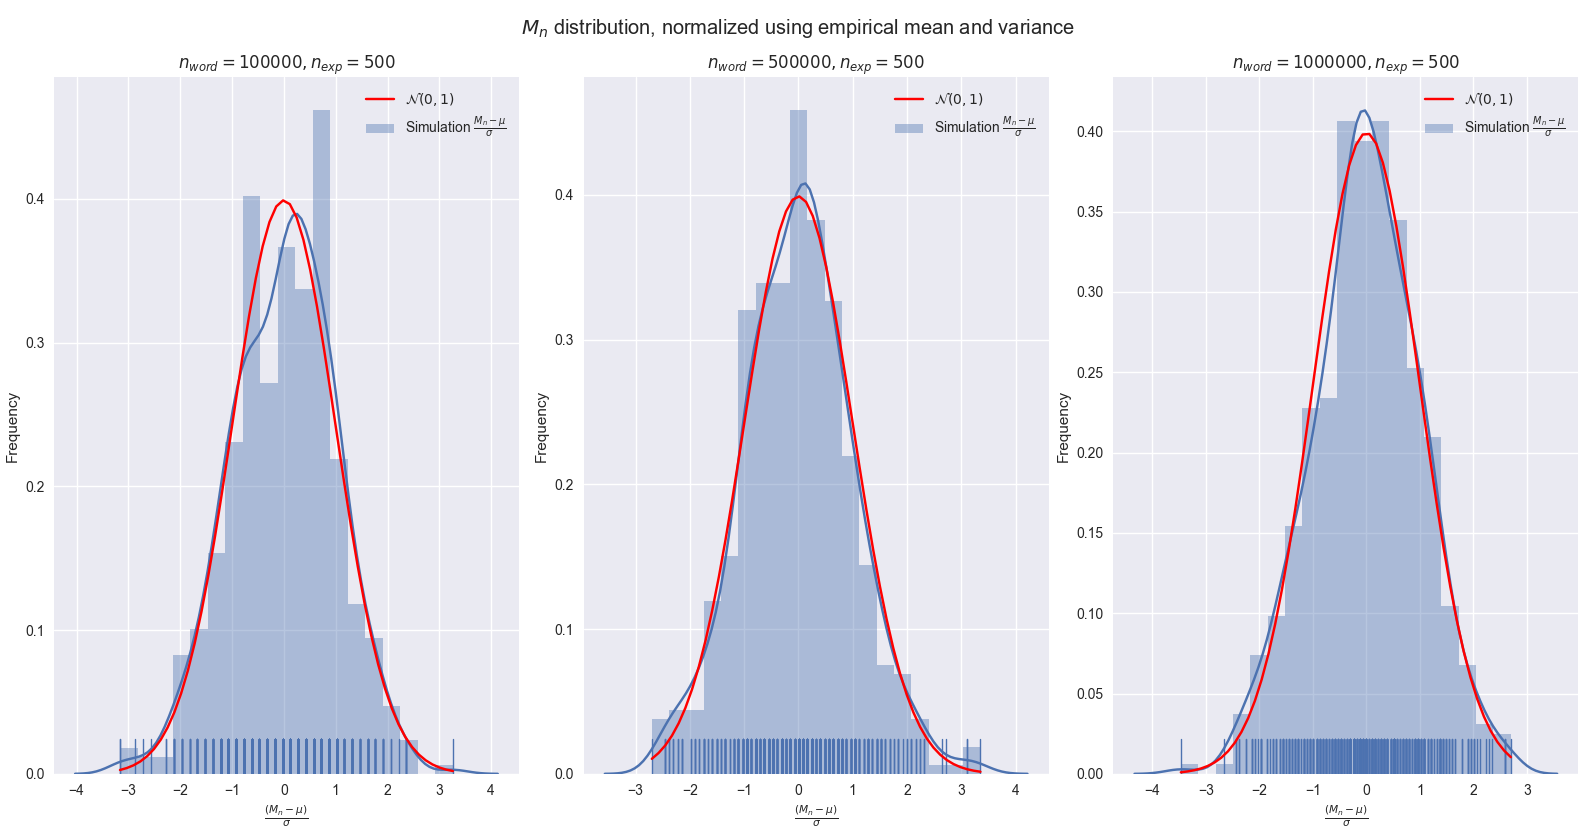
\includegraphics[width = \textwidth]{empirical_normalization_10e6_500.png}
\end{frame}

\begin{frame}{Hypothesis testing for the variance}

		\begin{block}{ Complex matrix }
			Defining $P(s)$ as 
			$
			\begin{array}{rl}
				p_{1 1}^{-s} & p_{1 2}^{-s} \\
				p_{2 1}^{-s} & p_{2 2}^{-s} 
			\end{array}
			$
		\end{block}

		\begin{block}{ Variance expression }
			\centers{$ V_n =  \left( \ddot{\lambda}(-1) - { \dot{\lambda}(-1) }^2 \right) \f{n}{\ln^2 n} $}
		\end{block}
\end{frame}

\begin{frame}
	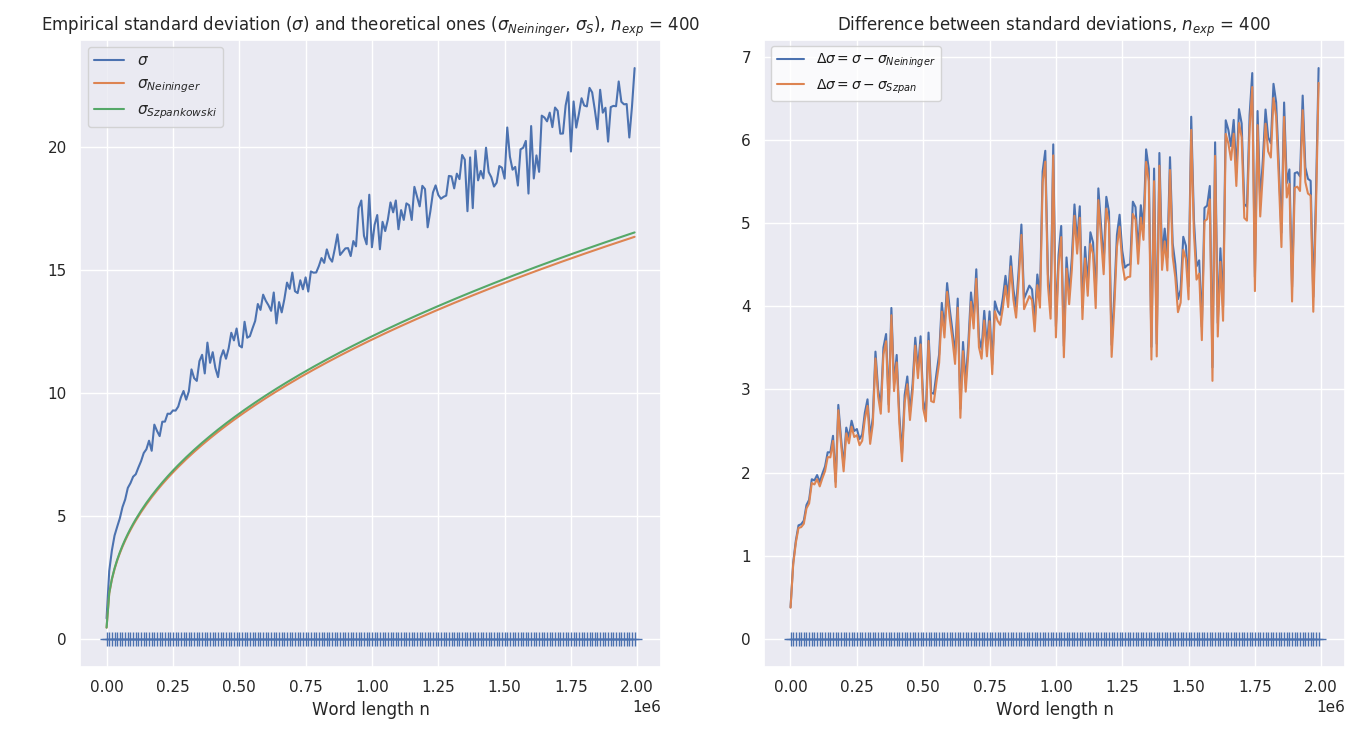
\includegraphics[width = \textwidth]{eig_fig1.png}
\end{frame}


\section{ Analytic information theory }

\subsection{ Power series }
	\begin{frame}{ Definition, usage }
		\begin{block}{Definition}
			\centers{$ A(z) = \Sum{n\geq0}a_n z^n$}
		\end{block}

		\begin{block}{Remarks}
			\begin{itemize}
				\item Used as an algebraic item with the convolution product
				\item No convergence problems
			\end{itemize}
		\end{block}

	\end{frame}

\subsection{ Complex analysis tools }

	\begin{frame}

	\begin{block}{Poissonization and Depoissonization}
		\centers{${\tilde G}(z) = \Sum{n\geq 0}{} a_n \f{z^n}{n!} \ex{-z} $}
	\end{block}

	\begin{block}{Mellin transform}
		Make recurrence relation between random variables
		become linear in order to solve them more easily.
	\end{block}

	\end{frame}

\section{ Application to covariance analysis }

	\subsection{ Tail symbols }

		\begin{frame}{Tail symbols}

			\begin{block}{ Illustration }
				\begin{egalites}
	& X(1) 
		& {\color{red}{0}} {\color{green}{0}} 00000\dots \\
	&X(2) 
		& {\color{red}{1}} {\color{green}{0}}10101\dots \\
	& X(3) 
		& {\color{red}{10}} {\color{green}{0}} 1101 \dots \\
	& X(4) 
		& {\color{red}{00}} {\color{green}{1}} 100111\dots
	\end{egalites}
			\end{block}

			\begin{block}{Definition}
				Let $c$ be a character from our alphabet $\{ a, b \}$.
				In the case when all the sequences start with a $c$, we 
				define $T_n^{\,c}$ the \emph{number of times $a$ is a tail symbol in 
				the experiment}.
			\end{block}

		\end{frame}

		\begin{frame}{Definition and relation}

			

			\begin{block}{Recurrence}
				For $n \geq 0$, we have :
					\[ \boxed{ T_{n+1}^{\,c} = \delta_a + 
											{{\tilde T}_{N_a}}^a
											+ {{\tilde T}_{N_b}}^b } \]
			\end{block}
		
			\begin{block}{ Notations }
				\begin{itemize}
				\item $\delta_a = 
							\begin{cases} 
								1 & \text{if $a$ is the tail symbol of the
										first sequence}\\
								0 & \text{else} 
							\end{cases}$

				\item $N_a$ is the 
				random variable giving \emph{the size of the left subtree 
				which contains phrases whose second letter is $a$}

				\item ${{\tilde T}_{N_a}}^a$ is the number of 
				times $a$ is a tail symbol for the sequences that were 
				used to  build the subtree with phrases having $a$ as second
				symbol.

				\item $T_0^c$ for all $c$ by convention.
			\end{itemize}
			\end{block}

		\end{frame}

		\begin{frame}{Total path lenght}

			\begin{block}{Definition}
				Defining $L_n^{\,c}$ as the \emph{total 
				path length of the nodes of the DST that was built with
				MI model with $n$ sequences starting with letter $c$}.
				It is the sum of the lengths of all the prefix phrases.
			\end{block}

			\begin{block}{Recurrence relation}
				For all $n\geq 0$ :

				\[
				\boxed{ 
					L_{n+1}^c = n + 
										{{\tilde L}_{N_a}}^a + 
										{{\tilde L}_{N_b}}^b
				}
				\]
			\end{block}
		\end{frame}

	\subsection{Simulation results}

		\begin{frame}
			Inconclusive, but informative
		\end{frame}

	\subsection{Analytic solution}

		\begin{frame}
			\begin{block}{Recurrence}
			  \[ \boxed{ \Cov(T_{n+1}^{\,c}, L_{n+1}^c) = 
          \Cov ( {{\tilde T}_{N_a}}^a,
                         {{\tilde L}_{N_a}}^a )
          + \Cov ( {{\tilde T}_{N_b}}^b, 
                          {{\tilde L}_{N_b}}^b ) } \]
			\end{block}
		\end{frame}

		\begin{frame}
			\begin{block}{Poisson transform}
				Defining 
  \[ \boxed{ C_c(z) 
            = \Sum{n\geq0}{} \Cov(T_n^{\,c}, L_n^{\,c}) 
                            \f{z^n}{n!} \ex{-z} } \]
			\end{block}

			\begin{block}{Differential equation}
							\[
			\boxed{
			\partial_z C_c(z) + C_c(z) 
				= C_a(zp) + C_b(zq)
			}
			\]
			\end{block}
		\end{frame}

\begin{frame}
	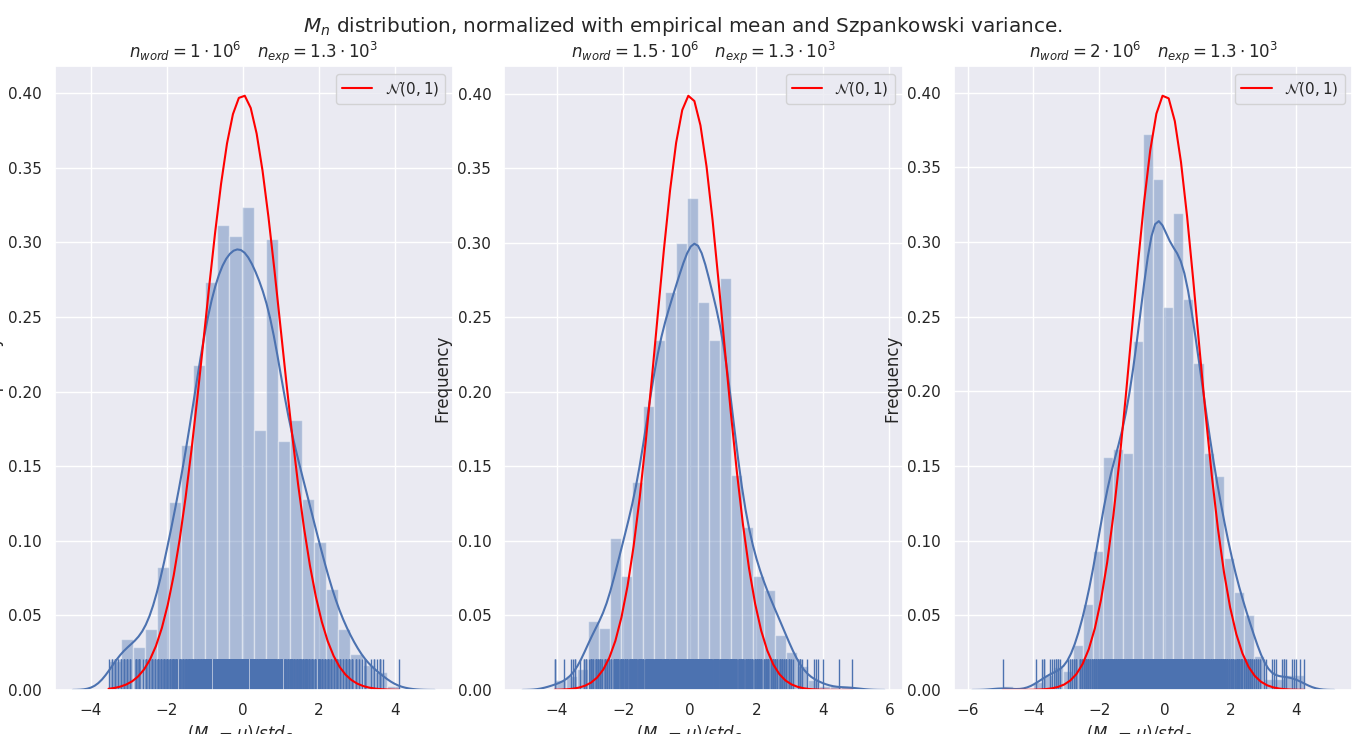
\includegraphics[width=\textwidth]{eig_fig2.png}
\end{frame}


\begin{frame}
	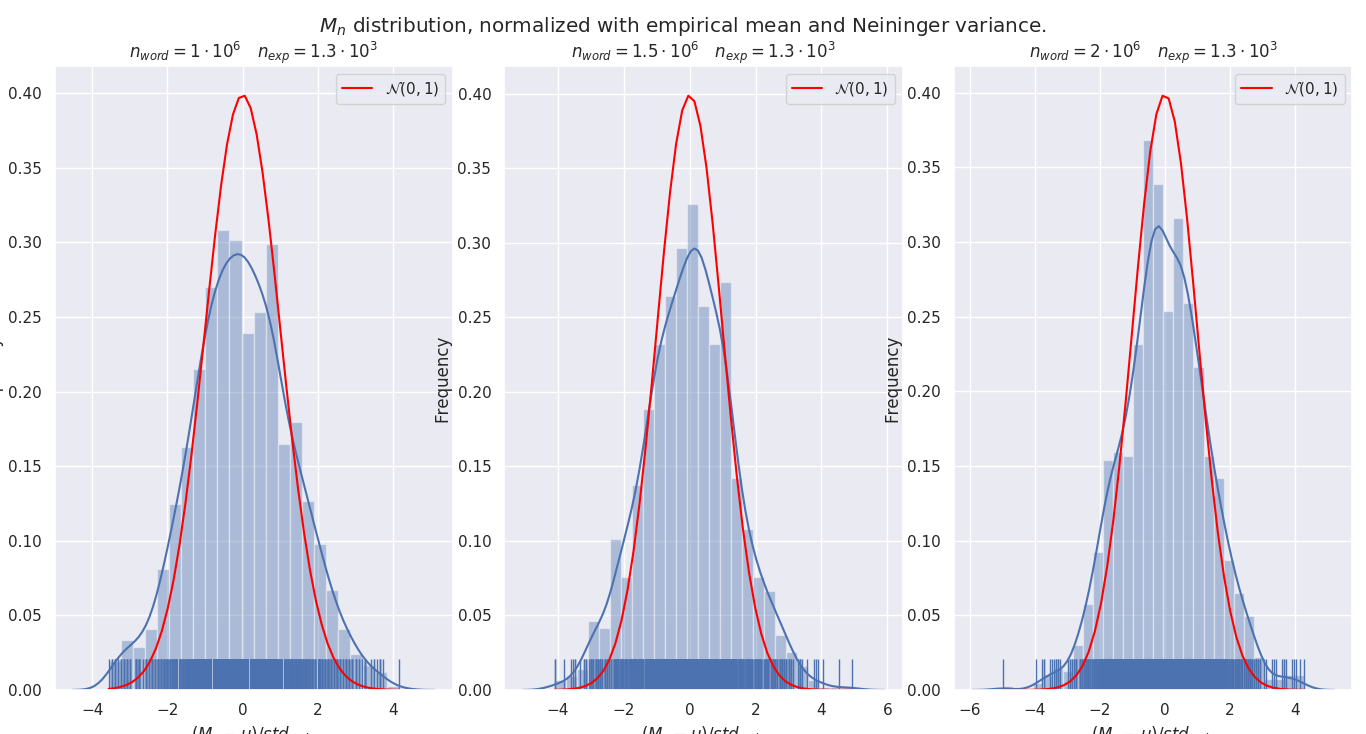
\includegraphics[width=\textwidth]{eig_fig3.png}
\end{frame}


\begin{frame}
	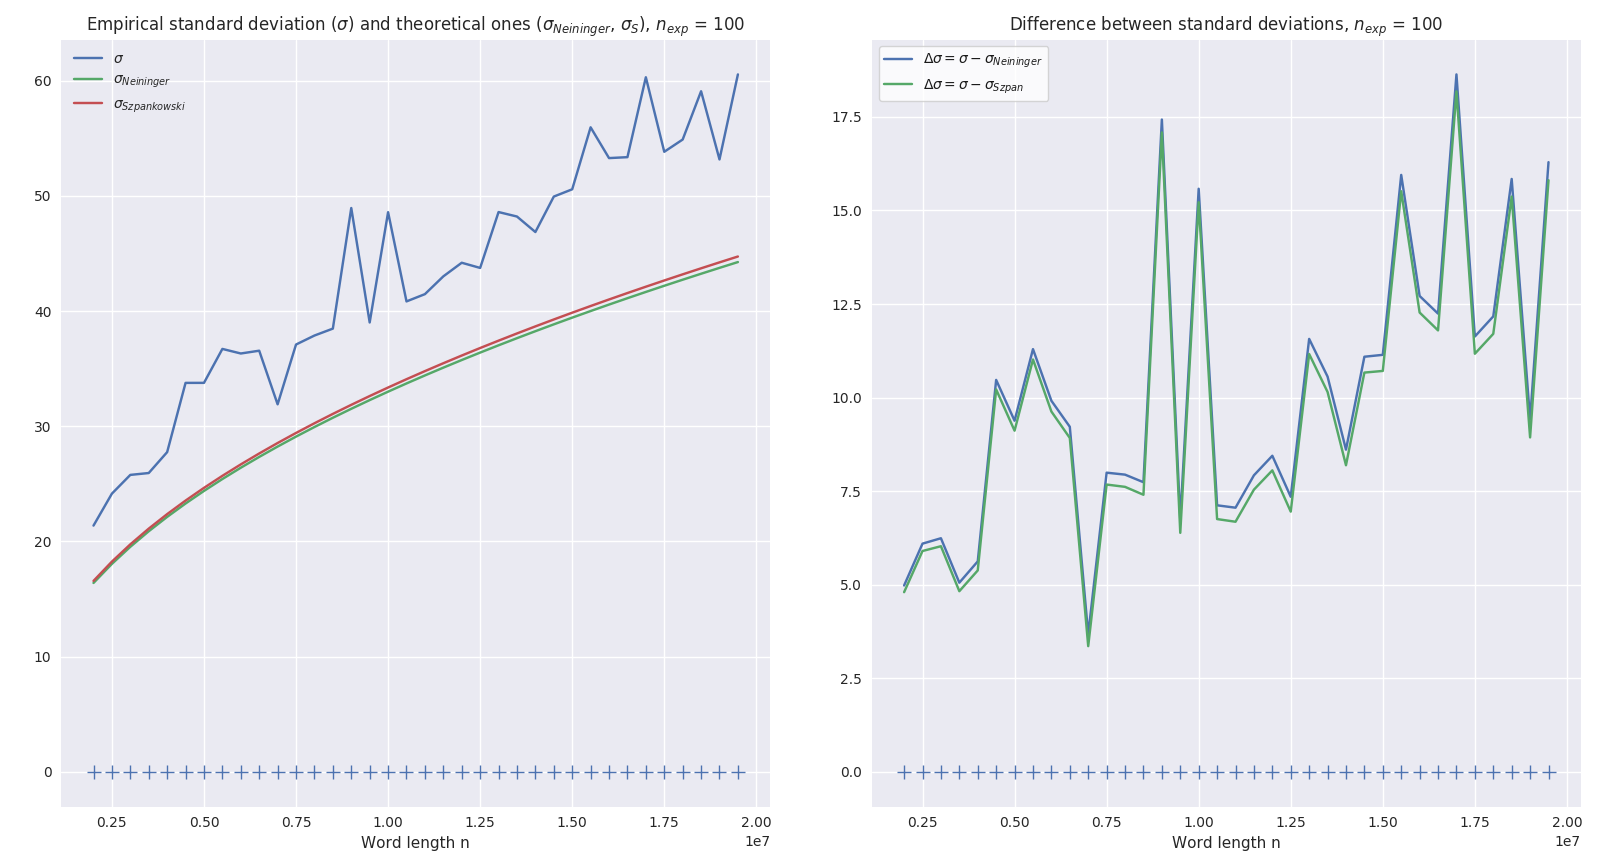
\includegraphics[width=\textwidth]{eig_fig4.png}
\end{frame}


\begin{frame}
	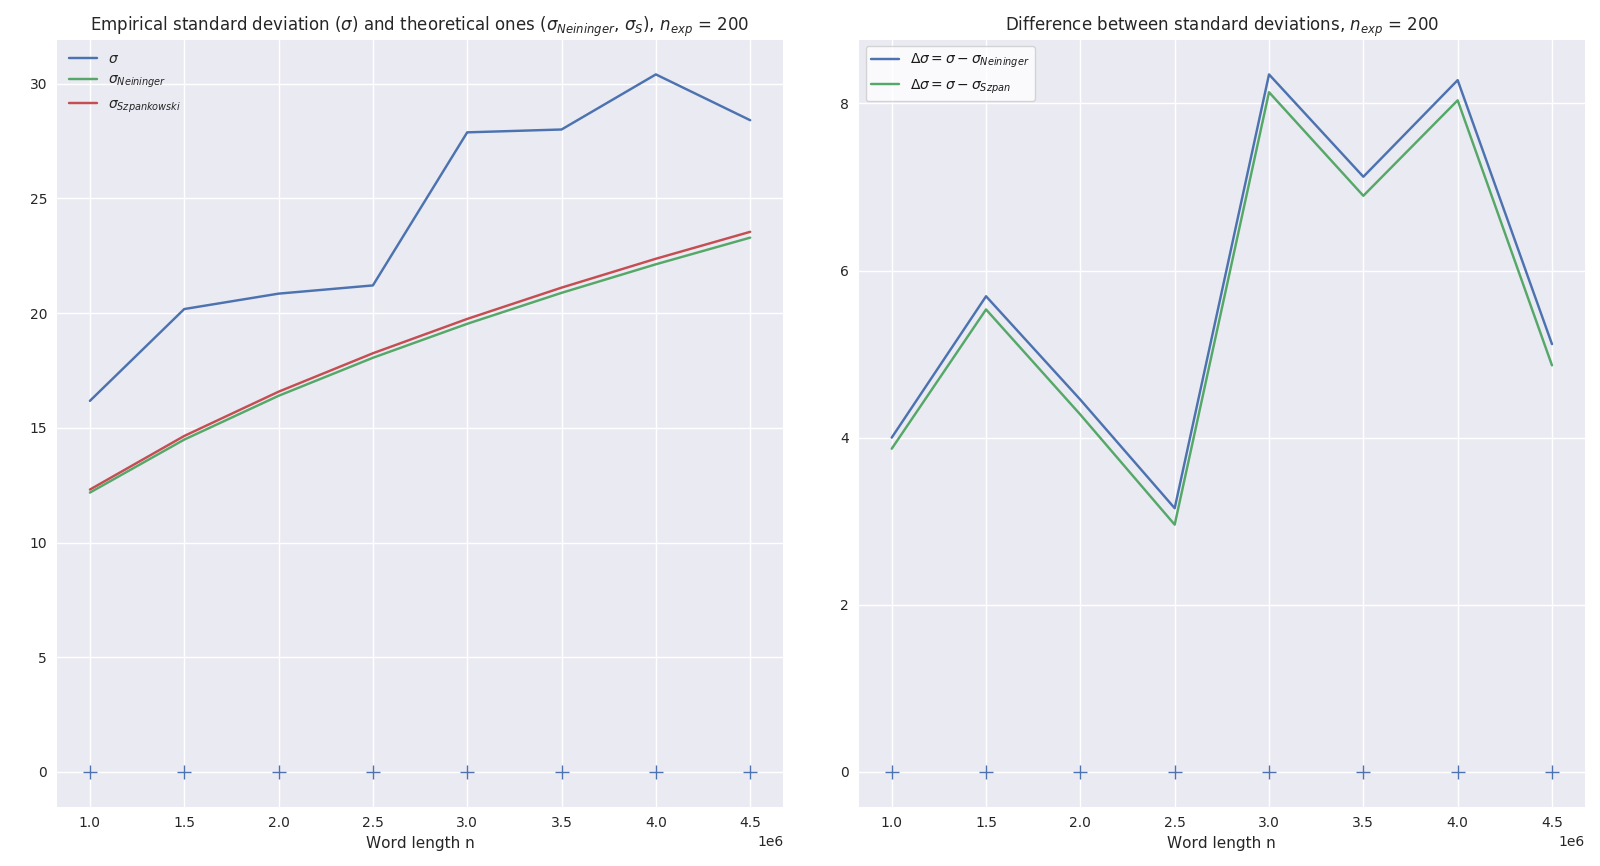
\includegraphics[width=\textwidth]{eig_fig5.png}
\end{frame}

\begin{frame}[allowframebreaks]
\nocite{*}
\bibliographystyle{unsrt}
\bibliography{sample}
\end{frame}

\end{document}
